%%%%%%%%%%%%%%%%%%%%%%%%%%%%%%%%%%%%%%%%%%%%%%%%%%%%%%%%%%%%%%%%%%%%%%%
%                                                                     %
%                      UNIVERSIDAD de la Repblica                     %
%               Facultad de Ingeniera			             		  %
%                                                                     %
%                              ------------------                     %
%                             | FORMATO DE TESIS |                    %
%                              ------------------                     %
%                                                                     %
%                           (C) Samuel Oporto Daz                     %
%                         (C) Brucele Tejeda Medrano                  %
%                                                                     %
%                                     2006                            %
%                                                                     %
%%%%%%%%%%%%%%%%%%%%%%%%%%%%%%%%%%%%%%%%%%%%%%%%%%%%%%%%%%%%%%%%%%%%%%%


\documentclass[12pt,oneside,final]{rf2}
\hyphenation{Ber-ge-ret} %se indican las sílabas para que lo "recorte" bien cuando termina un renglón
\hyphenation{si-guien-te} 
 \usepackage{hyperref}
 \hypersetup{colorlinks=true,    % false: boxed links; true: colored links
    linkcolor=black,          	 % color of internal links
    citecolor=blue,        		 % color of links to bibliography
    filecolor=black,      		 % color of file links
    urlcolor=blue          		 % color of external links
}

\usepackage{array}
\usepackage{longtable} 
\usepackage{multicol} 
\usepackage{epsfig,bm,epsf,float}

%\usepackage[usenames,dvipsnames]{color}

\usepackage[utf8]{inputenc} %si esta no funciona descomentar la de abajo
%\usepackage[latin1]{inputenc} %si esta no funciona descomentar la de arriba
\usepackage[activeacute,spanish]{babel}

\usepackage{graphicx}

\usepackage[usenames]{color}
\usepackage{times}
\usepackage{subfigure}
\usepackage{longtable}
\setlength{\arrayrulewidth}{1pt}
\setlength{\doublerulesep}{0mm}
\usepackage{multirow}
\usepackage{pdfpages}


%\usepackege{tabulary}

\begin{document}

% Portada:

% Nombre de tesis
\title{$RF^{2}$}

% Autor
\author{Daniel Aicardi, Melina Rabinovich, Edgardo Vaz}

% Mes
\degreemonth{Julio}

% Año
\degreeyear{2011}

% Título profesional
\degree{}

% Asesor
\advisor{Ing. Juan Pablo Oliver, Ing. Andr\'es Aguirre}

\maketitle











\begin{abstract}
\begin{itshape}
\dsp

El presente documento describe el prototipo Recarga Fácil por Radio Frecuencia, RF$^{2}$, realizado como proyecto de fin de carrera de Ingeniería Eléctrica en la Universidad de la República entre marzo de 2010 y julio de 2011. El mismo consiste en un sistema embebido para recarga y consulta de tarjetas RFID, como las que se utilizan hoy día en el sistema de transporte metropolitano, y fue diseñado para operar de forma autónoma interactuando directamente con el usuario.

\bigskip
El hardware fue enteramente diseñado por el grupo de trabajo a excepción de la single board computer. Las herramientas de software utilizadas son open source, así como también las bibliotecas usadas para desarrollar la aplicación final. El diseño, la fabricación, y el armado del prototipo fue realizado en su totalidad en Uruguay.

\end{itshape}
\end{abstract}

\begin{acknowledgments}

En primer lugar queremos agradecer a nuestras familias y amigos. Agradecemos a Leonardo Steinfeld, Nicolás Barabino, Francisco Lanzari, María Eugenia Corti, Santiago Reyes, Viterbo Rodríguez, Christian Gutierrez, Andrés Bergeret, Gonzalo Tabares, Klaus Rotzinger, Marcelo Fiori, Pablo Cancela, Ana y Claudia Rabino. Y a todos los que de alguna u otra forma colaboraron con nosotros.

\end{acknowledgments}
% -----------------------------------------------------------------------------------------------------------------
% Cambiar dedicatoria...
% -----------------------------------------------------------------------------------------------------------------


\dedication

\begin{quote}

para cuchu,\\
chuchuchu,\\
y pirimpirim jajaja

\end{quote}
\begin{prefacio}

\begin{itshape}
“El ciudadano Línea saca su billetera, extrae su tarjeta y la introduce en la máquina registradora; una serie de gestos automáticos. Unas mandíbulas de aluminio se cierran sobre ella, unos dientes de cobre buscan la clave magnética, y una lengua electrónica saborea la vida del ciudadano Línea.
Lugar y fecha de nacimiento. Padres. Raza. Religión. Historial educativo, militar y de servicios civiles. Estado. Hijos. Ocupaciones, desde el comienzo hasta el presente. Asociaciones. Medidas físicas, huellas digitales, retínales, grupo sanguíneo. Grupo psíquico básico. Porcentaje de lealtad, índice de lealtad en función del tiempo hasta el momento del último análisis...
... El ciudadano Línea se encuentra en la ciudad donde, la noche anterior, dijo que estaría, así que no ha tenido que hacer una corrección.
Los nuevos informes se añaden al historial del ciudadano Línea. Toda su vida regresa al banco de datos. Desaparece de la unidad exploradora y la unidad comparativa, para que éstas atiendan la próxima llegada.
La máquina ha tragado y digerido otro día. Está satisfecha.”

\rightline{Sam Hall (1953), Poul Anderson}
\end{itshape}
\bigskip

La narración anterior es parte de un cuento de ciencia ficción llamado “Sam Hall”, escrita por Poul Anderson en 1953. En esta historia el autor describe un mundo donde cada persona tiene asignada una tarjeta conteniendo datos que la caracterizan, y puede ser controlado su accionar a través de una super computadora que almacena y procesa los datos de toda la humanidad. 
En nuestros días este cuento de ciencia ficción no está tan alejado de la realidad, las tarjetas “inteligentes” (smart cards) son cada vez más usadas en múltiples aplicaciones como ser, pasaporte electrónico, pago electrónico, sistemas de transporte, controles de acceso y sistemas de seguridad, entre otros.
El siguiente proyecto se desarrolla con la intención de aprender las bases del mundo de las tarjetas “inteligentes” y que sirva como punto de partida para que otros entiendan su funcionamiento. 
No es intención de los autores que se use el contenido de este documento con fines como los que se indicaban en la narrativa de ciencia ficción, muy por el contrario, el empleo de esta tecnología debe estar en favor de las personas y no en su contra.

\end{prefacio}
\newpage
\addcontentsline{toc}{section}{Tabla de contenidos}

\tableofcontents

\listoffigures

\listoftables
\newpage
\startarabicpagination

% Capítulos ---> esto define el índice
\part{Introducci\'on}
\chapter{Descripci\'on del proyecto}

\section{Definici\'on}

A partir de la puesta en marcha del sistema de transporte metropolitano, surge la necesidad de consultar y recargar tarjetas RFID (utilizadas en dicho sistema) en l\'inea con un servidor, de forma r\'apida, segura y autogestionada por parte del usuario, en diversos puntos de Montevideo.

\section{Antecedentes}

\begin{itemize}

\item AFE: Prototipo de sistema embebido capaz de cargar y consultar tarjetas RFID como las utilizadas en el sistema de transporte metropolitano. El mismo se compone de varios m\'odulos: una SBC (single board computer), un lector-escritor de tarjetas RFID, un lector de tarjetas de contacto, un m\'odem 3G/GPRS y una interfaz con el usuario que consta de un display, leds y buzzer.

\item OpenPCD: Dise'no de hardware libre para dispositivos de proximidad de acoplamiento (PCD) basado en comunicaci\'on RF de 13,56MHz. Este dispositivo es capaz de desplegar informaci\'on desde Tarjetas de proximidad de Circuito Integrado (PICC) que se ajusten a las normas de proveedores independientes, tales como ISO 14443, ISO 15693, as\'i como los protocolos propietarios como Mifare Classic.

\end{itemize}
\chapter{Objetivo general del proyecto}

\section{?`Qu\'e y para qu\'e?}

En principio, el objetivo del proyecto era realizar un prototipo de sistema embebido mediante el cual se pudiera interactuar con tarjetas RFID (basadas en las normas ISO 14443) como las usadas en el STM.
Mejorar la arquitectura actual del dispositivo AFE rompiendo dependencias tecnol\'ogicas con el actual lector-escritor de tarjetas Mifare.

Para lograrlo se partir\'ia de la base de un dispositivo open-hardware y open-firmware (OpenPCD).
Generar conocimiento dentro de la Divisi\'on Tecnolog\'ia de la Informaci\'on de la Intendencia de Montevideo.

Luego se dej\'o de lado el partir del dispositivo OpenPCD, para lograr un dise'no propio de lector-escritor de tarjetas RFID.

\section{?`Por qu\'e cambiar la arquitectura actual?}

Como arquitectura precedente existe la del prototipo AFE (Artefacto Feo de Exhibir), realizada por el grupo de electr\'onica de la IM. La misma consiste en una SBC, que se fabrica con otro prop\'osito y es utilizada en esta aplicaci\'on puesto que es la \'unica forma de adquirir este tipo de hardware en plaza. A \'esta se conectan a trav\'es de puertos USB, un lector-escritor de tarjetas Mifare, un lector de tarjetas de contacto, un modem 3G y un dispositivo dise'nado a partir de un microcontrolador PIC, llamado USB4ALL, el cual es open-hardware y open-firmware, en el que se pueden conectar otro tipo de dispositivos cuya interfaz nativa no sea USB, como ser displays, buzzer, leds, sensores, etc, los cuales no pueden ser conectados directamente a la SBC porque la misma no cuenta con los puertos de expansi\'on necesarios.

Surge entonces la necesidad de cambiar la configuraci\'on de dicha arquitectura. Se hace necesario romper dependencias tecnol\'ogicas con el lector-escritor de tarjetas Mifare, ya que dej\'o de ser soportado por la librer\'ia pcsclite (a pedido del fabricante); y con la SBC, que es empleada en una aplicaci\'on espec\'ifica y puede dejar de fabricarse o sufrir cambios dr\'asticos que ya no permitan su uso.


\section{Alcance}

\begin{itemize}

\item Hardware: Se fabricar\'a un m\'odulo donde se insertar\'a la tarjeta de contacto (SAM).
      Se agregar\'a un display LCD 16x2, leds y buzzer como interfaz para el usuario. Se fabricar\'a un m\'odulo de lectura-escritura RFID. Se estudiar\'a la forma de conectar los perif\'ericos a la placa de la SBC.

\item Software: Se har\'a lo necesario para que el lector-escritor RFID funcione como un dispositivo soportado por la librer\'ia pcsclite empleada en sistemas operativos Linux para interactuar con lectores de tarjetas. Con esto se lograr\'a compatibilidad hacia atr\'as, de modo de poder reutilizar las aplicaciones desarrolladas para el dispositivo AFE.
    
\end{itemize}

\section{Especificaci\'on funcional}

El prototipo final deber\'a ser capaz de interactuar con tarjetas RFID a trav\'es de la antena del dispositivo lector-escritor RFID, y con una tarjeta de contacto. Luego de los controles correspondientes y autenticaci\'on de la tarjeta (con datos encriptados), comenzar\'a la interacci\'on con el usuario mediante un display LCD16x2 que ser\'a la interfaz de comunicaci\'on con el mismo. El display informar\'a al usuario de las tareas que se est\'en realizando, mensajes cortos y descriptivos. Los tiempos de recarga y consulta deber\'an ser menores a un minuto.

\section{Criterios de \'exito}

\begin{itemize}

\item Lograr recargar y consultar tarjetas RFID mediante el dispositivo embebido, el cual estar\'a en comunicaci\'on directa con la infraestructura STM.

\item Los tiempos de recarga y consulta deber\'an ser menores a un minuto.

\end{itemize}
\part{Dise'no}
\chapter{Funcionamiento del prototipo}

\section{Requerimientos}
El principal requerimiento a cumplir es la interacción con tarjetas RFID (ver apéndice \ref{anx_sc}), tanto para su lectura como escritura.
La comunicación con tarjetas de contacto (ver apéndice \ref{anx_sc}) es necesaria para la interacción con un módulo de seguridad que permita, la generación de las claves utilizadas para autenticarse con las tarjetas RFID, y una transacción segura con un servidor. En ambos casos es necesario cumplir con las normas y estándares adecuados  (tarjetas RFID - ISO 14443 y tarjetas de contacto - ISO7816).
Por último mantener informado al usuario de lo que sucede durante una transacción a través de una interfaz visual y sonora.


\section{Descripción del prototipo}
Este prototipo integra la lista de dispositivos que hoy en día se denominan sistemas embebidos. Su hardware está integrado por un sistema basado en un microprocesador que  recibe el nombre de Single Board Computer (SBC), a la que se agrega un conversor de niveles (VLT) que permite interconectarla con, un lector/escritor de tarjetas RFID a través de un puerto SPI, un lector de tarjetas de contacto a través de un puerto serial (UART), y la interfaz de usuario compuesta por un buzzer, tres leds (rojo, amarillo, verde) y un display conectado a través de puertos de entrada/salida de propósito general (GPIO).

\begin{figure}[H]
\centering
  \begin{center}
   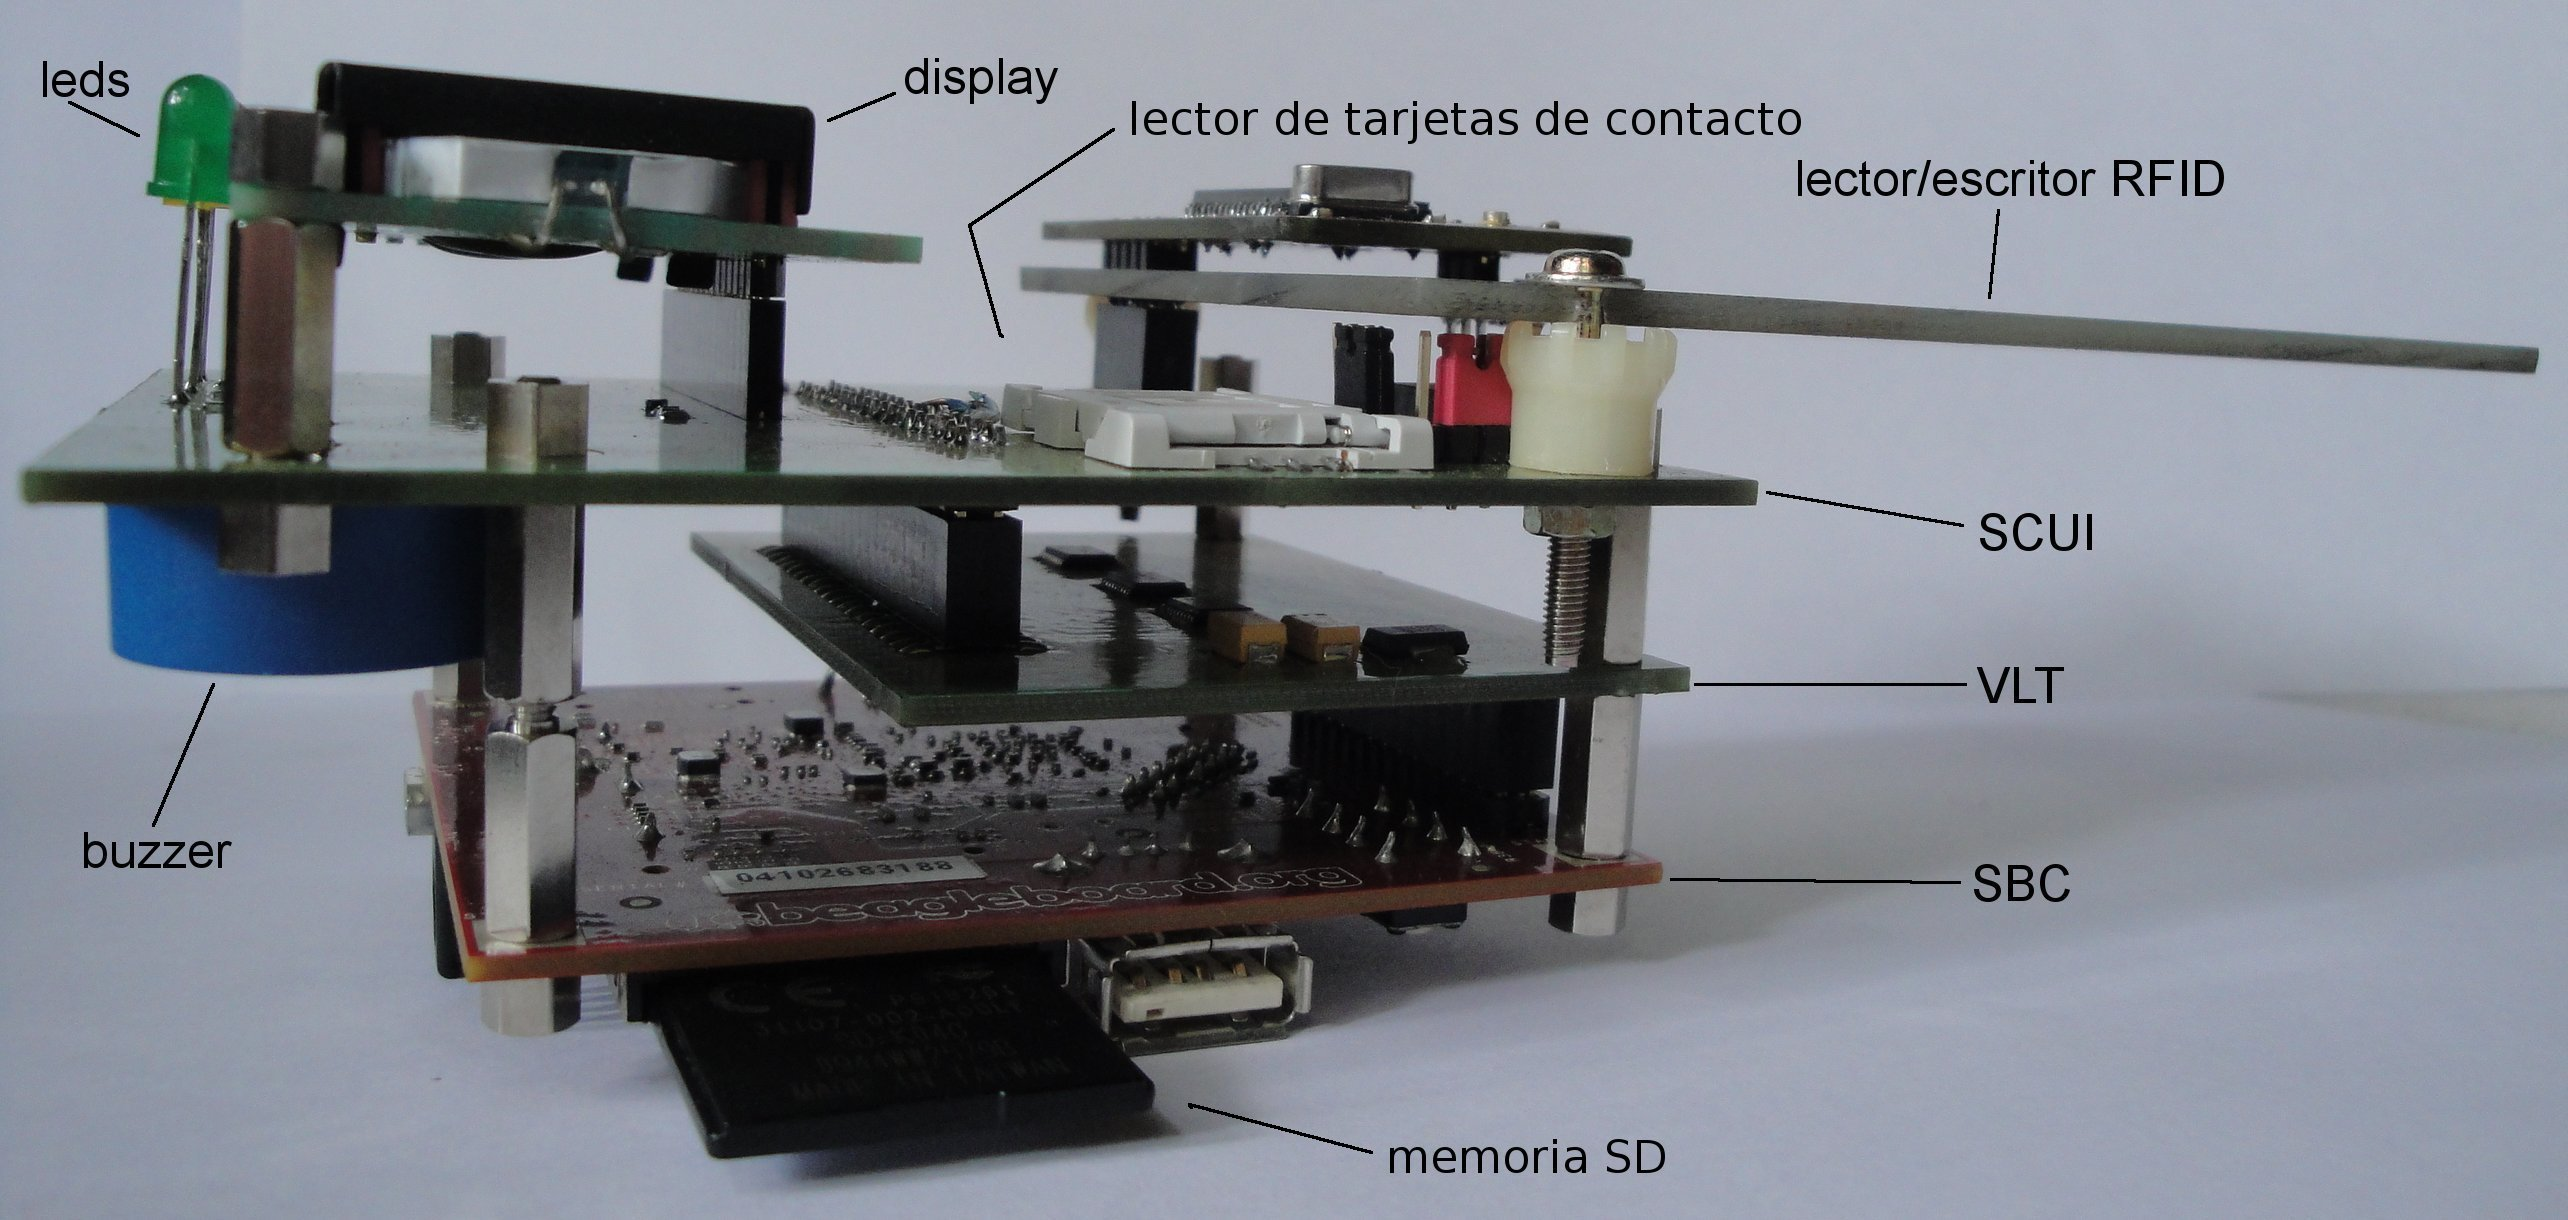
\includegraphics[scale=.15]{Imagenes/prototipo_s_nombres.jpg}
  \end{center}
  \caption{Vista general del prototipo}\label{prototipo} 
\end{figure}

\begin{figure}[H]
  \centering
  \subfigure[Vista anversa del prototipo]{\label{protoF}
  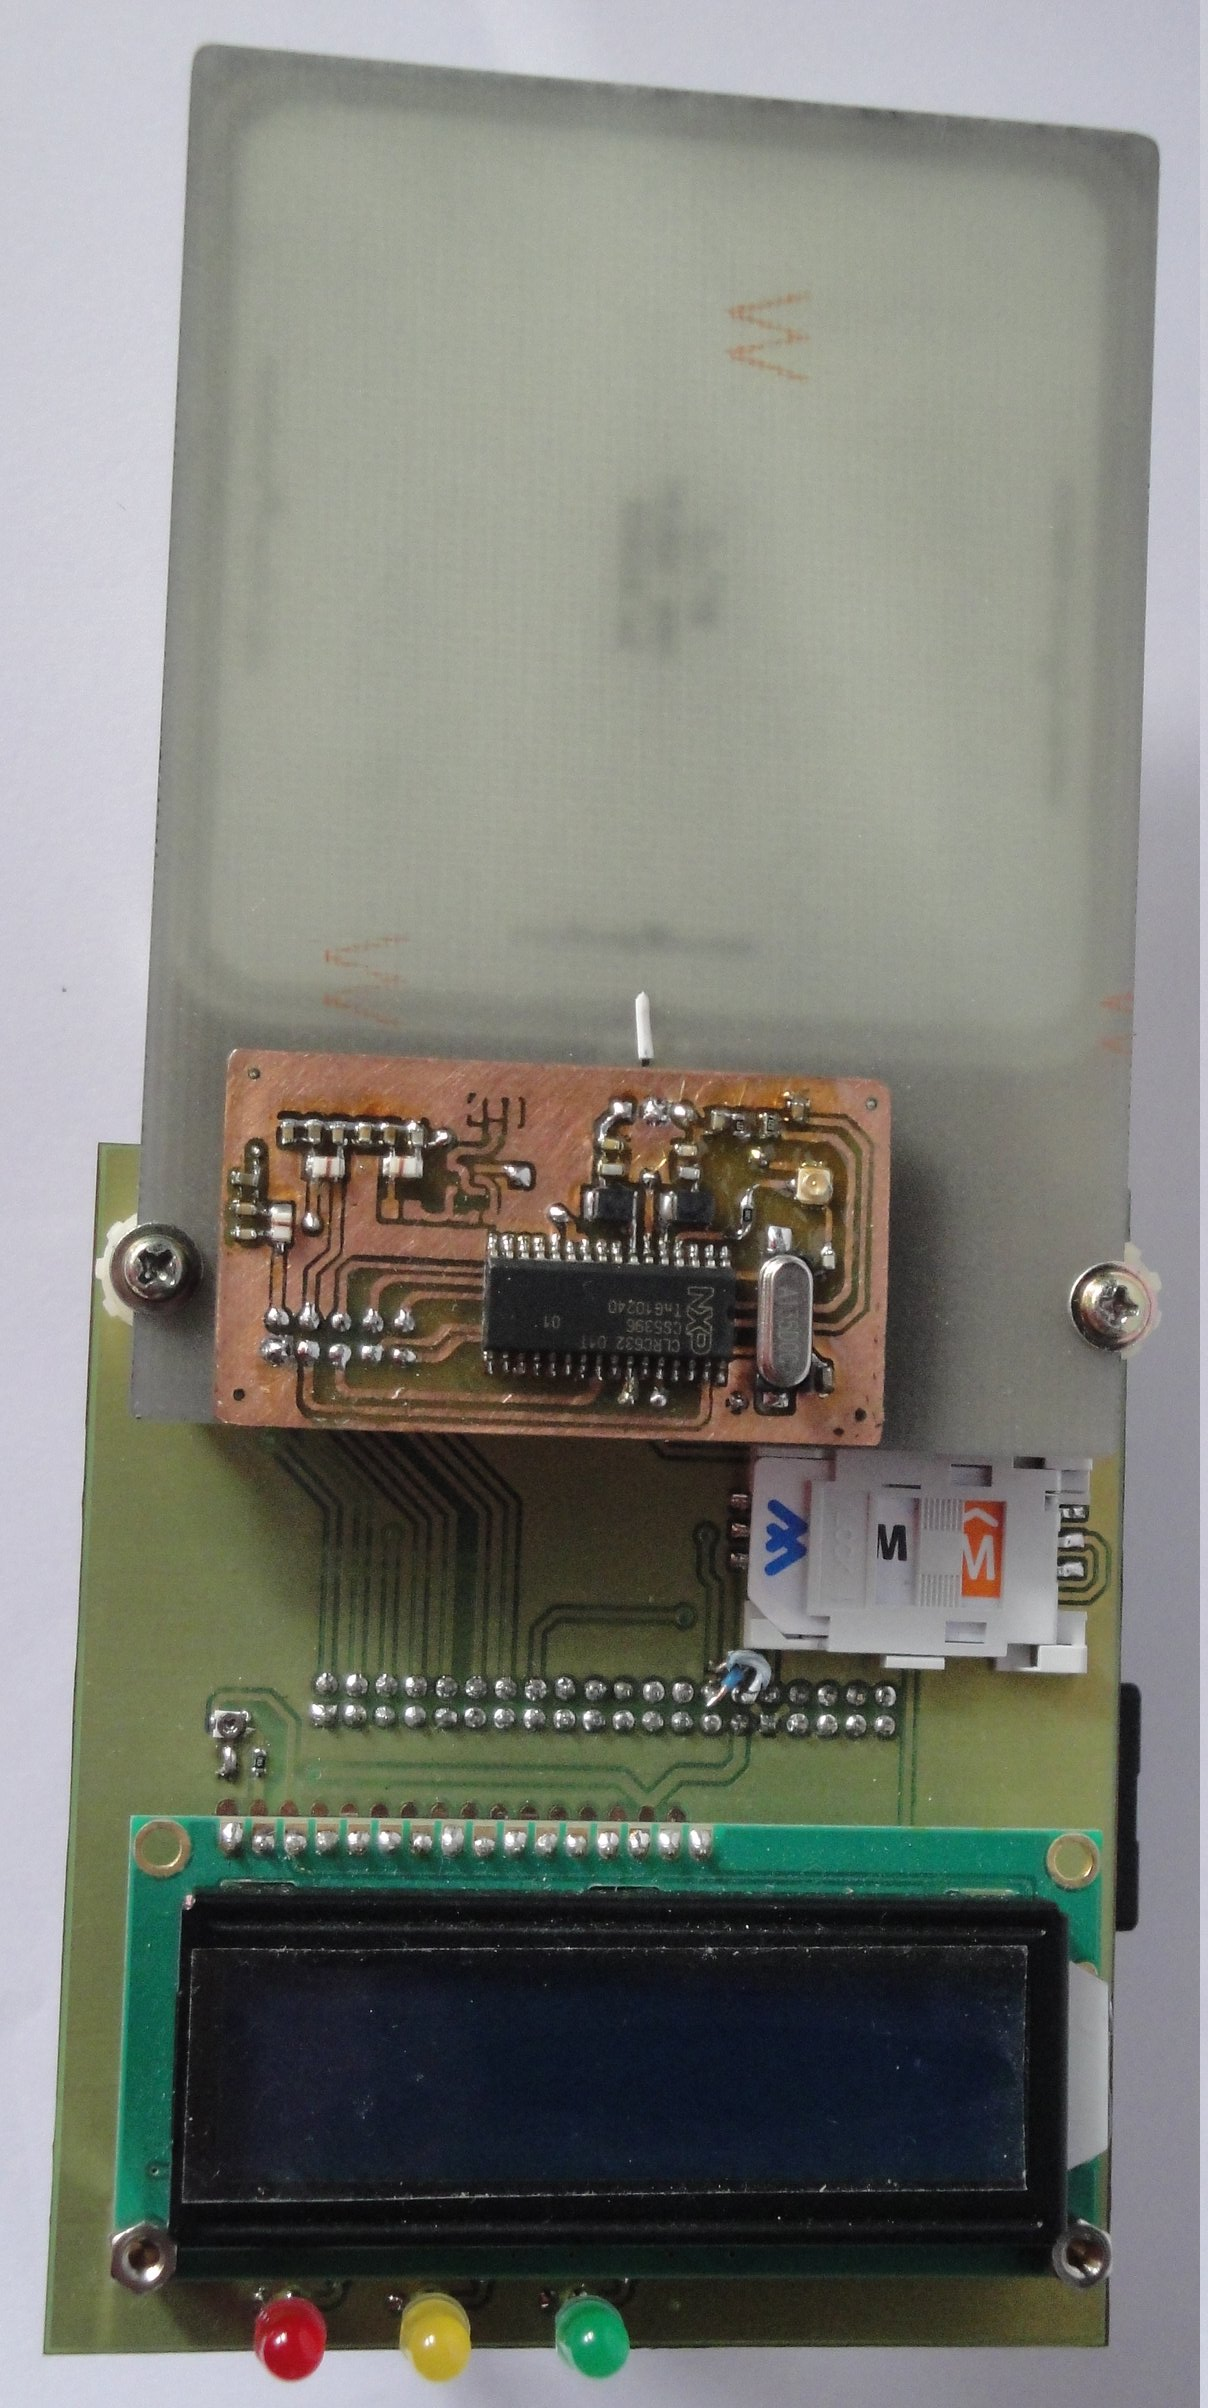
\includegraphics[scale=.13]{Imagenes/prototipo_f.jpg} } 
  \subfigure[Vista reversa del prototipo]{\label{protoB} 
  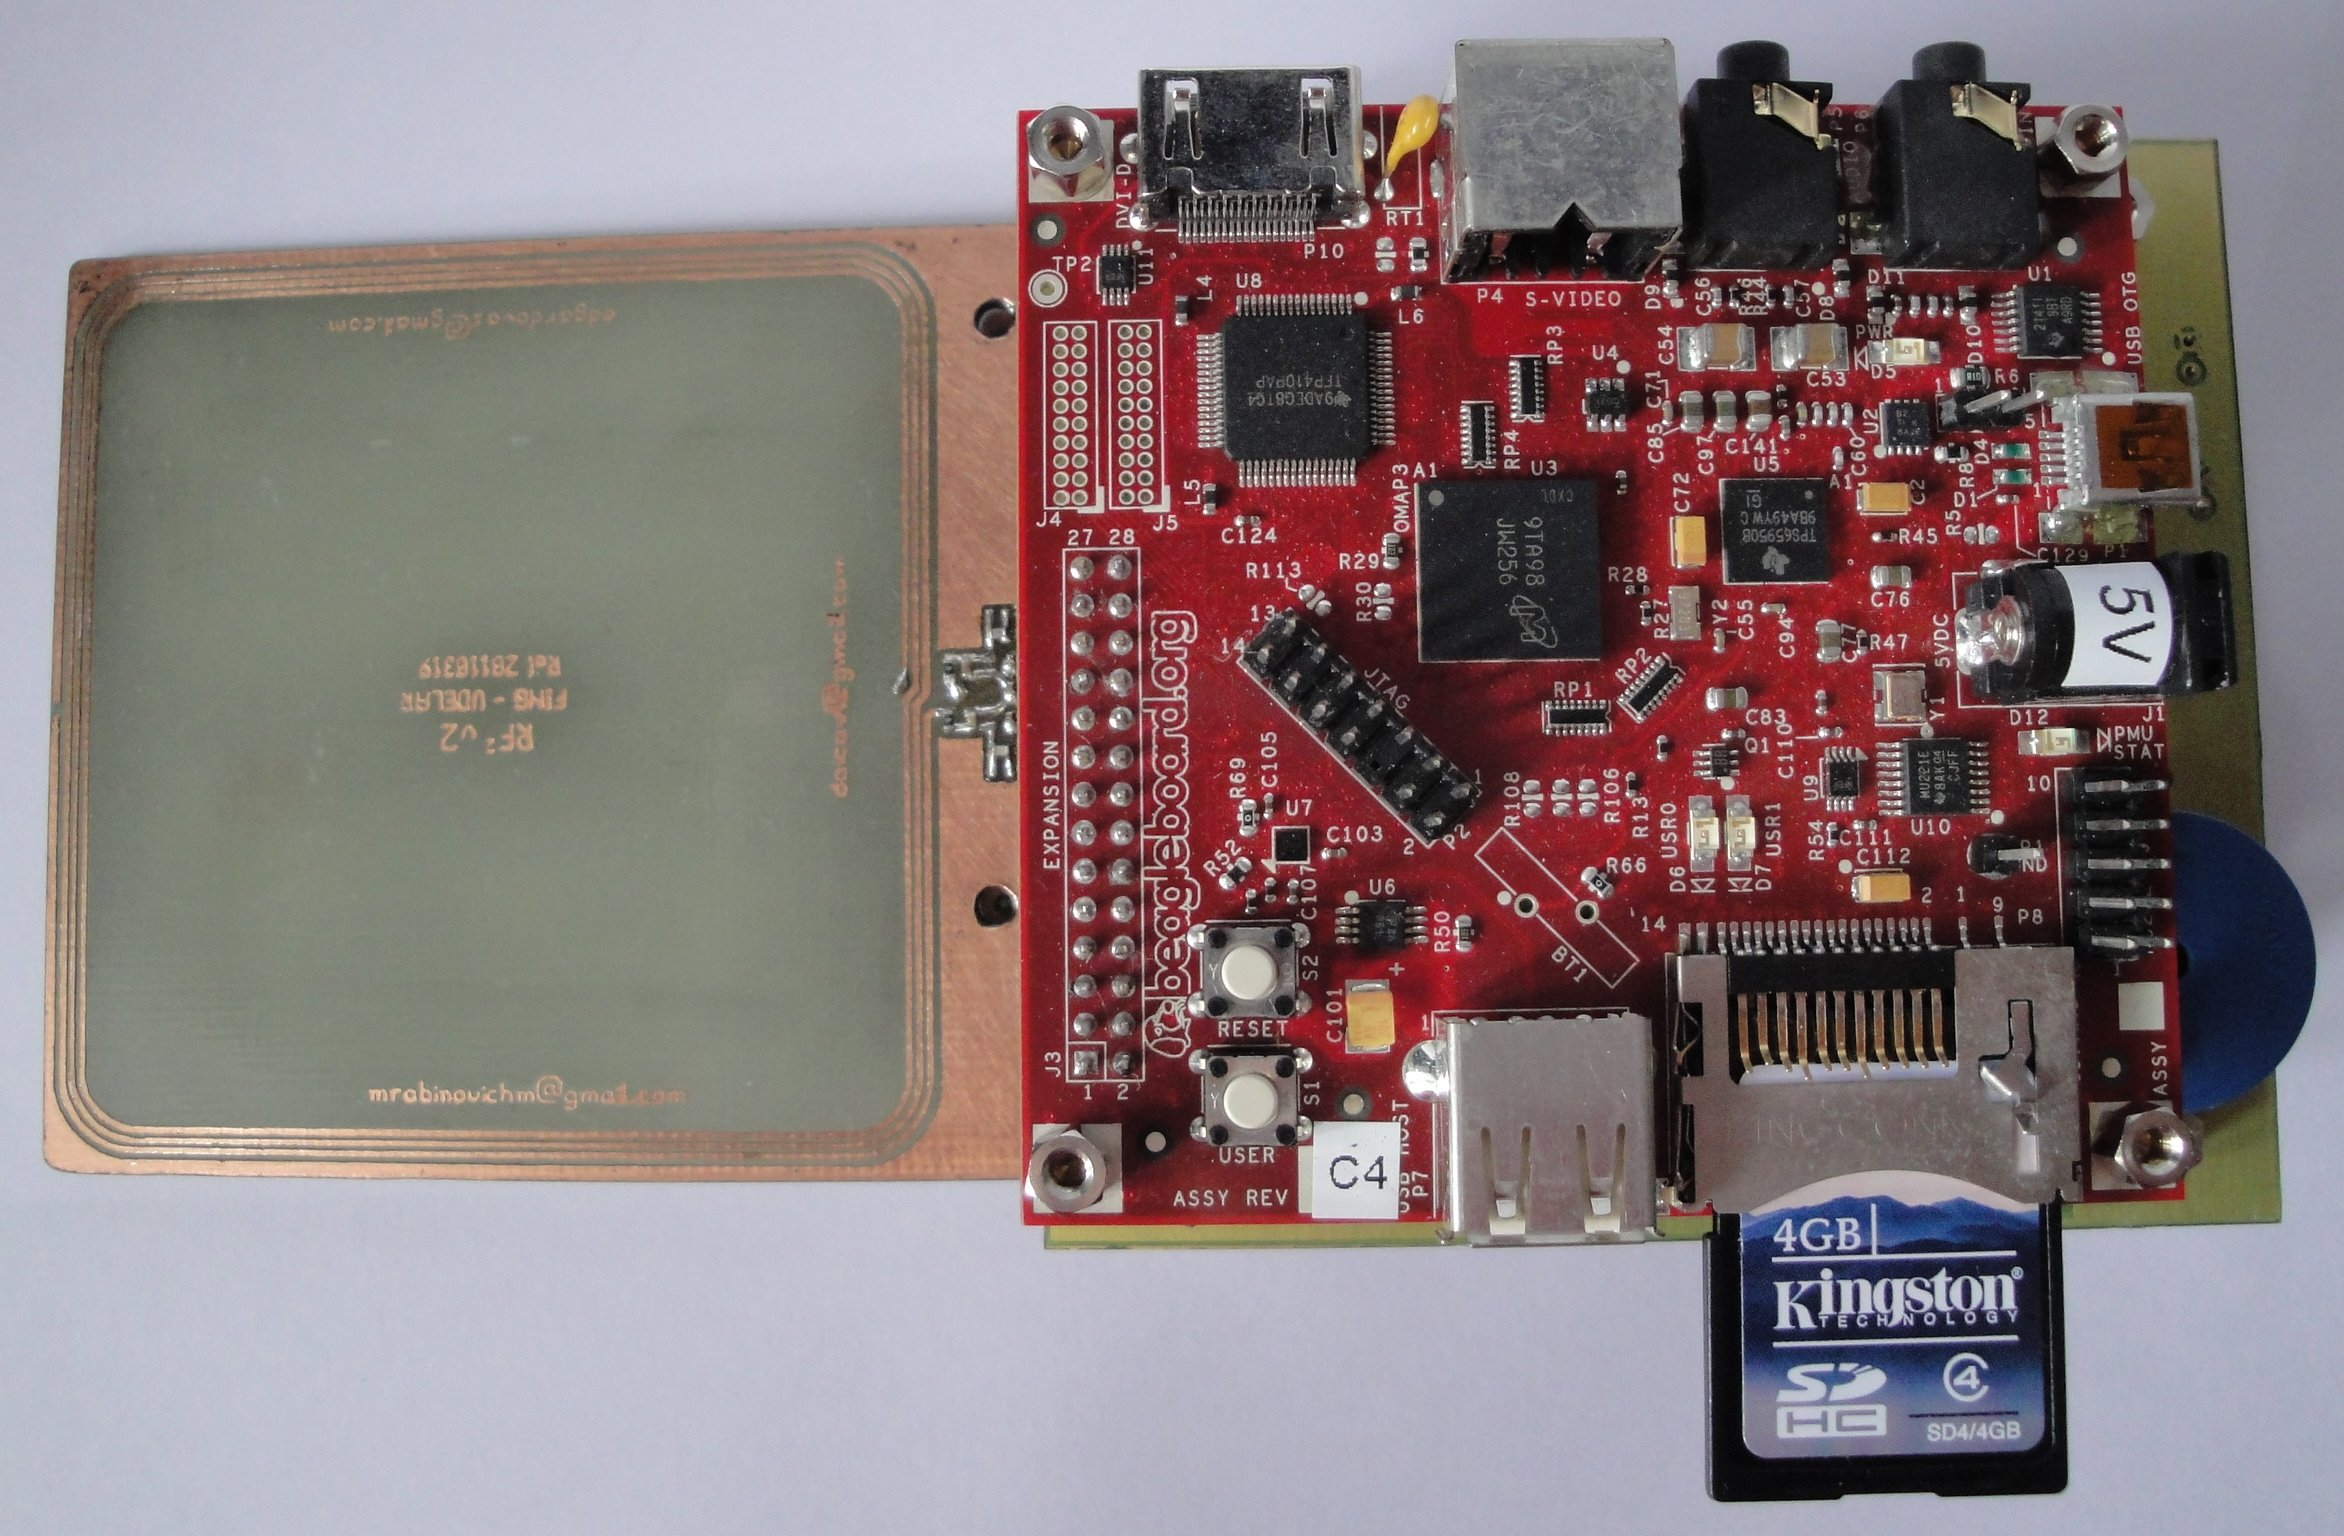
\includegraphics[scale=.13]{Imagenes/prototipo_b.jpg} }

  \caption{Vista anversa y reversa del prototipo}\label{protoFB}
\end{figure}

En cuanto al software, está basado en bibliotecas de código abierto que permiten desarrollar la aplicación que asegura el manejo del hardware y el funcionamiento de todo el sistema en conjunto.


\section{Funcionamiento general del prototipo}
Una vez que el prototipo RF$^{2}$ se encuentra operativo, el dispositivo despliega en el display el mensaje “Aproxime su tarjeta”, permaneciendo en dicho estado hasta que algún usuario acerque una tarjeta al lector/escritor RFID. 
En la primera transacción entre lector y tarjeta se obtiene el identificador único (UID) de ésta última, que será enviado al módulo de seguridad SAM (previa autenticación exitosa), para que a partir de éste, se generen las claves de acceso que permitan la lectura y escritura de la tarjeta RFID.
Mientras se lleva a cabo la operación, se despliega en el display el mensaje, “No retire su tarjeta” a la vez que el led amarillo es encendido para indicar precaución ya que se están procesando datos.
La siguiente acción a llevar a cabo es verificar que la tarjeta del usuario tenga saldo pendiente de acreditar, en caso afirmativo se indica al usuario el saldo a acreditar a través del display con el mensaje “Saldo a acreditar \$...”. Si todo fue exitoso, se borra el saldo transferido de la lista de saldos pendientes a acreditar para que no se transfiera saldo indefinidas veces.
A continuación se despliega en el display el nuevo monto almacenado en la tarjeta, “Su saldo es de \$...”, se enciende el led verde y se emite un pitido mediante el buzzer en señal que la operación fue satisfactoria.
Por último se muestran en el display los mensajes “Transacción finalizada”, “Gracias” y vuelve al inicio para comenzar un nuevo ciclo.

En caso que la tarjeta no tuviera saldo pendiente de acreditar, el prototipo RF$^{2}$ funciona en modo consulta y despliega en el display el saldo disponible en la tarjeta, “Su saldo es de \$...”, encendiendo el led verde y emitiendo un pitido, seguido de los mensajes “Transacción finalizada”, “Gracias” y vuelve al inicio para comenzar un nuevo ciclo.

En caso de ocurrir un error durante alguno de los pasos anteriores, ya sea porque
el usuario retiró la tarjeta en un momento inadecuado, o simplemente porque el prototipo RF$^{2}$
no logró leer o escribir la tarjeta en forma correcta, se enciende el led rojo, se emite un
doble pitido mediante el buzzer, y el display muestra el mensaje “Error, vuelva a intentarlo”,
acto seguido el ciclo vuelve a comenzar. 

\begin{figure}[H]
\centering
  \begin{center}
   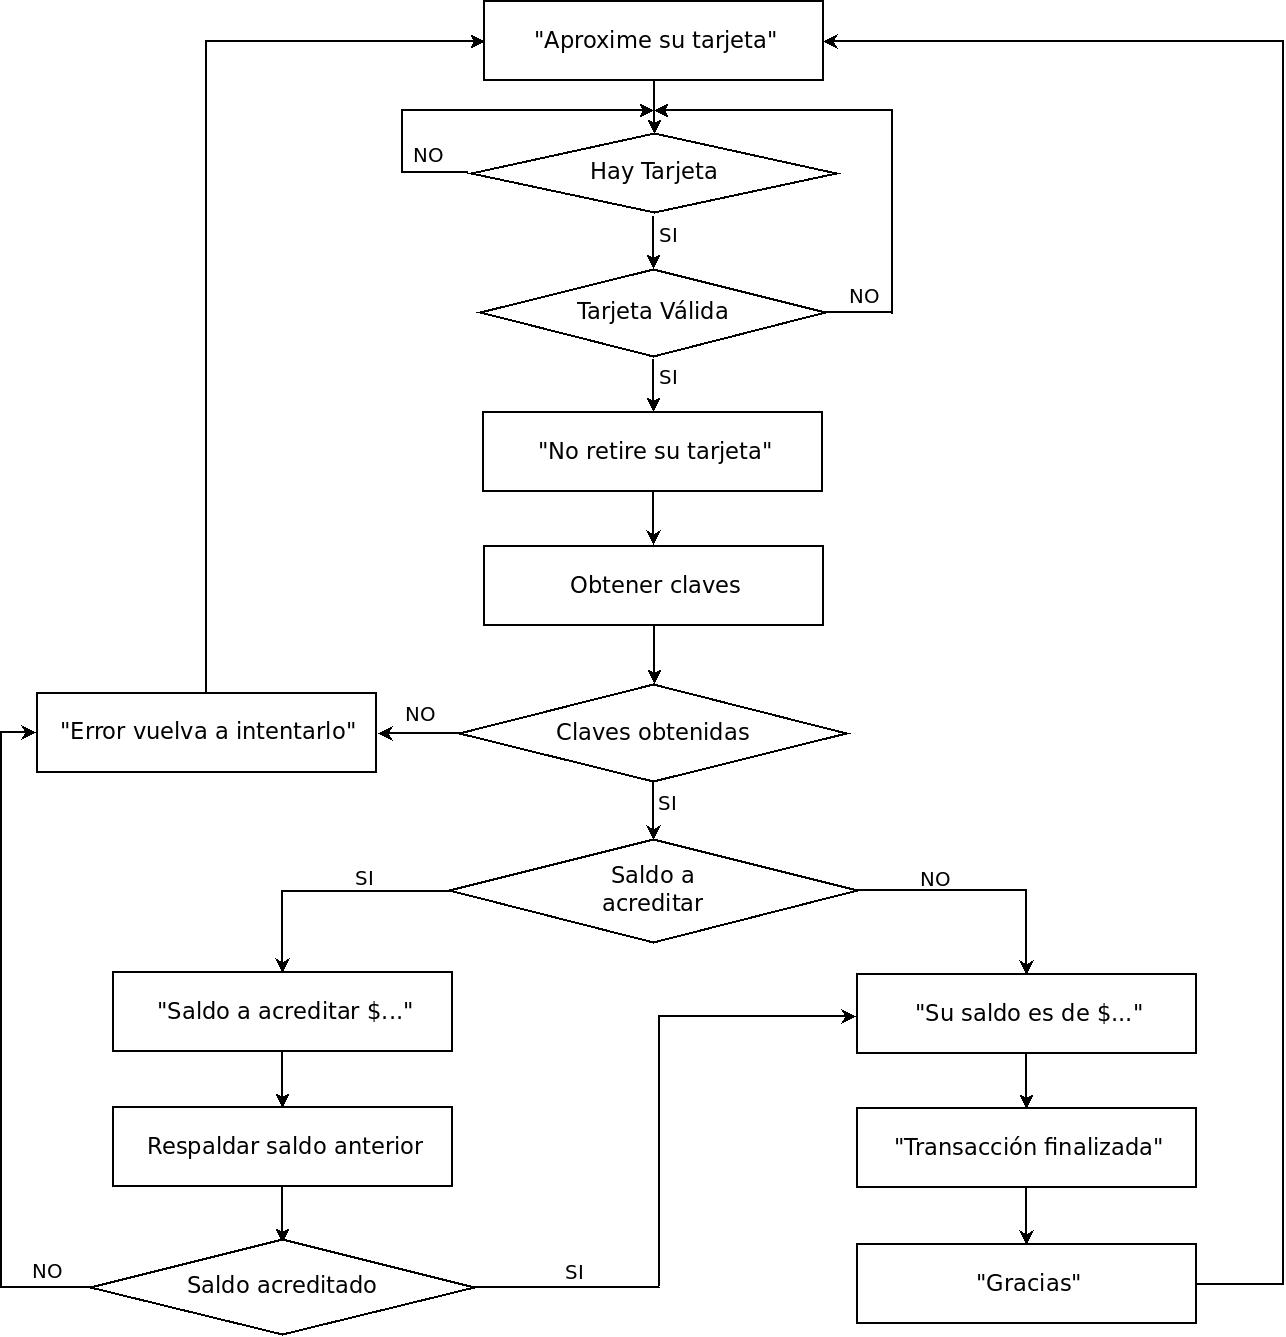
\includegraphics[scale=.35]{Imagenes/flujo.jpg}
  \end{center}
  \caption{Diagrama de flujo}\label{Fig:HW} 
\end{figure}
\chapter{Hardware}

%sección 4.1
\section{Arquitecturas estudiadas}\label{arqEst}
Se plantearon varias alternativas como posible solución. A medida que se encontraron limitantes o que no se cumplían los requerimientos exigidos, se fueron descartando dichas opciones.

A continuación se describen algunas de las arquitecturas consideradas:

\begin{itemize}
\item[1 -] OpenPCD + lector de tarjetas de contacto + display + buzzer + leds
\bigskip

\begin{figure}[H]
\centering
  \begin{center}
  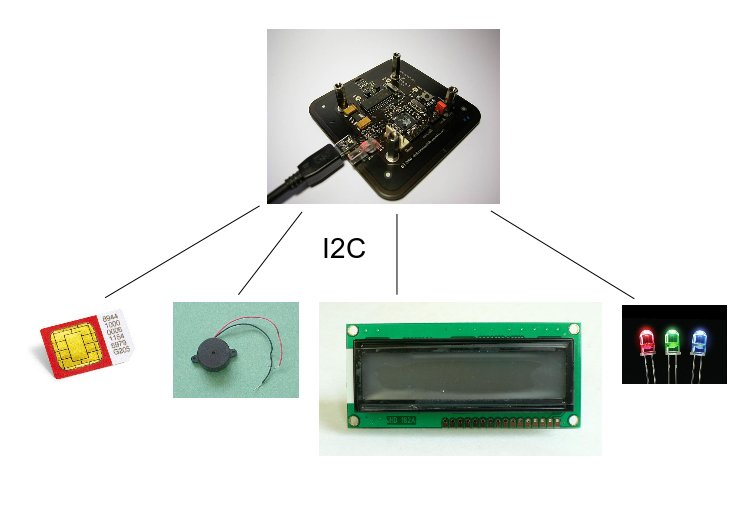
\includegraphics[scale=.4]{Imagenes/0.jpg} 
  \end{center}
  \caption{Solución considerada 1}\label{Fig:HW1} 
\end{figure}

\newpage
Al dispositivo OpenPCD, se conecta el resto del hardware a través de su único puerto de entrada/salida disponible que es de tipo I2C.

\bigskip
\item[2 -] SBC + OpenPCD + microcontrolador + lector de tarjetas de contacto + display + buzzer + leds
\bigskip

\begin{figure}[H]
\centering
  \begin{center}
  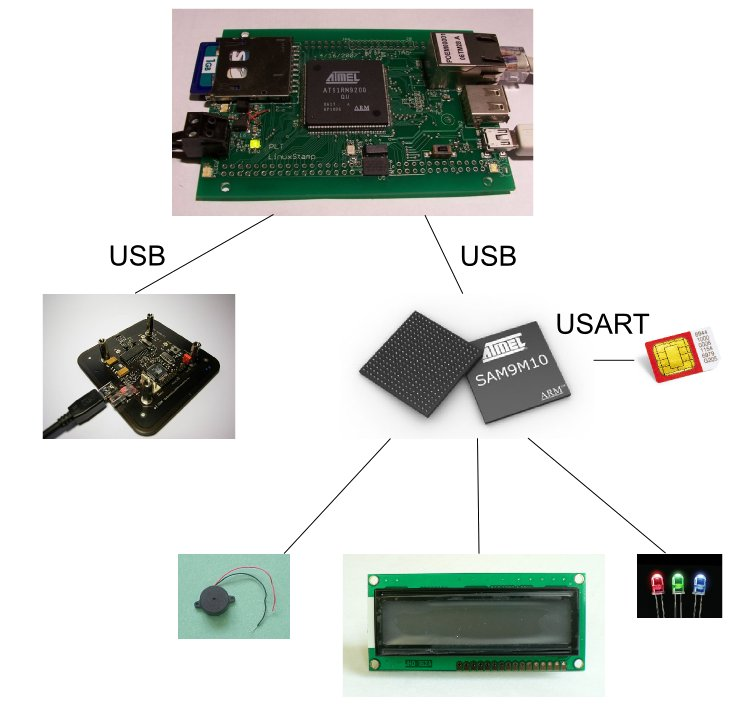
\includegraphics[scale=.3]{Imagenes/1.jpg} 
  \end{center}
  \caption{Solución considerada 2}\label{Fig:HW2} 
\end{figure}

Tanto el dispositivo OpenPCD como el microcontrolador se conectan directamente por USB a la SBC. El microcontrolador maneja el resto de los dispositivos (lector de tarjetas de contacto, display, buzzer y leds).

\bigskip
\item[3 -] SBC + OpenPCD + lector de tarjetas de contacto + display + buzzer + leds
\bigskip

\begin{figure}[H]
\centering
  \begin{center}
  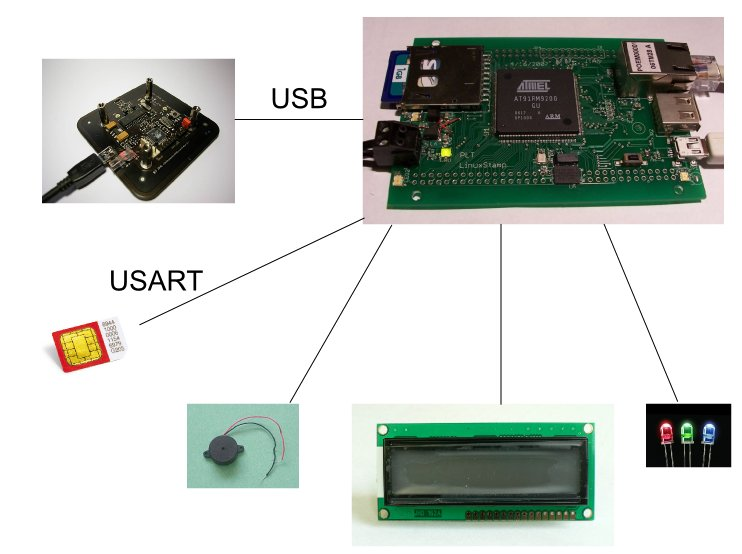
\includegraphics[scale=.25]{Imagenes/2.jpg} 
  \end{center}
  \caption{Solución considerada 3}\label{Fig:HW3} 
\end{figure}

El dispositivo OpenPCD se conecta por USB a la SBC. La SBC maneja los dispositivos (lector de tarjetas de contacto, display, buzzer y leds) a través de sus interfaces nativas.

\bigskip
\item[4 -] SBC + lector de tarjetas RFID + lector de tarjetas de contacto + display + buzzer + leds
\bigskip

\begin{figure}[H]
\centering
  \begin{center}
  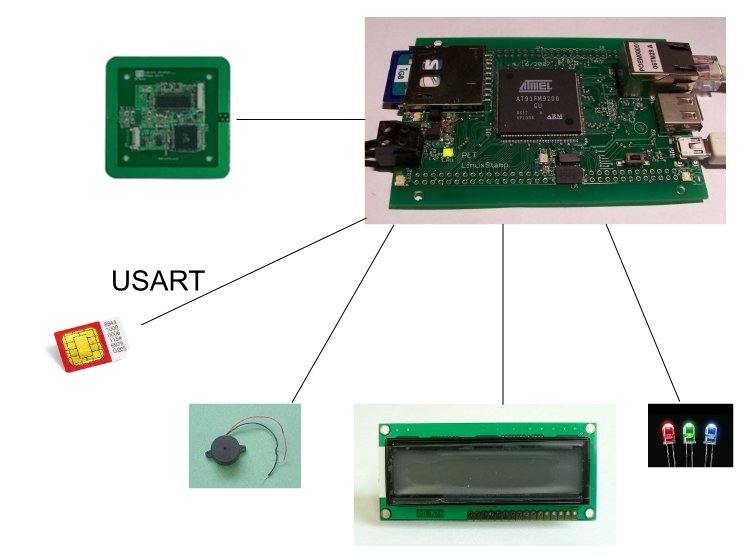
\includegraphics[scale=.25]{Imagenes/3.jpg} 
  \end{center}
  \caption{Solución considerada 4}\label{Fig:HW4} 
\end{figure}

Todos los periféricos se conectan a la SBC a través de sus interfaces nativas, esto incluye también el integrado CL RC632 de Philips \cite{RC632} (ver hoja de datos en el apéndice \ref{HD}). Se debe diseñar la antena para propagar la señal RF hacia las tarjetas.

\bigskip
\item[5 -] microcontrolador + lector de tarjetas RFID + lector de tarjetas de contacto + display + buzzer + leds
\bigskip

\begin{figure}[H]
\centering
  \begin{center}
  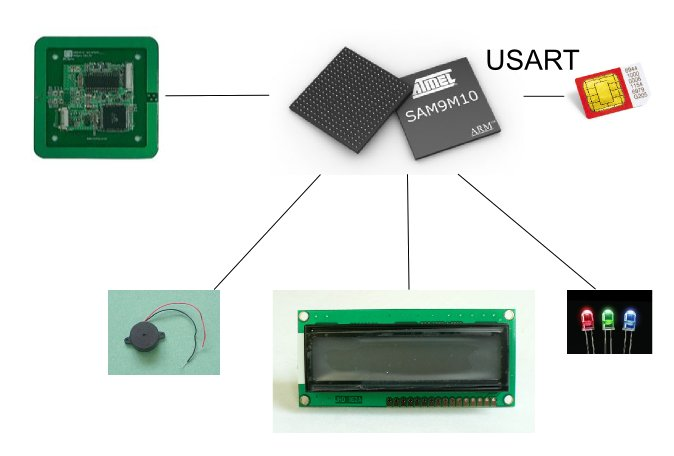
\includegraphics[scale=.25]{Imagenes/4.jpg} 
  \end{center}
  \caption{Solución considerada 5}\label{Fig:HW5} 
\end{figure}

Consta de un único PCB, que posee un microcontrolador como sistema central al cual se
conectan el resto de los dispositivos. Dicho PCB tiene incorporada la antena para la
propagación de RF.

\end{itemize}

\section{Arquitectura seleccionada}
En una primera instancia se pretendía utilizar únicamente el dispositivo OpenPCD (ver figura \ref{Fig:HW1}), ya que el mismo cuenta con un microcontrolador de la familia ARM, el AT91SAM7S128. Una vez estudiado se llegó a la conclusión que no permitía la instalación de un sistema operativo GNU/Linux, ya que el mismo precisa más de 4 MB de RAM para poder hacer algo útil. Otra desventaja encontrada fue que sólo tiene un puerto I2C como forma de conectar periféricos.

Surgió entonces la necesidad de usar una SBC como dispositivo capaz de ejecutar un sistema operativo y las aplicaciones necesarias para que el dispositivo cumpla con los requerimientos exigidos. El dispositivo OpenPCD pasaría entonces a cumplir la función de lector/escritor de tarjetas RFID (ver figuras \ref{Fig:HW2} y \ref{Fig:HW3}), conectado a la SBC a través de su puerto USB, mientras que para el resto de los periféricos se diseñaría un PCB que fuera capaz de ser conectado a la SBC a través de sus interfaces nativas. Esta arquitectura fue descartada por el incremento en el costo del proyecto.

Fue necesario entonces descartar el uso del dispositivo OpenPCD y dar lugar a un diseño propio del lector/escritor de tarjetas RFID (ver figura \ref{Fig:HW4}), utilizando para esto el integrado CL RC632 de Philips.

La última opción y la más ambiciosa, plantea el diseño completo de un PCB (ver figura \ref{Fig:HW5}) conteniendo un microcontrolador y memoria capaz de ejecutar un sistema operativo, los lectores de tarjetas, tanto de contacto como RFID, y el resto de los periféricos (display, leds, buzzer). Esta opción fue dejada de lado por entender que excedería los plazos de tiempo del proyecto.

Se pensó entonces en diseñar la arquitectura 4 indicada en la figura \ref{Fig:HW4}, SBC + lector de tarjetas RFID + lector de tarjeta de contacto + display + buzzer + leds, y dado que se cuenta con un OpenPCD, la opción 3 mostrada en la figura \ref{Fig:HW3}, SBC + OpenPCD + lector de tarjetas de contacto + display + buzzer + leds, se dejaría como arquitectura alternativa si no se alcanzaran buenos resultados con el lector/escritor de tarjetas RFID.

\bigskip
Luego de estudiar ventajas y desventajas de las arquitecturas planteadas, se eligió la indicada en el ítem 4 en la sección \ref{arqEst}, que es la que más se adaptó a los requerimientos necesarios:

\begin{itemize}
\item SBC +  lector de tarjetas RFID + lector de tarjeta de contacto + display + buzzer + leds
\end{itemize}

En la figura \ref{Fig:HW_GRAL} se muestra un diagrama de bloques correspondiente a la arquitectura seleccionada:

\begin{figure}[H]
\centering
  \begin{center}
  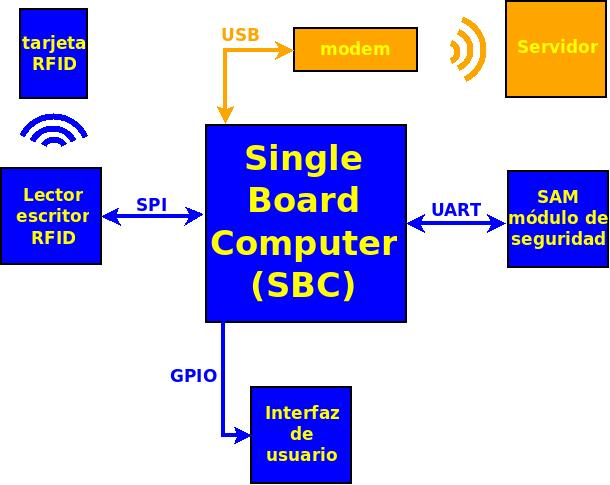
\includegraphics[scale=.5]{Imagenes/diagrama_rf2.jpg} 
  \end{center}
  \caption{Diagrama de bloques de la arquitectura seleccionada}\label{Fig:HW_GRAL} 
\end{figure}


Los bloques oscuros serán implementados, no así los claros.

\bigskip
Como se mencionó en el punto \ref{2.2}, el bloque de la figura \ref{Fig:HW_GRAL} referente al módulo de seguridad, no está operativo en la aplicación final. 
La comunicación con un servidor no está implementada por quedar fuera del alcance del proyecto.

\newpage
\section{Elecci\'on de hardware}

\subsection{SBC}
En primera instancia se confeccionó una lista con posibles candidatas de SBC disponibles
en el mercado internacional, teniendo en cuenta factores como: precio, puertos de I/O, memoria RAM, memoria Flash, puertos USB, soporte para GNU/Linux, entre otros.
Se definieron una serie de requisitos mínimos necesarios para seleccionar de la lista la SBC que más se adecuara a la arquitectura definida.
Para la comunicación con el resto de los módulos será necesario: una interfaz UART para el módulo de seguridad (SAM); una interfaz SPI para el módulo lector/escritor RFID (CL RC632 de Philips); 20 GPIO para display, leds, buzzer, otros; 1 USB host previendo una futura conexión de un modem 3G (intercambio de datos con un servidor). En cuanto a la memoria disponible, tomando como referencia el AFE, debe ser de 32 MB de RAM y 8 MB de flash para un funcionamiento aceptable. Es conveniente, pensando a futuro, que el procesador trabaje a una frecuencia no menor a 200 MHz.
Dado el presupuesto estimado para el proyecto, el precio no debe superar los 150 dólares en origen.
Como requisito adicional se exigió que existiera un foro actualizado y soporte técnico que permitiera evacuar dudas.


Aplicados los requisitos mínimos a la lista previamente confeccionada de SBC candidatas, se optó por dos: GESBC-9G20 \cite{9G20} y Hawkboard \cite{Hawk}.
En cuanto a la primera opción, GESBC-9G20, los fabricantes no respondieron consultas, por tanto se descartó. Se optó entonces por la segunda opción, Hawkboard, puesto que respondieron a las consultas en tiempos razonables y se logró evacuar dudas desde el foro.


Luego de comprar dos Hawkboard, ambas resultaron defectuosas a nivel de hardware, después de varios meses de pruebas sin resultados y sin respuestas concretas por parte del proveedor y fabricante y con la intención de cumplir con los plazos del proyecto, se optó por utilizar una SBC (Beagleboard \cite{Beagle}) que se consiguió en préstamo por medio del INCO. Esta SBC cumplió con los requisitos mínimos, aunque en ese momento tenía un costo del doble de la Hawkboard, teniéndose que diseñar un módulo hardware adicional.
Finalmente, la SBC seleccionada para trabajar fue la Beagleboard rev.C4.

Las características generales de la BeagleBoard son: cuenta con un procesador \\
OMAP3530 de 720 MHz con arquitectura ARM. Posee  memoria NAND-flash de 256 MB y memoria ROM de igual tamaño. Tiene una ranura adicional para extender la memoria a través de una memoria SD. Entre otras cosas cuenta con un puerto USB OTG, un puerto USB host, un bloque de expansión de 28 pines (con señales a 1,8 Volt), puerto JTAG, conector RS232, etc.\\
En lo que respecta a la potencia disipada, la Beagleboard tiene un consumo de pico de 2W, y un consumo promedio de 560mW \cite{consumo1} \cite{consumo2}.

\begin{figure}[H]
  \centering
  \subfigure[Vista anversa de la SBC]{\label{sbcF}
  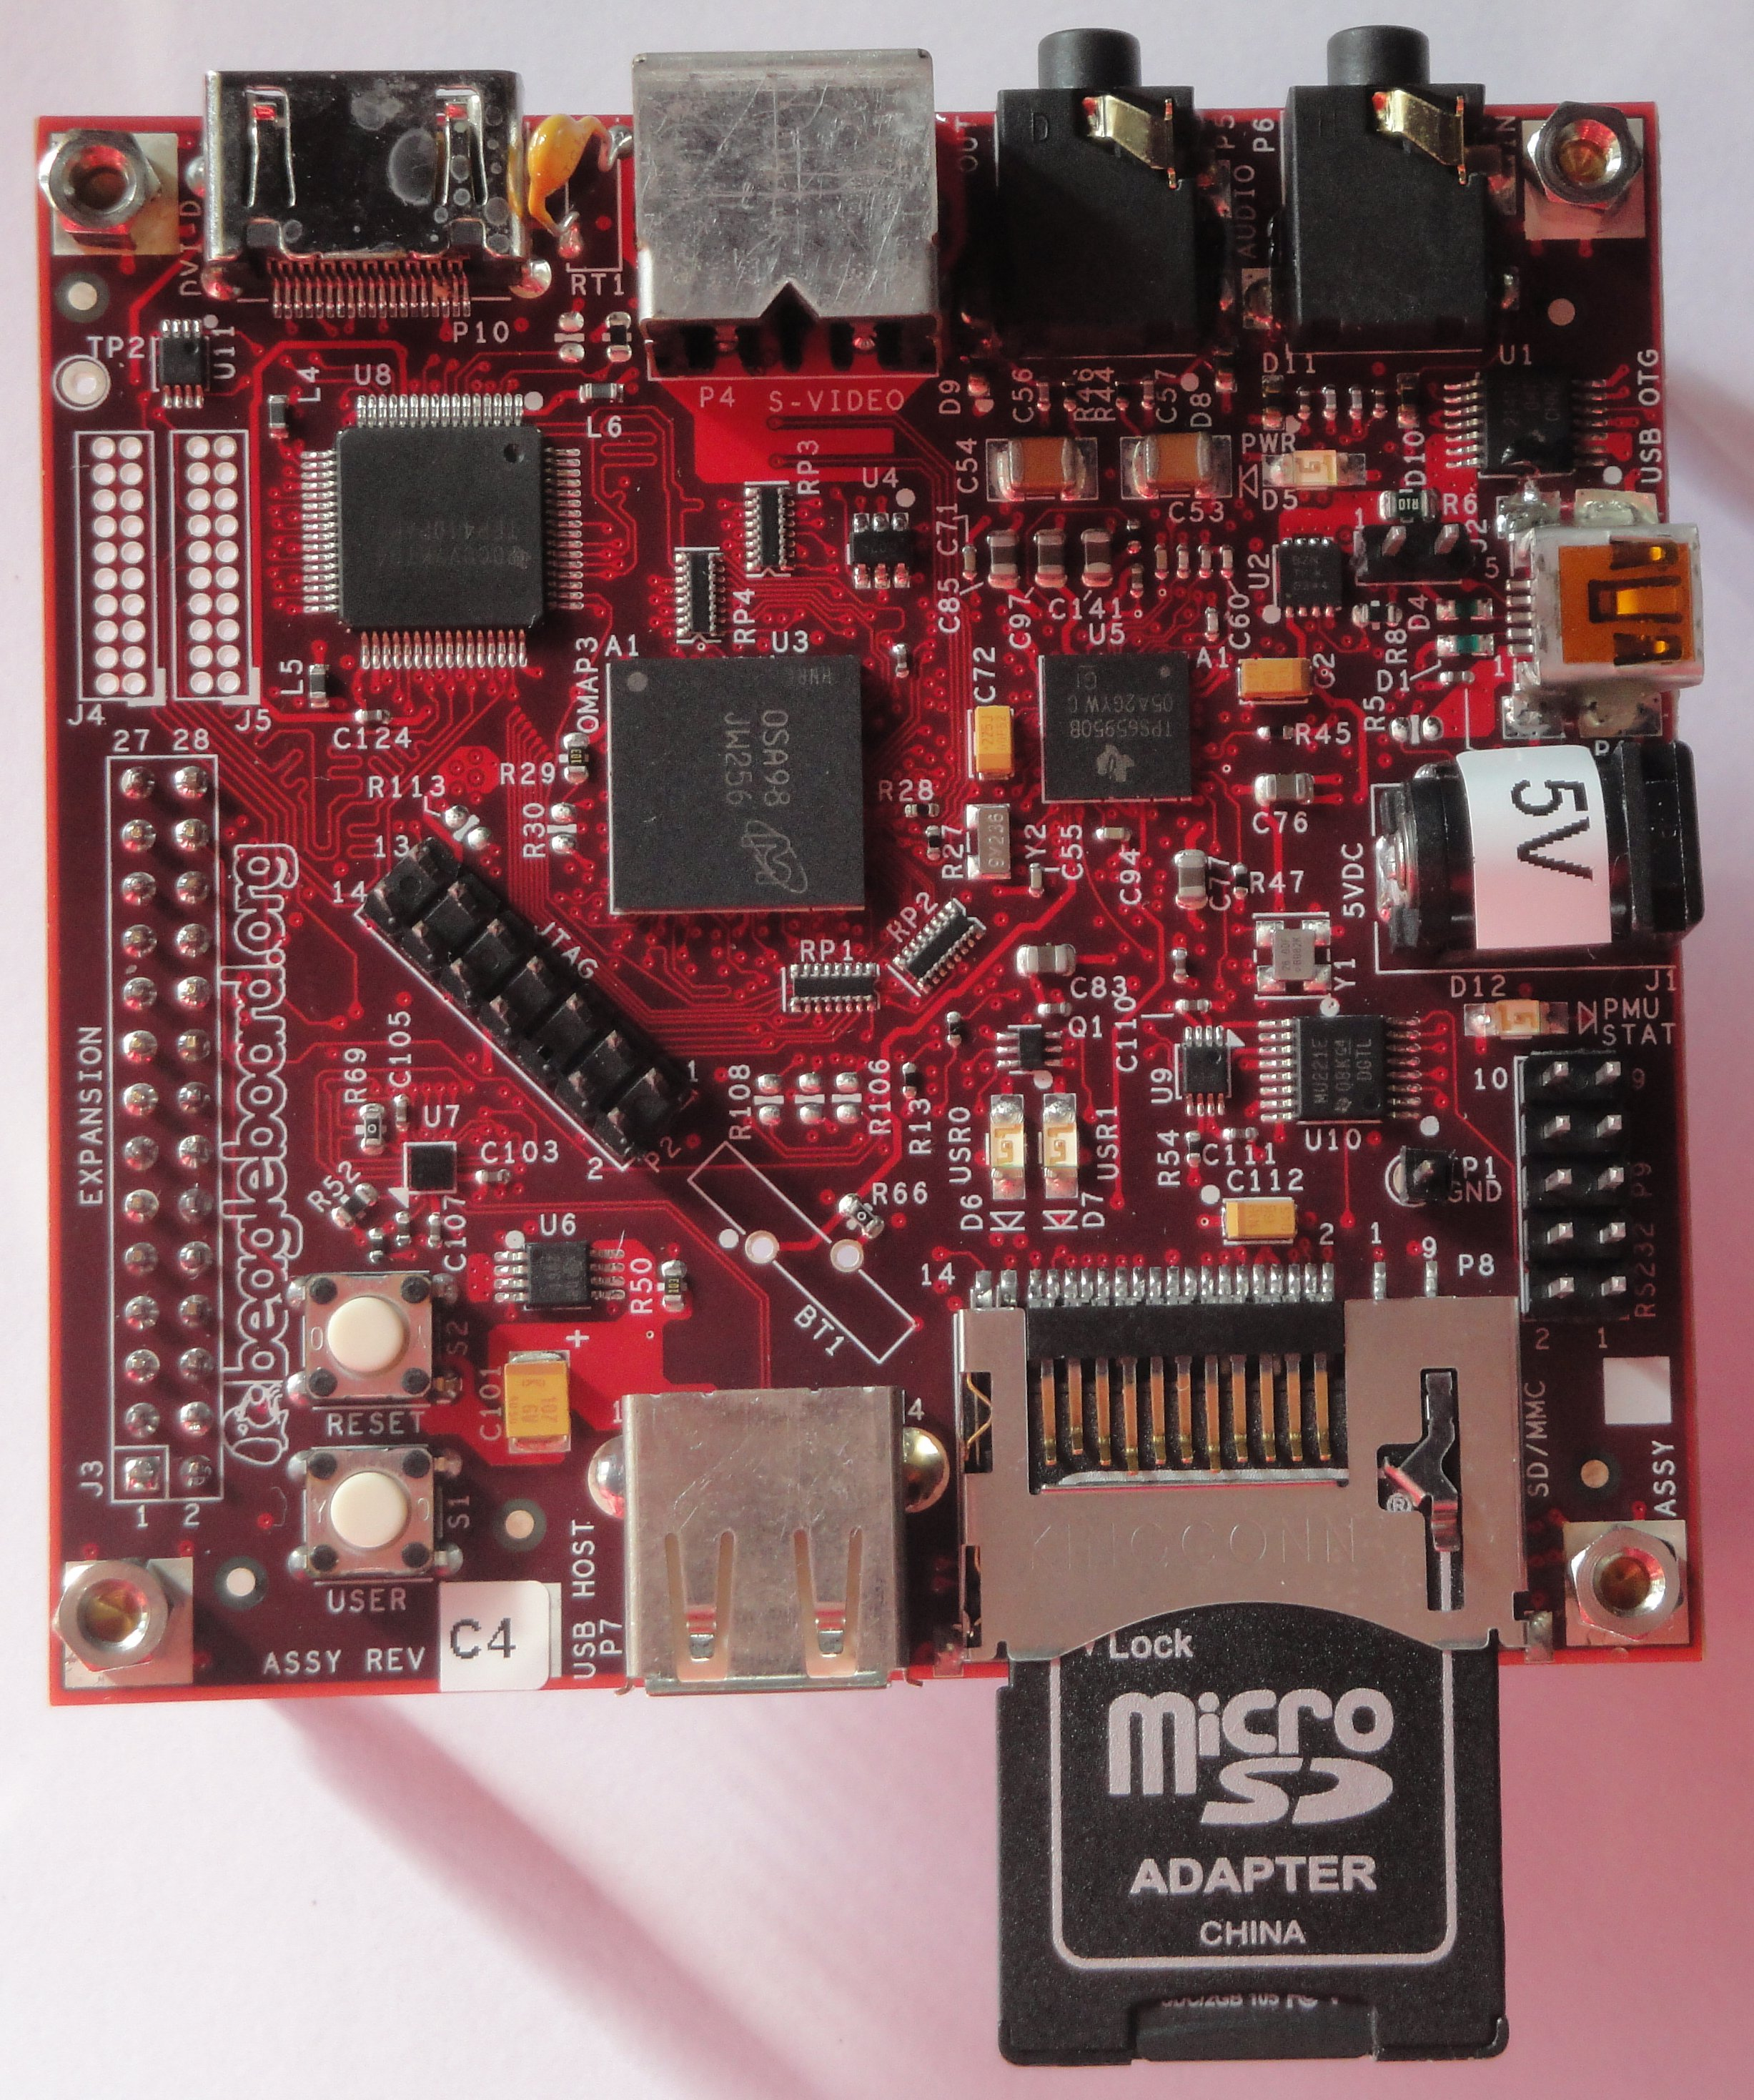
\includegraphics[scale=.08]{Imagenes/SBC_f.jpg} } 
  \subfigure[Vista reversa de la SBC]{\label{sbcB} 
  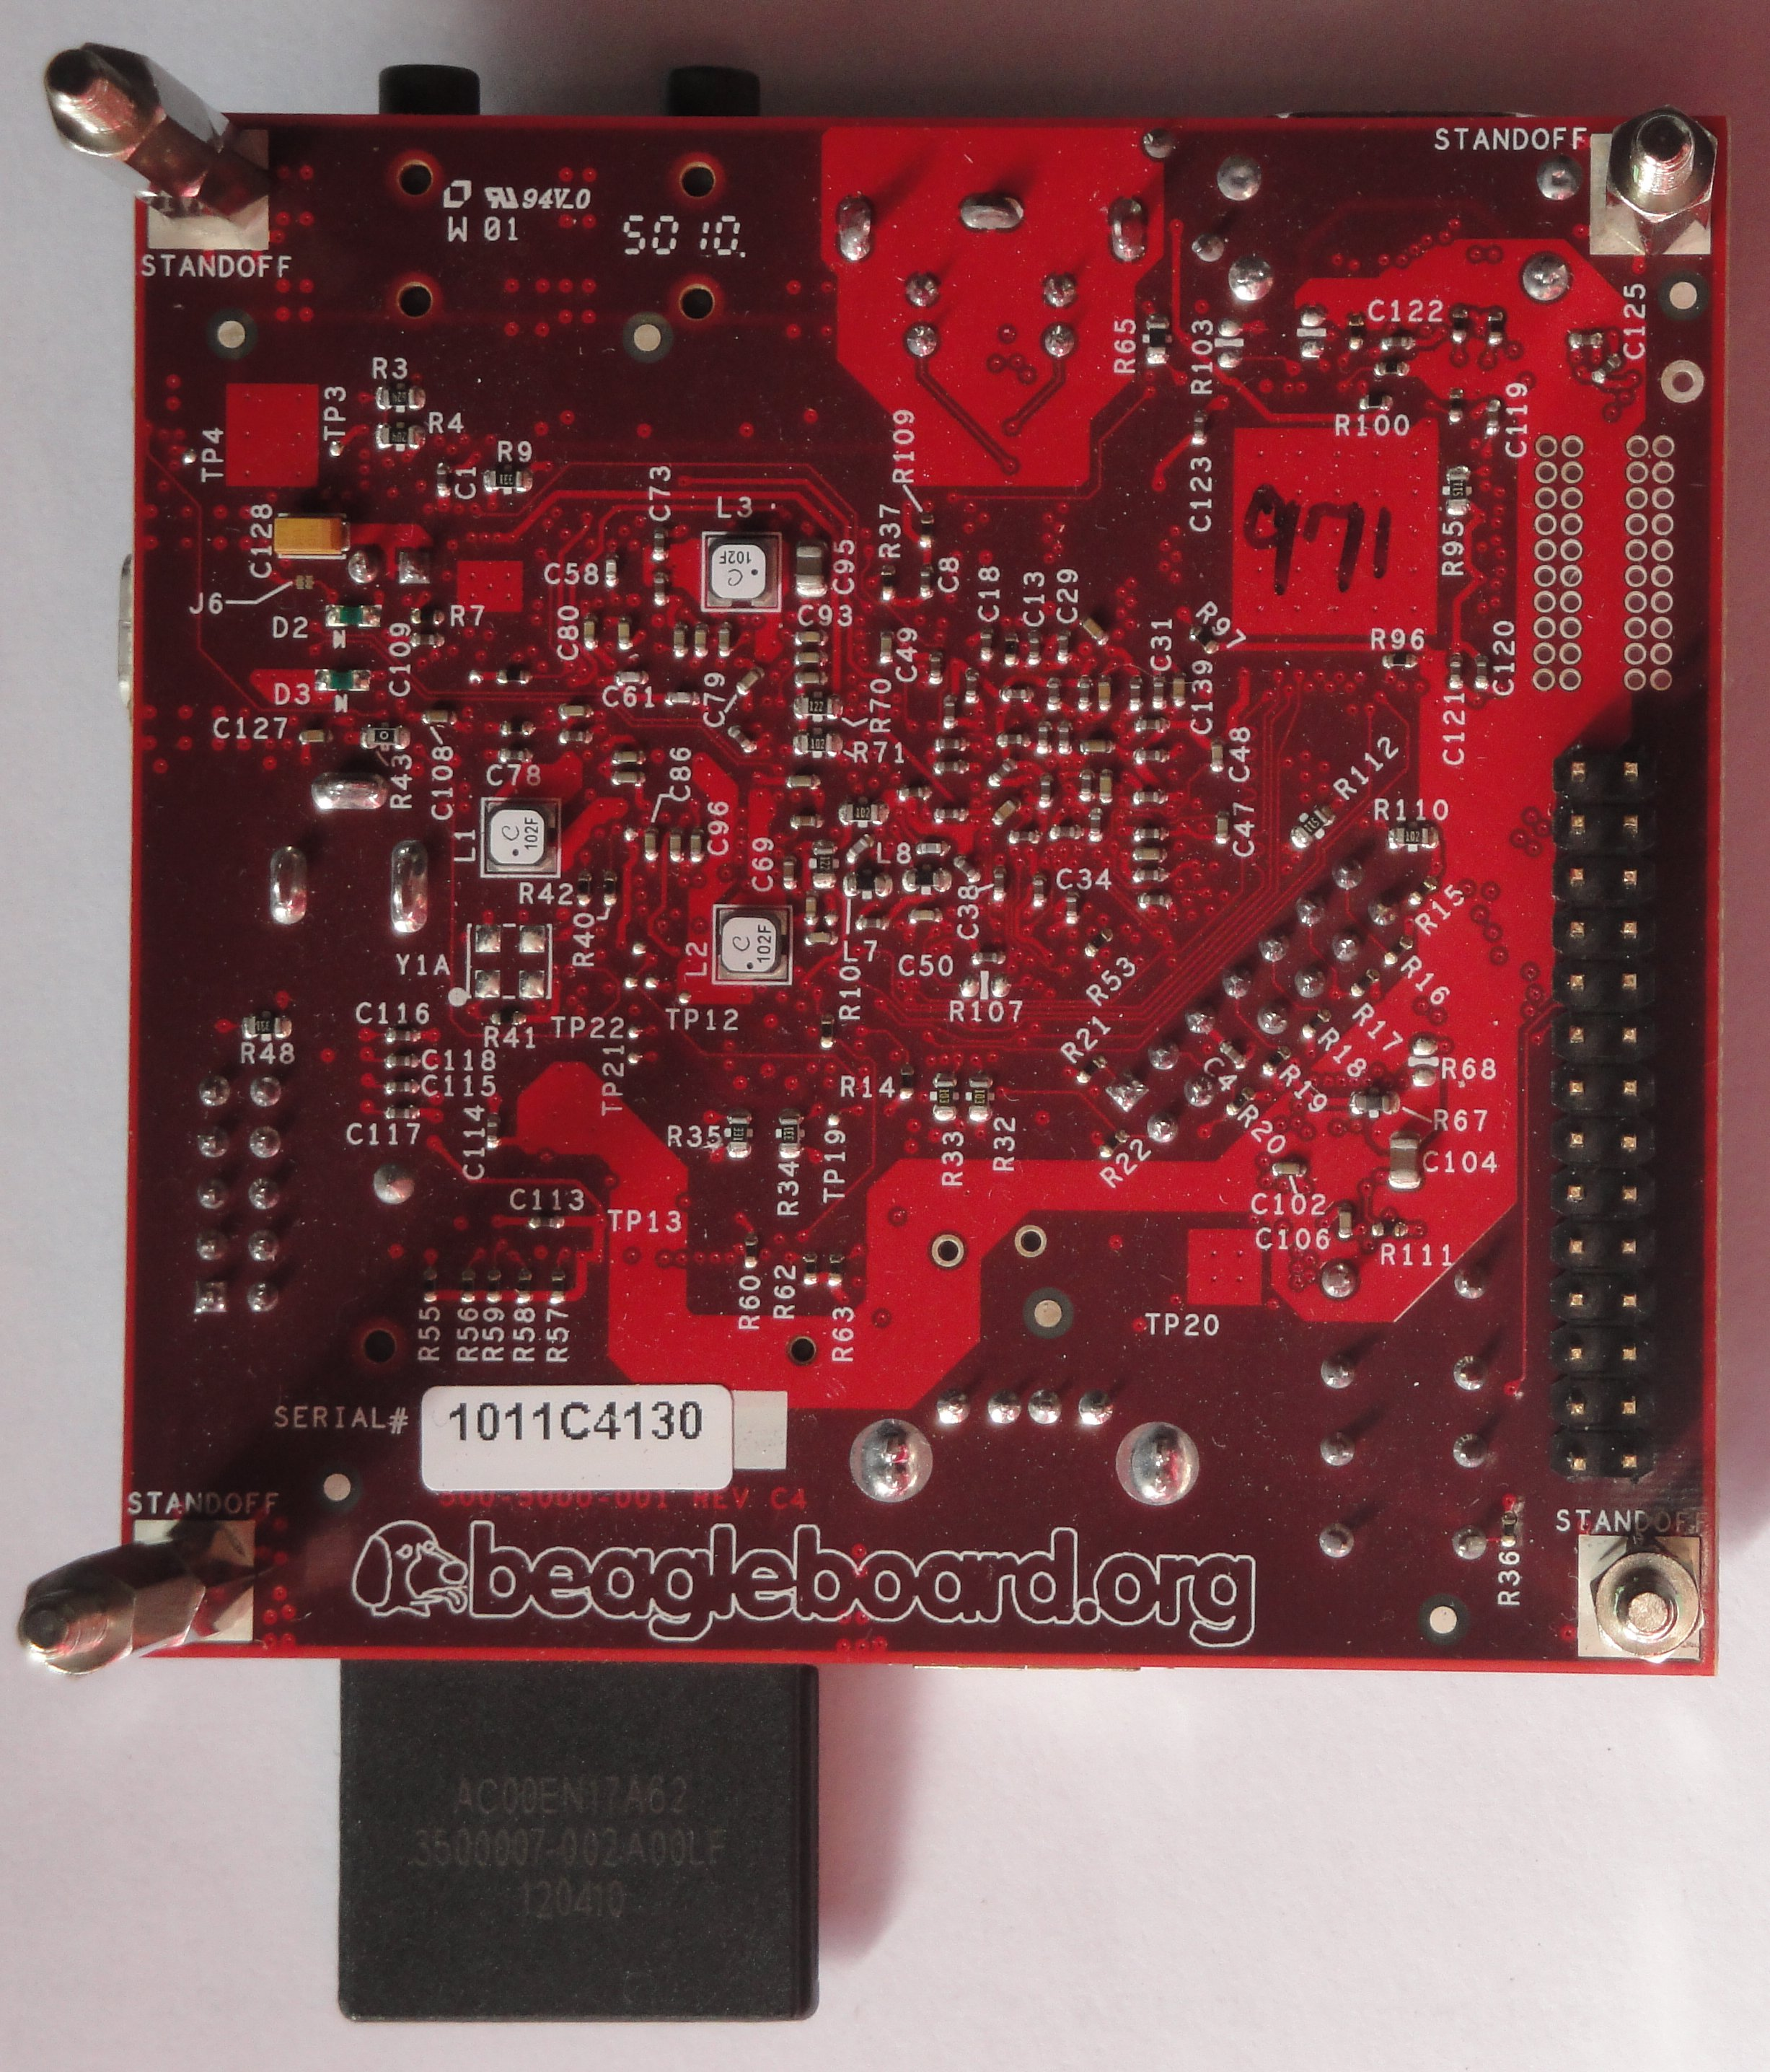
\includegraphics[scale=.08]{Imagenes/SBC_b.jpg} }

  \caption{Vista anversa y reversa de la SBC}\label{sbcFB}
\end{figure}


\subsection{VLT - Conversor de Voltajes}
Este módulo no fue tenido en cuenta en la primera etapa del diseño de la arquitectura hardware, sino que surge como necesidad debido al cambio de SBC. Como consecuencia de lo anterior se vio la ventaja de incorporar una placa que permite la conexión entre la SBC y el resto del hardware, el cual puede permanecer inalterado por más que no ocurra lo mismo con la SBC, ya que ésta puede cambiar de versión o dejar de fabricarse en un breve lapso de tiempo. El único elemento a cambiar sería entonces la placa VLT, que es más simple y barata de fabricar que las restantes partes.
La placa de circuito impreso VLT consta básicamente de dos conectores, uno de ellos permite la conexión con la Beagleboard y el otro la conexión con el restante hardware el cual se encuentra intergrado en un PCB llamdo SCUI. Ambos conectores no se encuentran directamente interconectados entre sí a través de pistas, pues para el caso particular de Beagleboard fue necesario incorporar conversores de tensión que permitieran el traslado del nivel de tensión desde 1,8 Volt que usa esta SBC, a las tensiones con las que operan los periféricos, ya sea 3,3 o 5 Volt.
El último elemento, no menos importante, es un regulador de tensión LDO que permite generar 3,3 Volt a partir de la fuente de tensión de 5 Volt de la propia Beagleboard.

Por más detalles ver esquemático en la figura \ref{Fig:VLT}.

\begin{figure}[H]
  \centering
  \subfigure[Vista anversa de la SBC]{\label{vltF}
  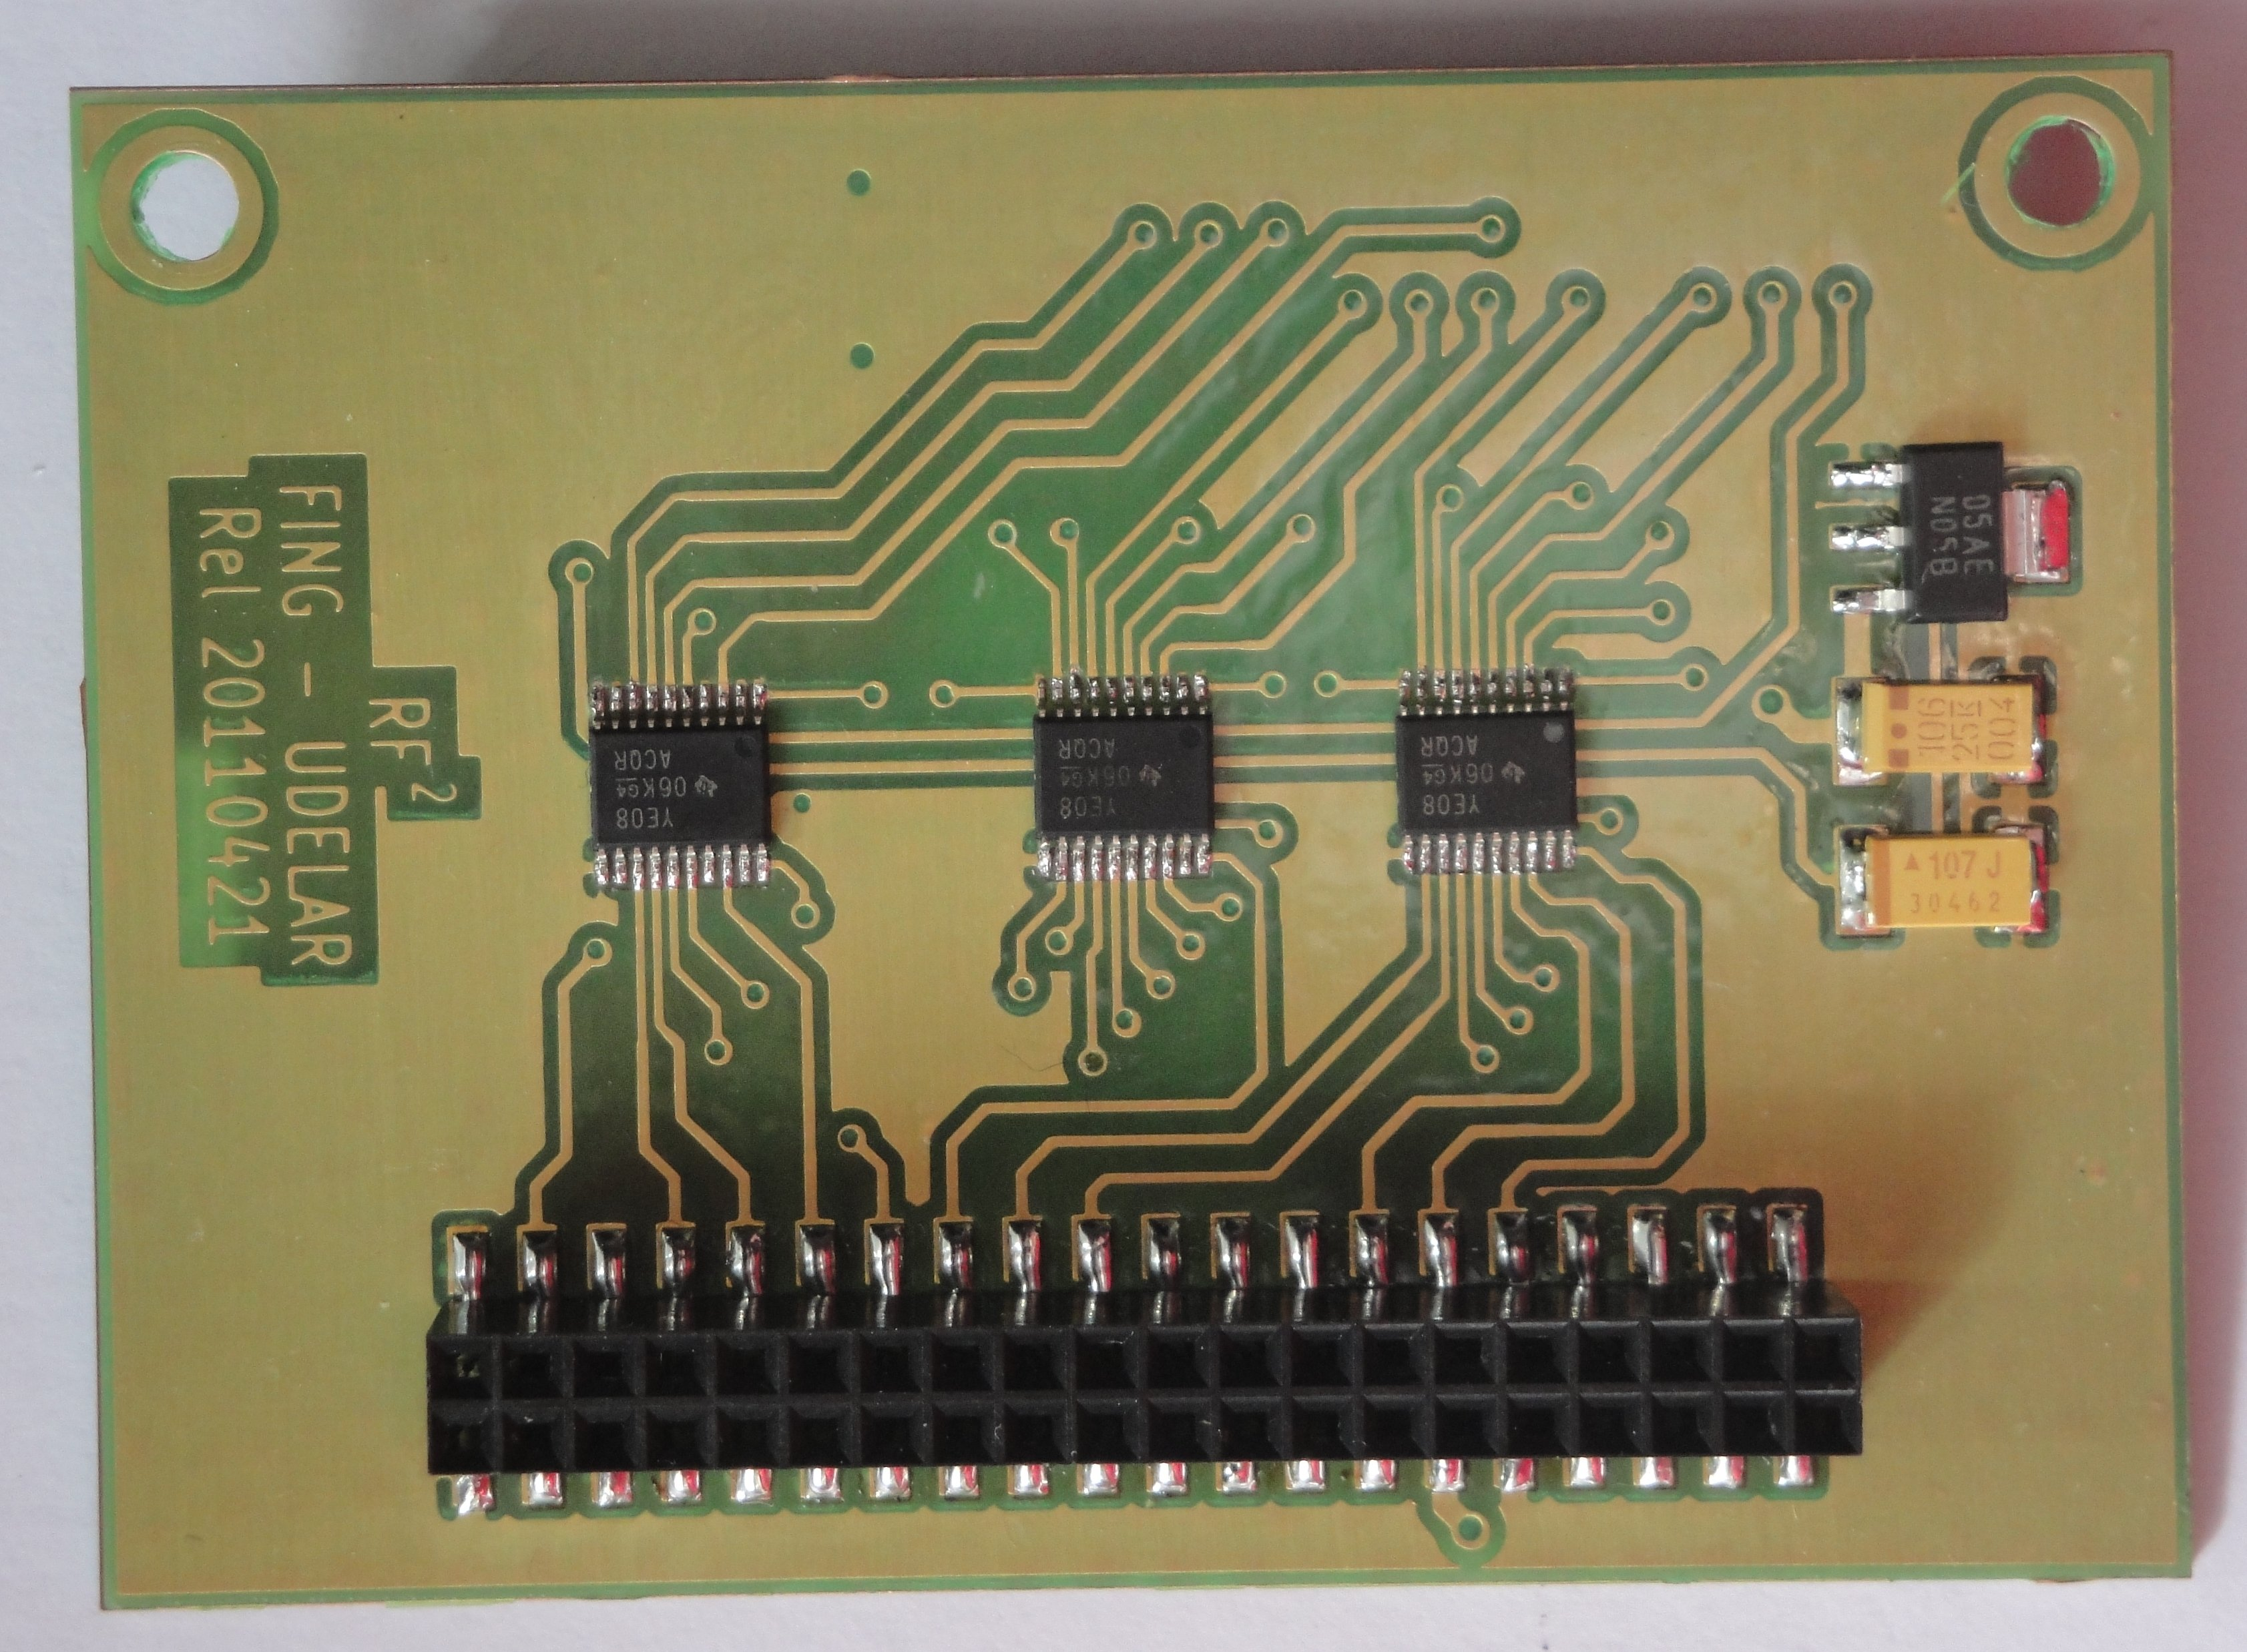
\includegraphics[scale=.08, angle=90]{Imagenes/VLT_f.jpg} } 
  \subfigure[Vista reversa de la SBC]{\label{vltB} 
  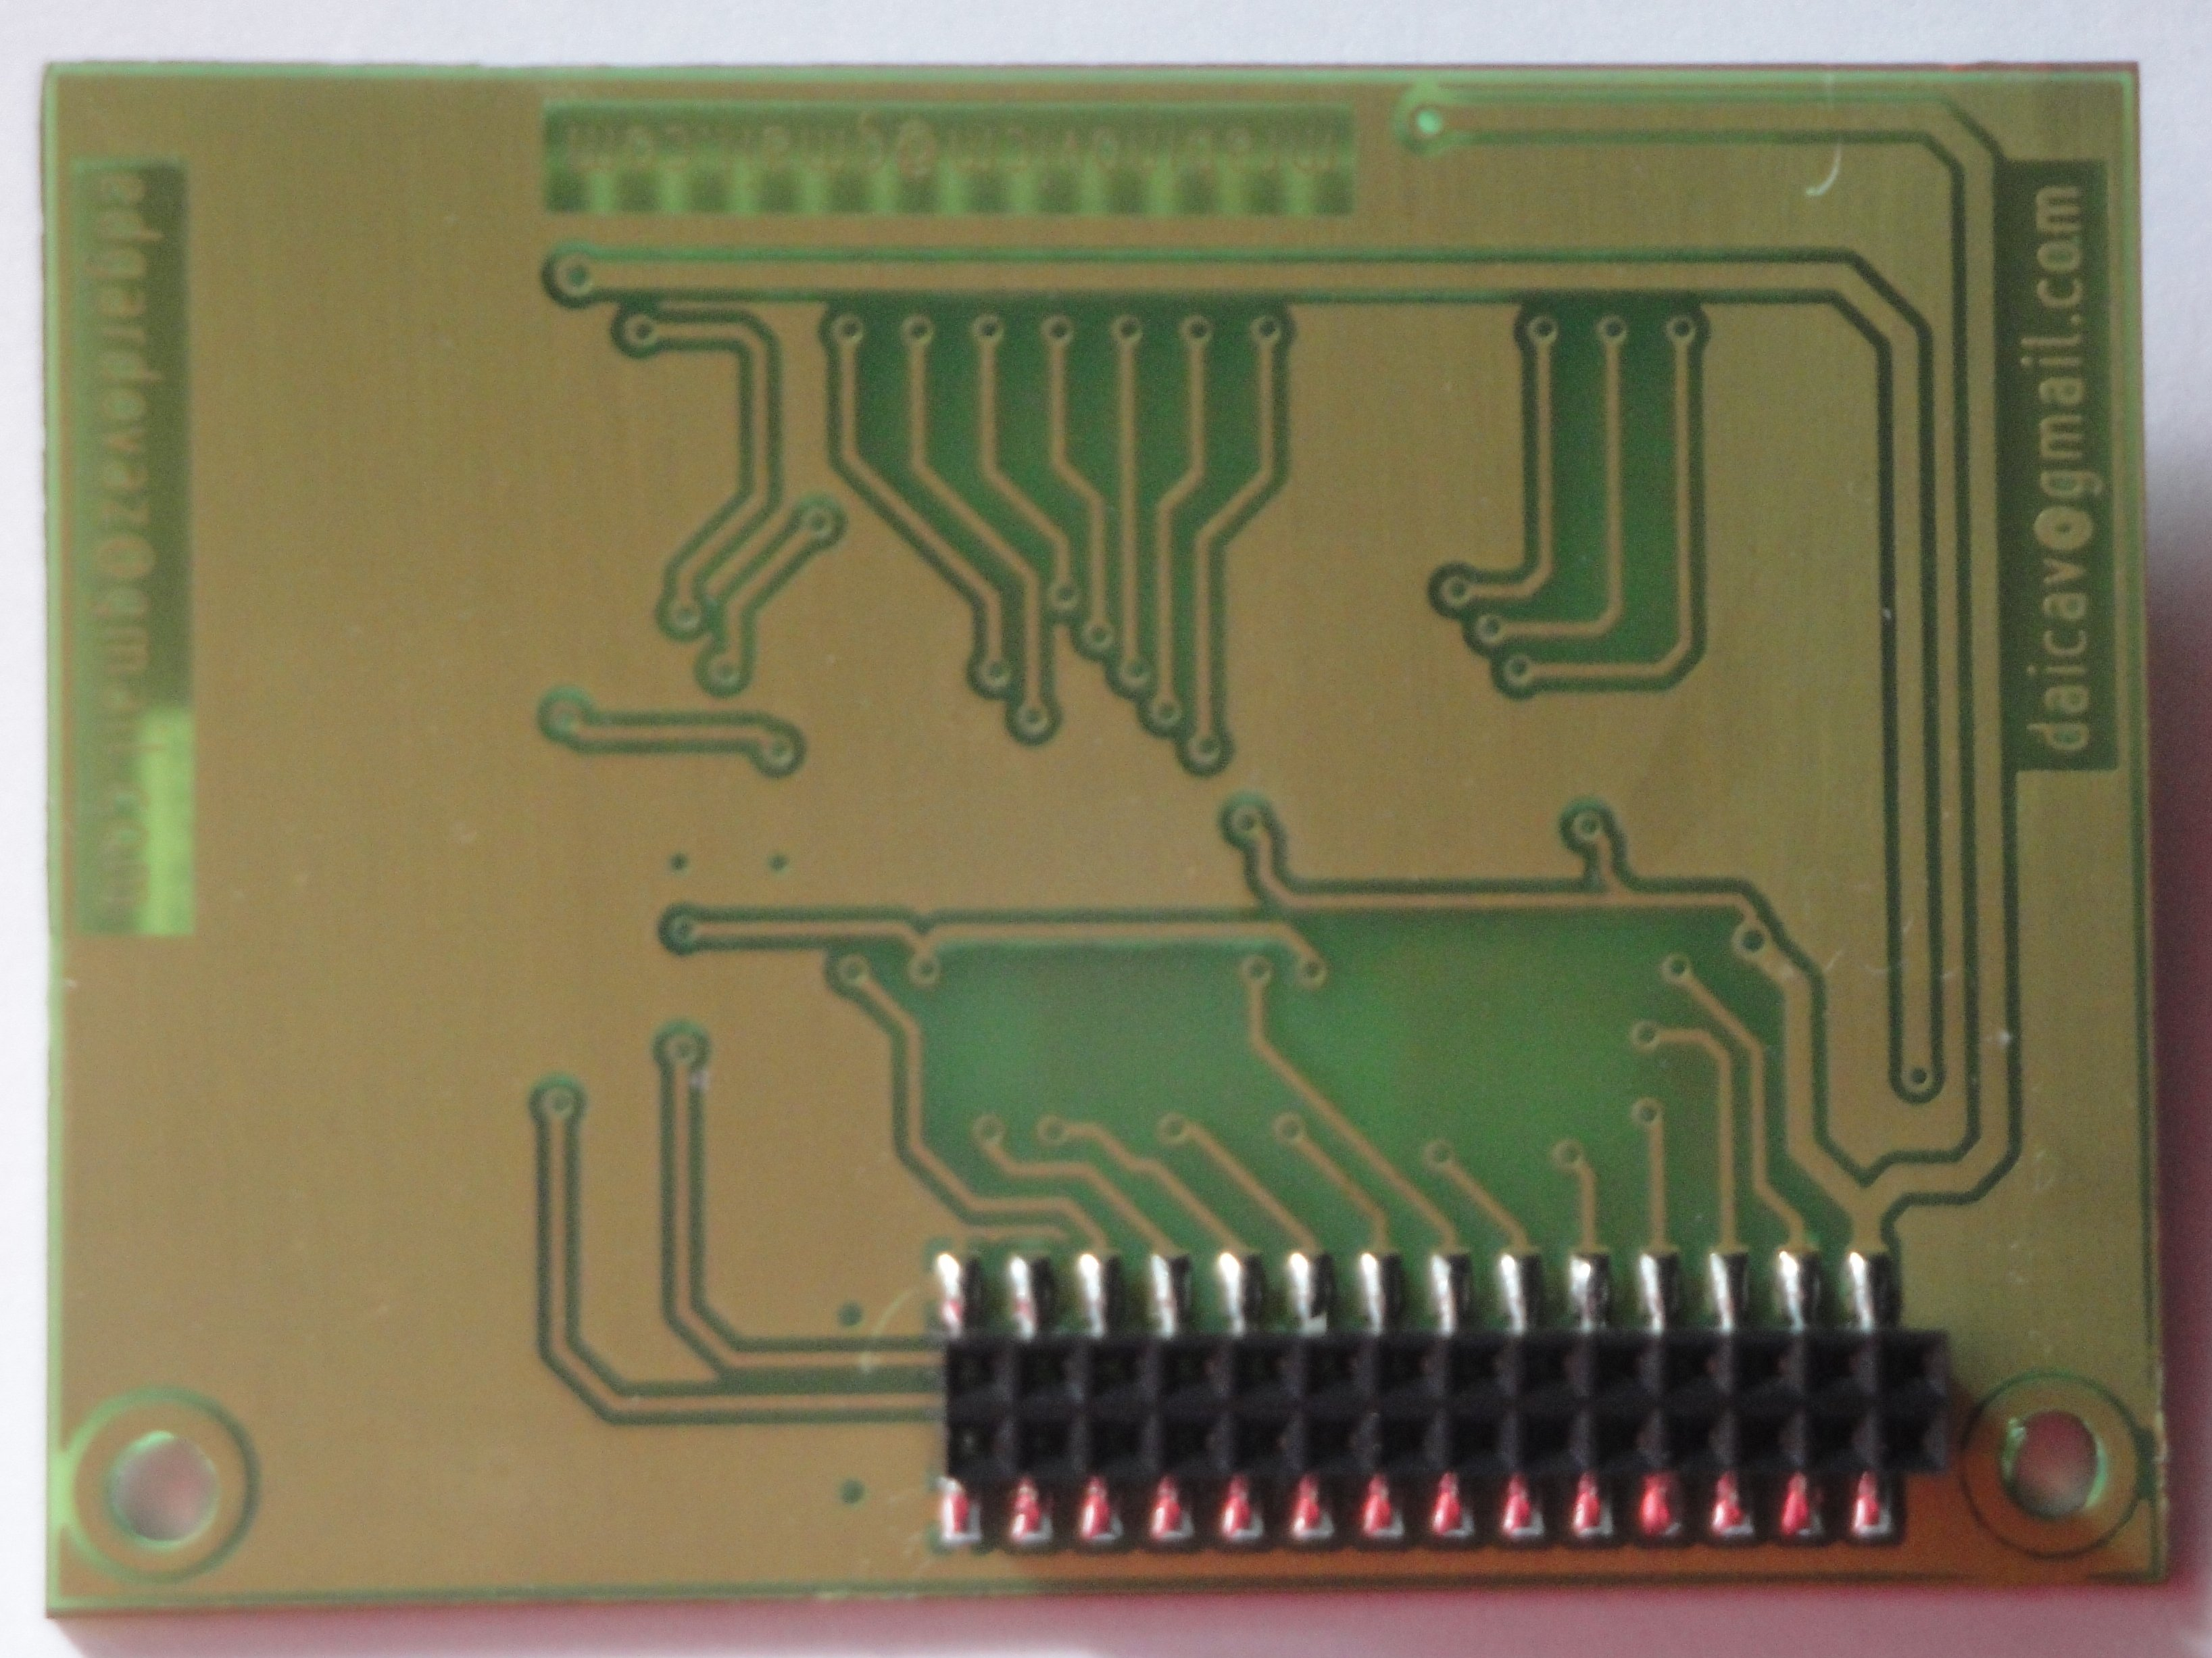
\includegraphics[scale=.08, angle=90]{Imagenes/VLT_b.jpg} }

  \caption{Vista anversa y reversa de VLT}\label{vltFB}
\end{figure}

\subsection{SCUI - Lector de tarjetas de contacto e Interfaz de Usuario}
El módulo SCUI puede dividirse en dos partes, una de ellas es un lector de tarjetas de contacto basadas en la norma ISO7816, y la otra es una simple interfaz para el usuario.
El lector de tarjetas de contacto (smart cards), está compuesto por un conversor full duplex a half duplex el cual se encuentra conectado a uno de los puertos UART de la SBC a través del módulo VLT, que se describió en el punto anterior. Este conversor permite la transmisión de datos directamente entre la tarjeta y la SBC, sin necesidad de intercalar un ASIC para el manejo de tarjetas del tipo ISO7816. Cuenta también con un oscilador para alimentar la entrada de reloj de las tarjetas. La entrada de control (OE) del oscilador operada desde la SBC permite poner la salida de reloj en tercer estado, cosa muy útil a la hora de cumplir con la secuencia de inicialización de las tarjetas descritas en el estándar. El lector permite operar con tarjetas clase A (alimentadas a 5 Volt) y clase B (alimentadas a 3,3 Volt) haciendo uso de un jumper que permite intercambiar la tensión de alimentación suministrada a la tarjeta. Se cuenta con un zócalo para insertar la tarjeta de contacto.
Por más detalles ver esquemático en la figura \ref{Fig:SAM}.

Por otra parte, la intefaz de usuario está compuesta por tres leds (verde, amarillo y rojo), buzzer y un display LCD16x2 donde son desplegados los mensajes que indican al usuario la operación que se efectúa sobre su tarjeta Mifare.
Por más detalles ver esquemático en la figura \ref{Fig:UI}.

El último elemento a describir aquí es un conector receptáculo 5x2 (100mils) en el que se conecta el módulo lector/escritor RFID que opera con las tarjetas RFID Mifare.
Por más detalles ver esquemático en la figura \ref{Fig:SCUI}.

\begin{figure}[H]
  \centering
  \subfigure[Vista anversa de SCUI]{\label{scuiF}
  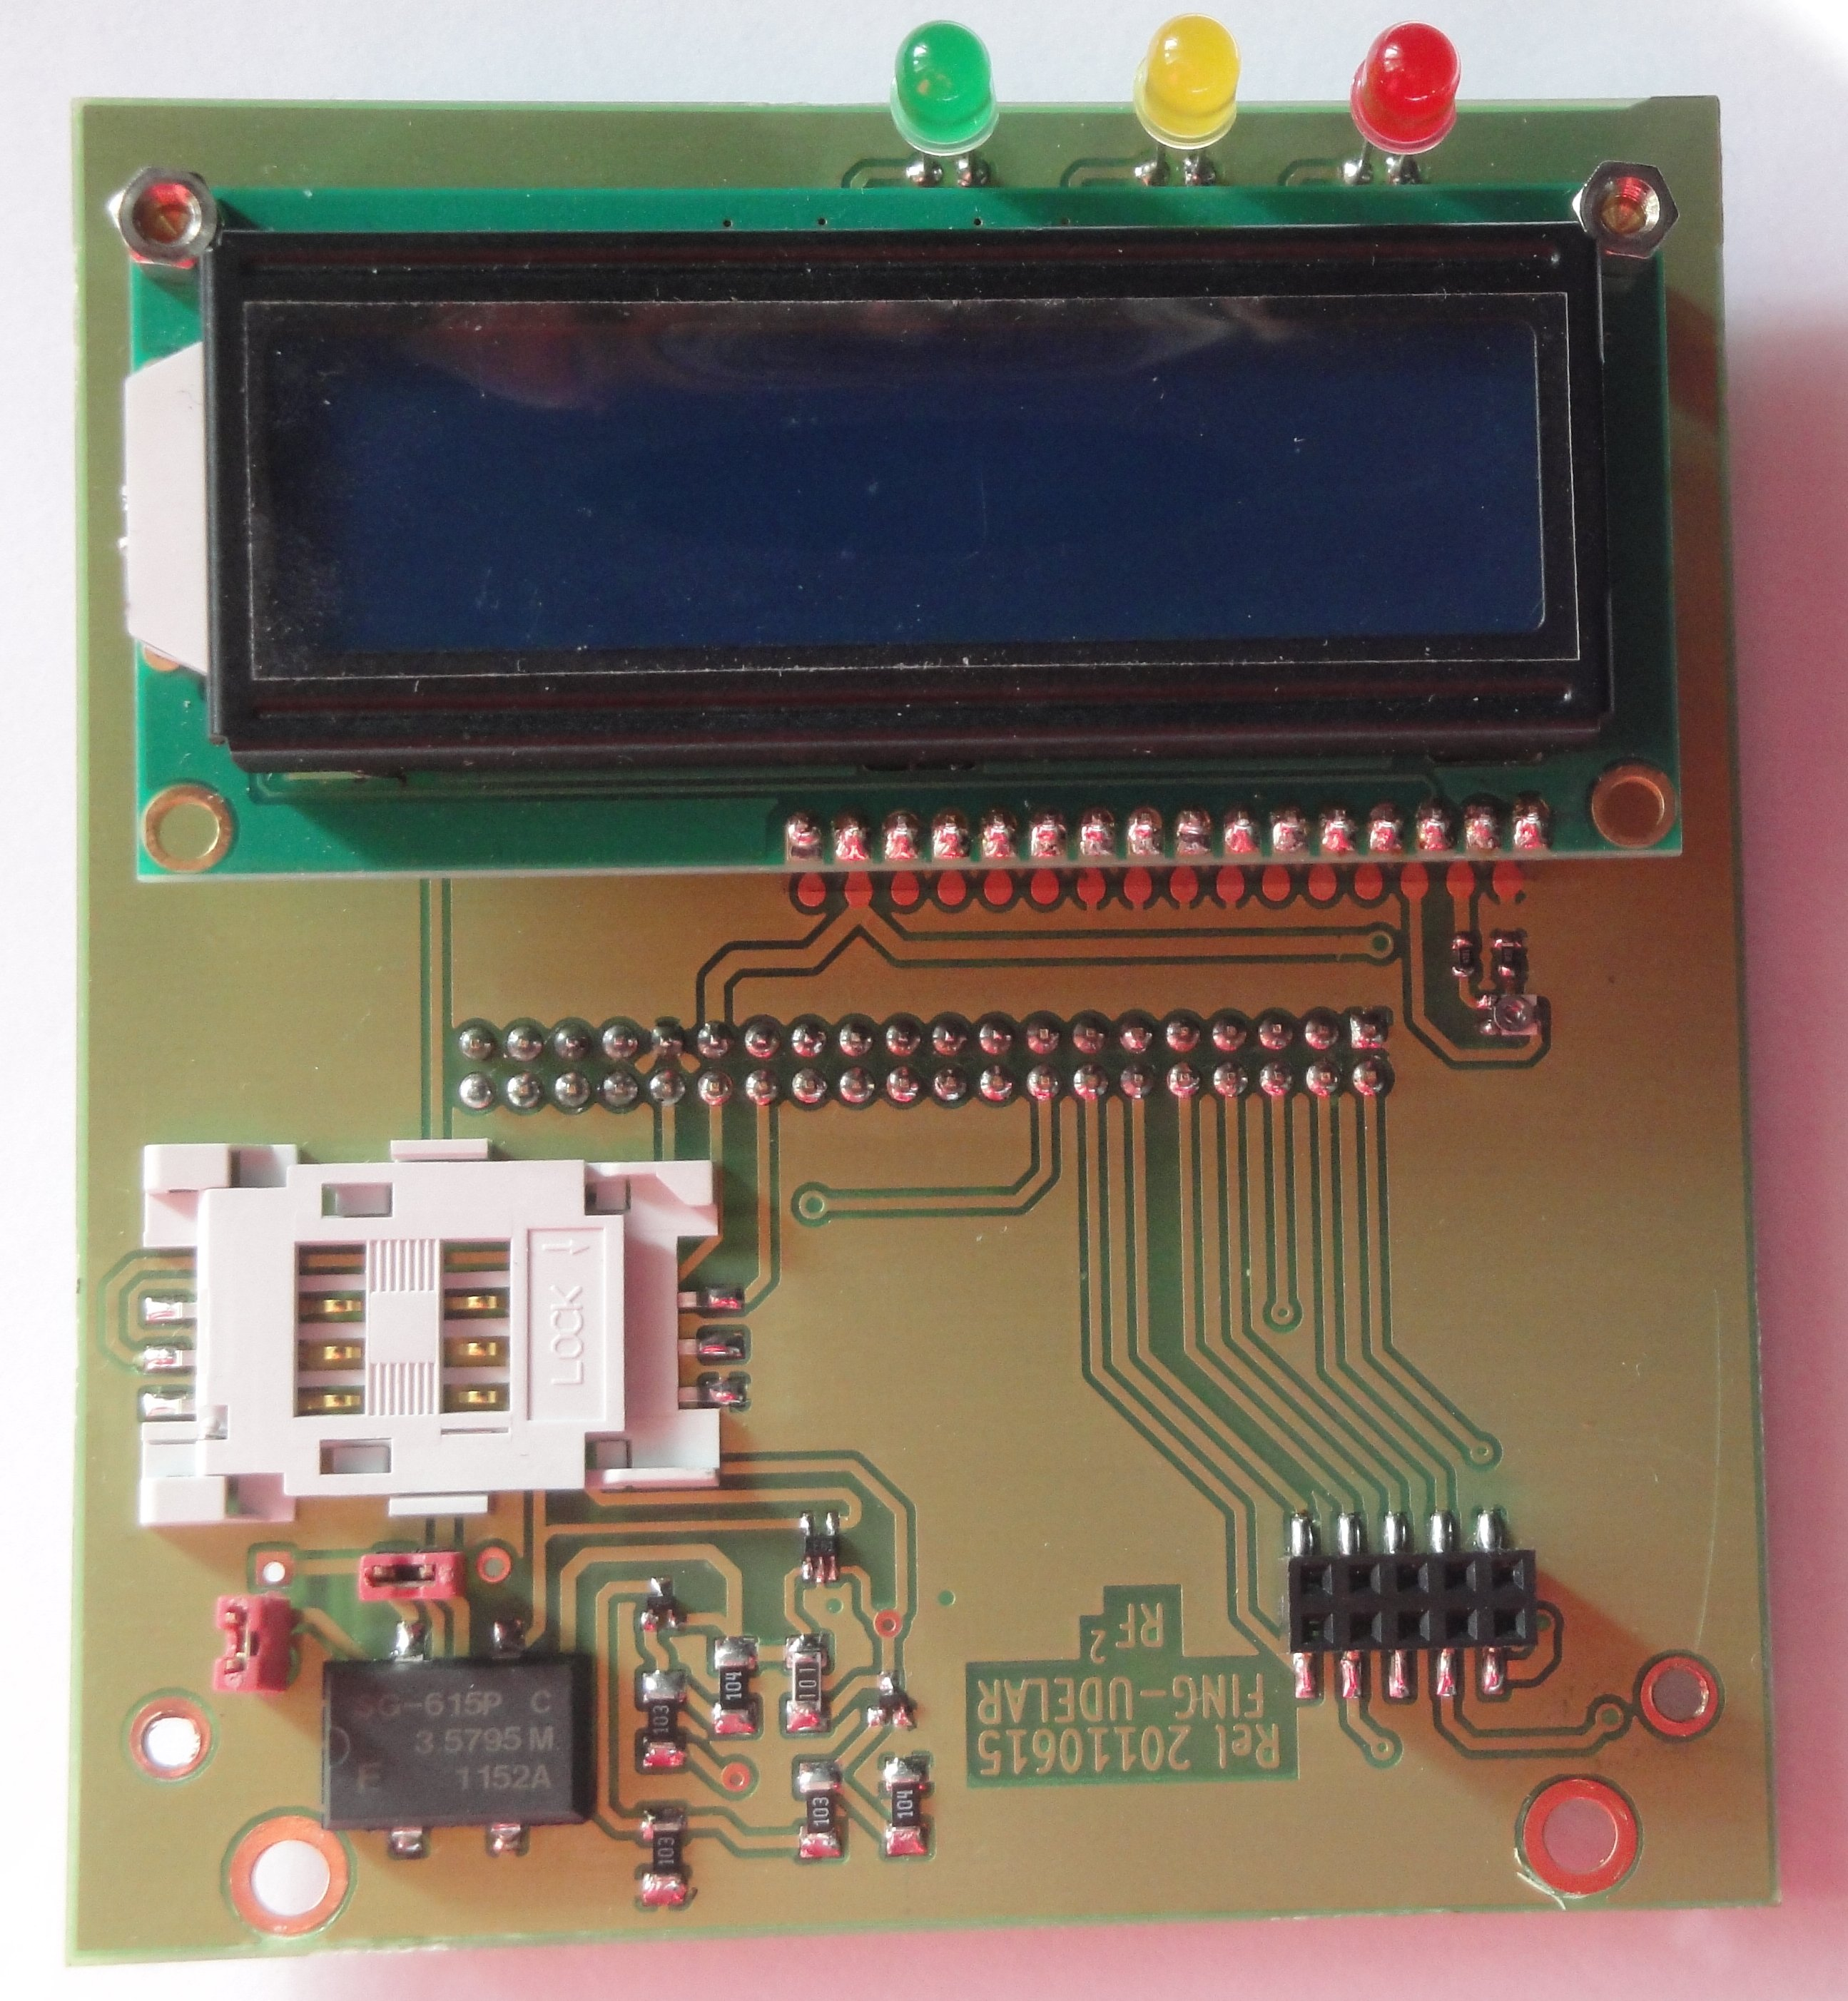
\includegraphics[scale=.07]{Imagenes/SCUI_f.jpg} } 
  \subfigure[Vista reversa de SCUI]{\label{scuiB} 
  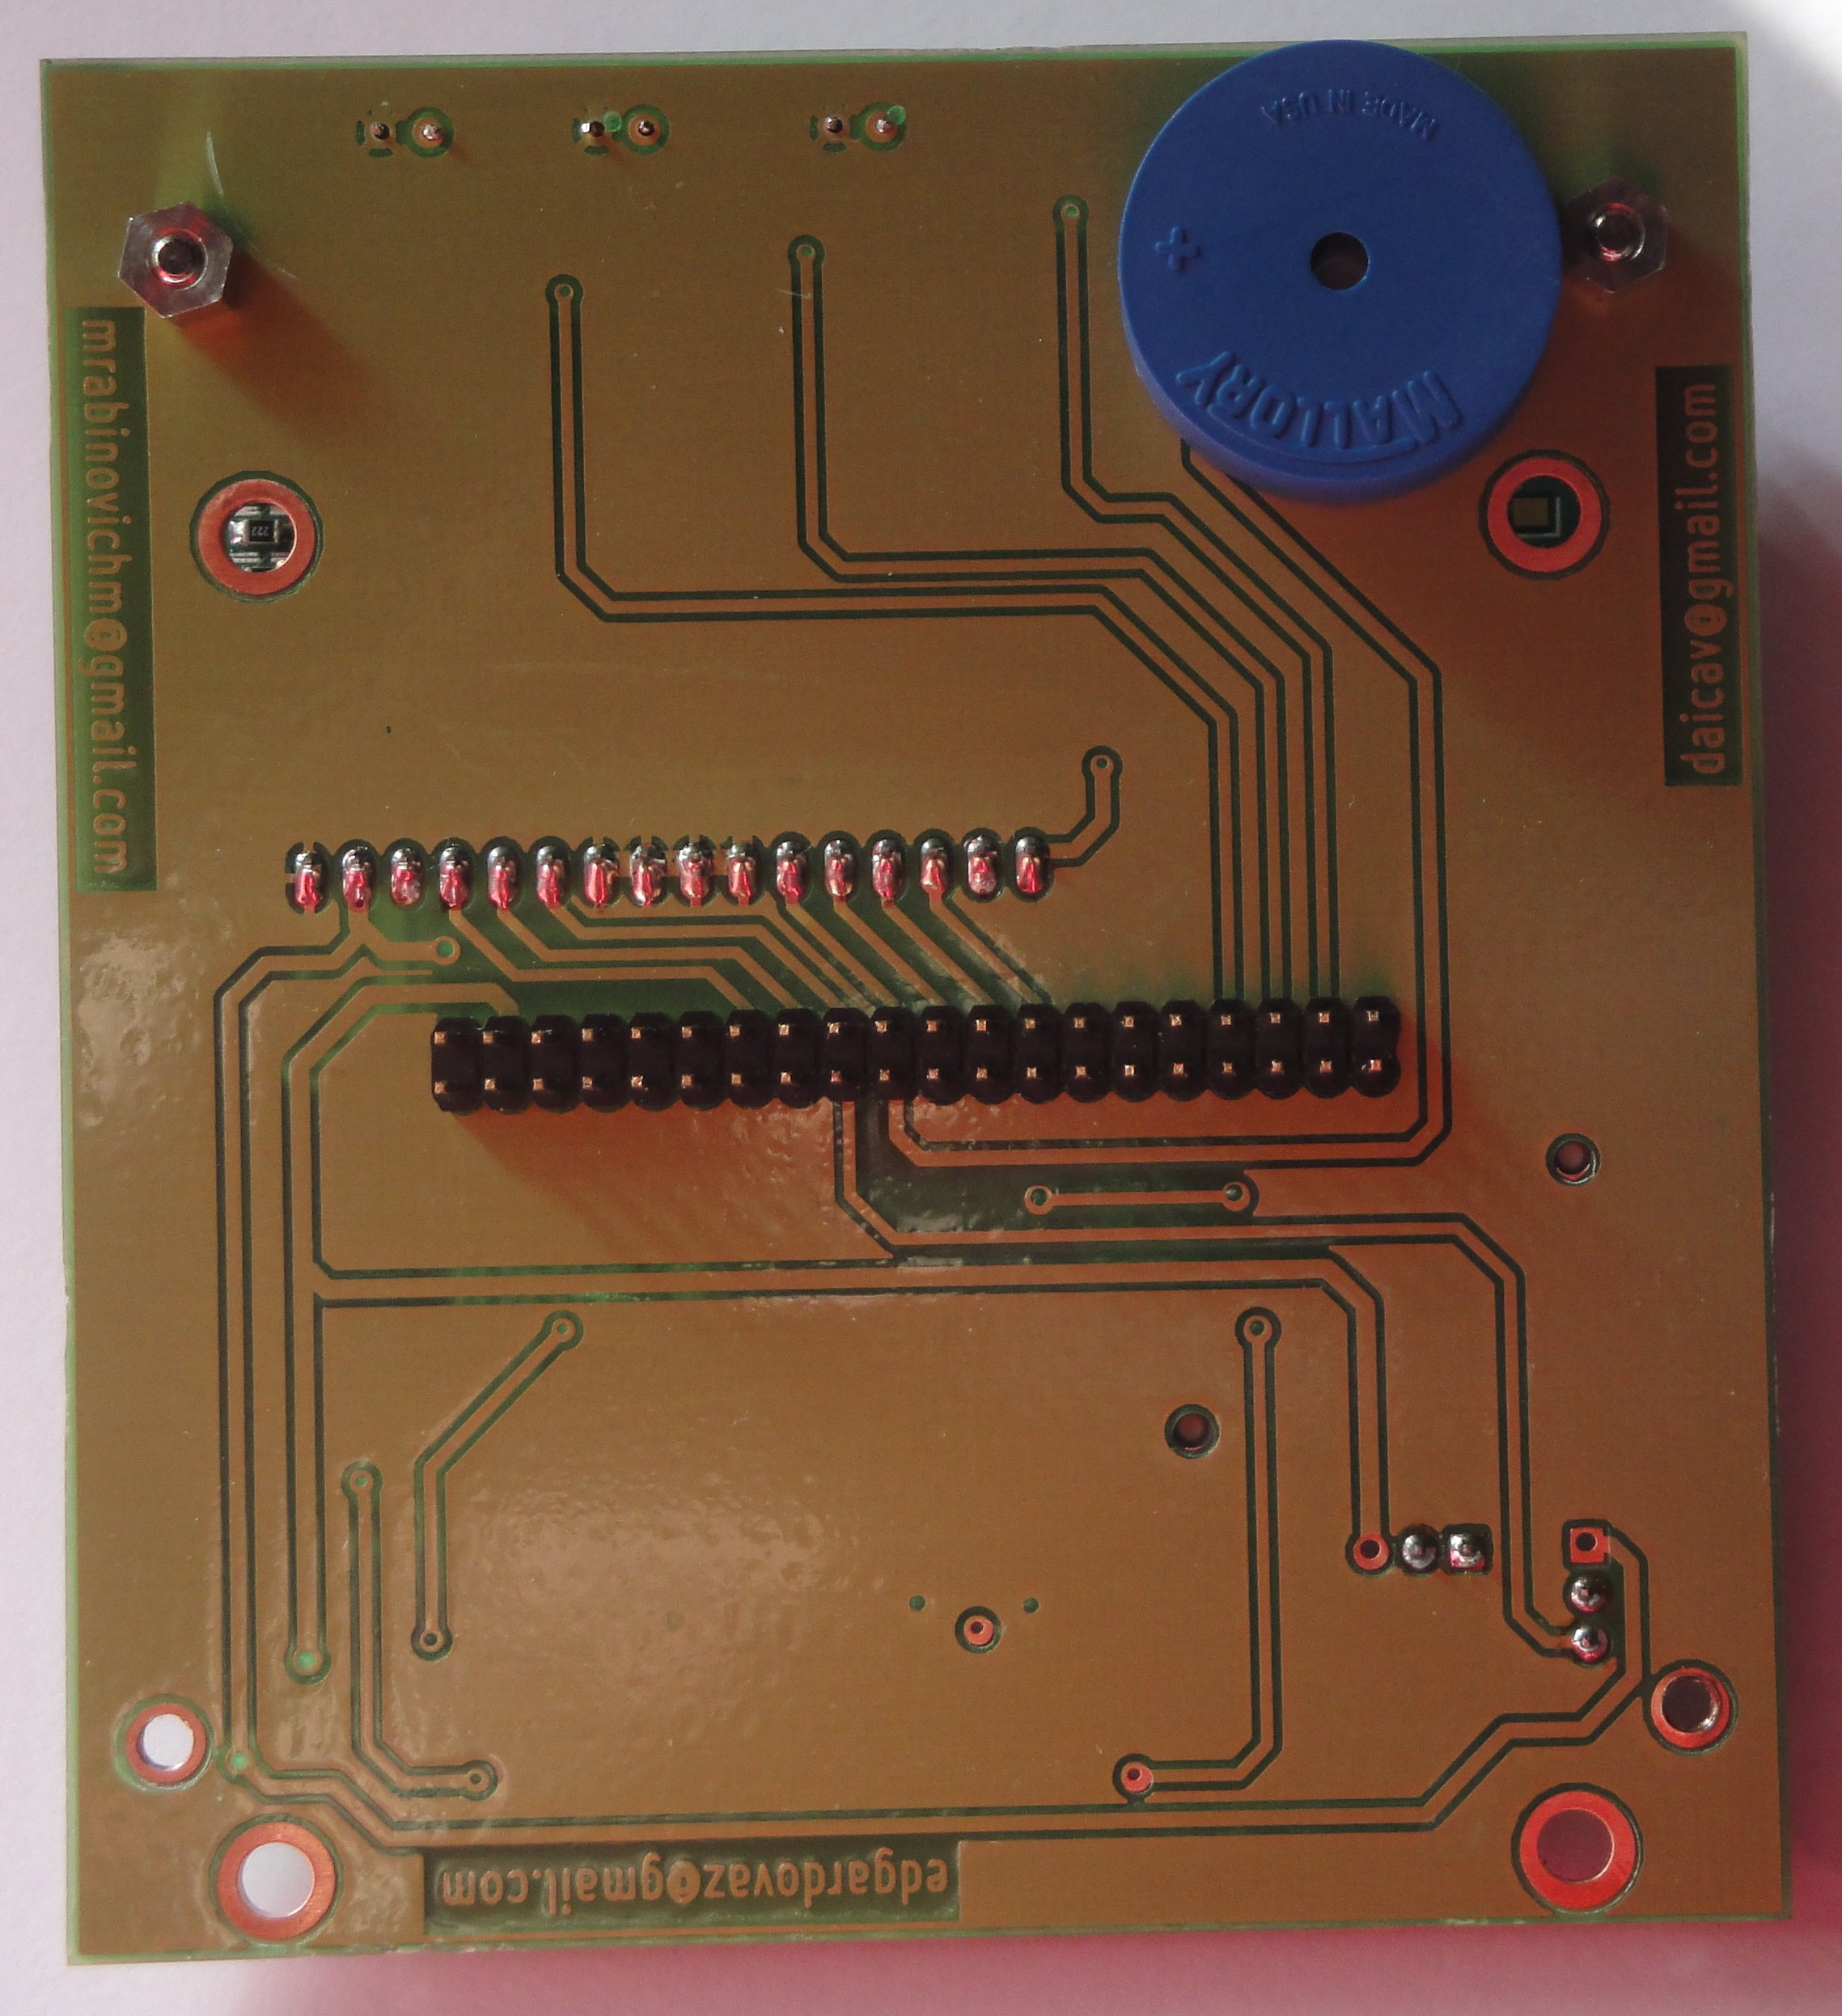
\includegraphics[scale=.08]{Imagenes/SCUI_b.jpg} }

  \caption{Vista anversa y reversa de SCUI}\label{scuiFB}
\end{figure}

\newpage
\subsection{Lector/Escritor RFID}
Este módulo es el encargado de la comunicación con las tarjetas RFID que cumplen con la norma ISO14443. Consta básicamente de cuatro secciones entre las que se encuentran: el integrado CL RC632; el filtro EMC, el circuito de adaptación de impedancia (matching); y el inductor de la antena. 
El ASIC CL RC632 permite, por un lado la comunicación digital con un microprocesador a través de su puerto de datos y por el otro lado la transmisión de datos hacia la antena que emitirá la señal RF para la comunicación con las tarjetas ISO14443.
Por más detalles ver esquemático en la figura \ref{Fig:RFID}.

Lo que se llama propiamente antena RF está conformada por el circuito de adaptación de impedancia (matching) y por el inductor ubicado en el circuito impreso, que propaga el campo magnético para lograr el acoplamiento necesario entre lector y tarjeta, de aquí la sigla PCD (Proximity Coupling Device).
Por más detalles ver esquemático en la figura \ref{Fig:RFID2}.

Los principios básicos de funcionamiento de la antena se detallan en el apéndice \ref{anx_antena}.

\begin{figure}[H]
  \centering
  \subfigure[Vista anversa del lector/escritor RFID]{\label{scuiF}
  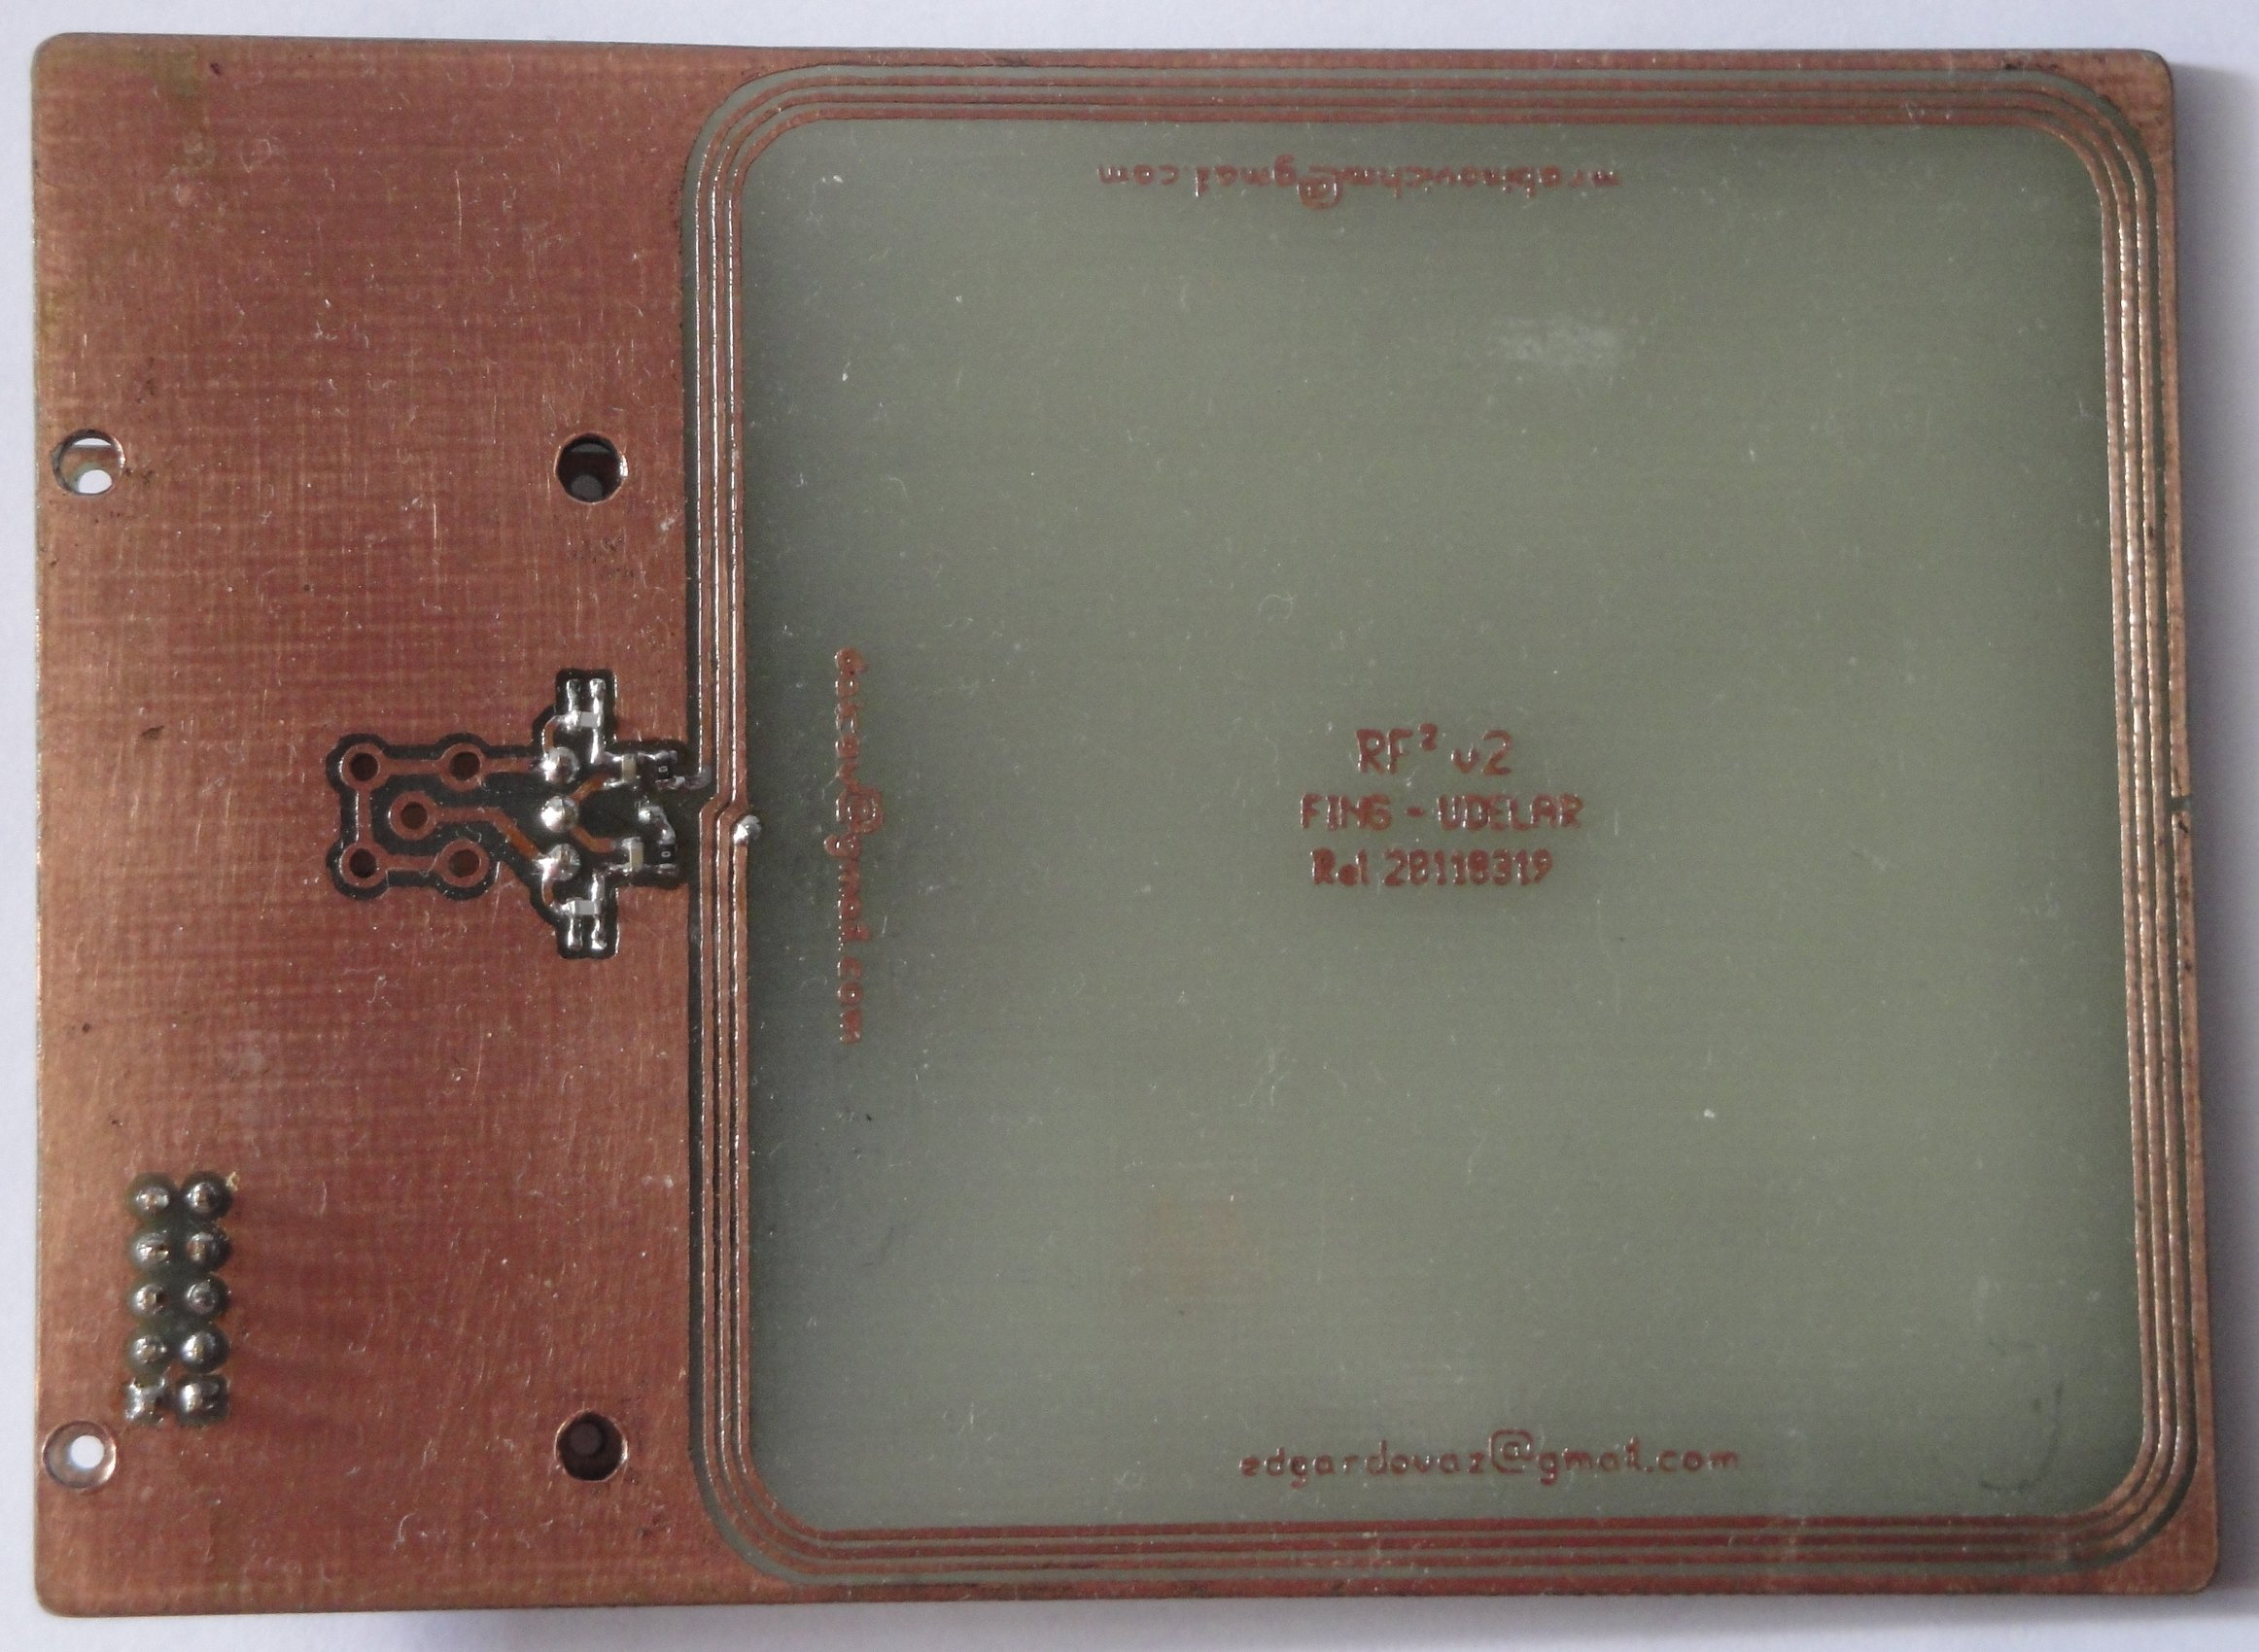
\includegraphics[scale=.08]{Imagenes/ant_f.jpg} } 
  \subfigure[Vista reversa del lector/escritor RFID]{\label{scuiB} 
  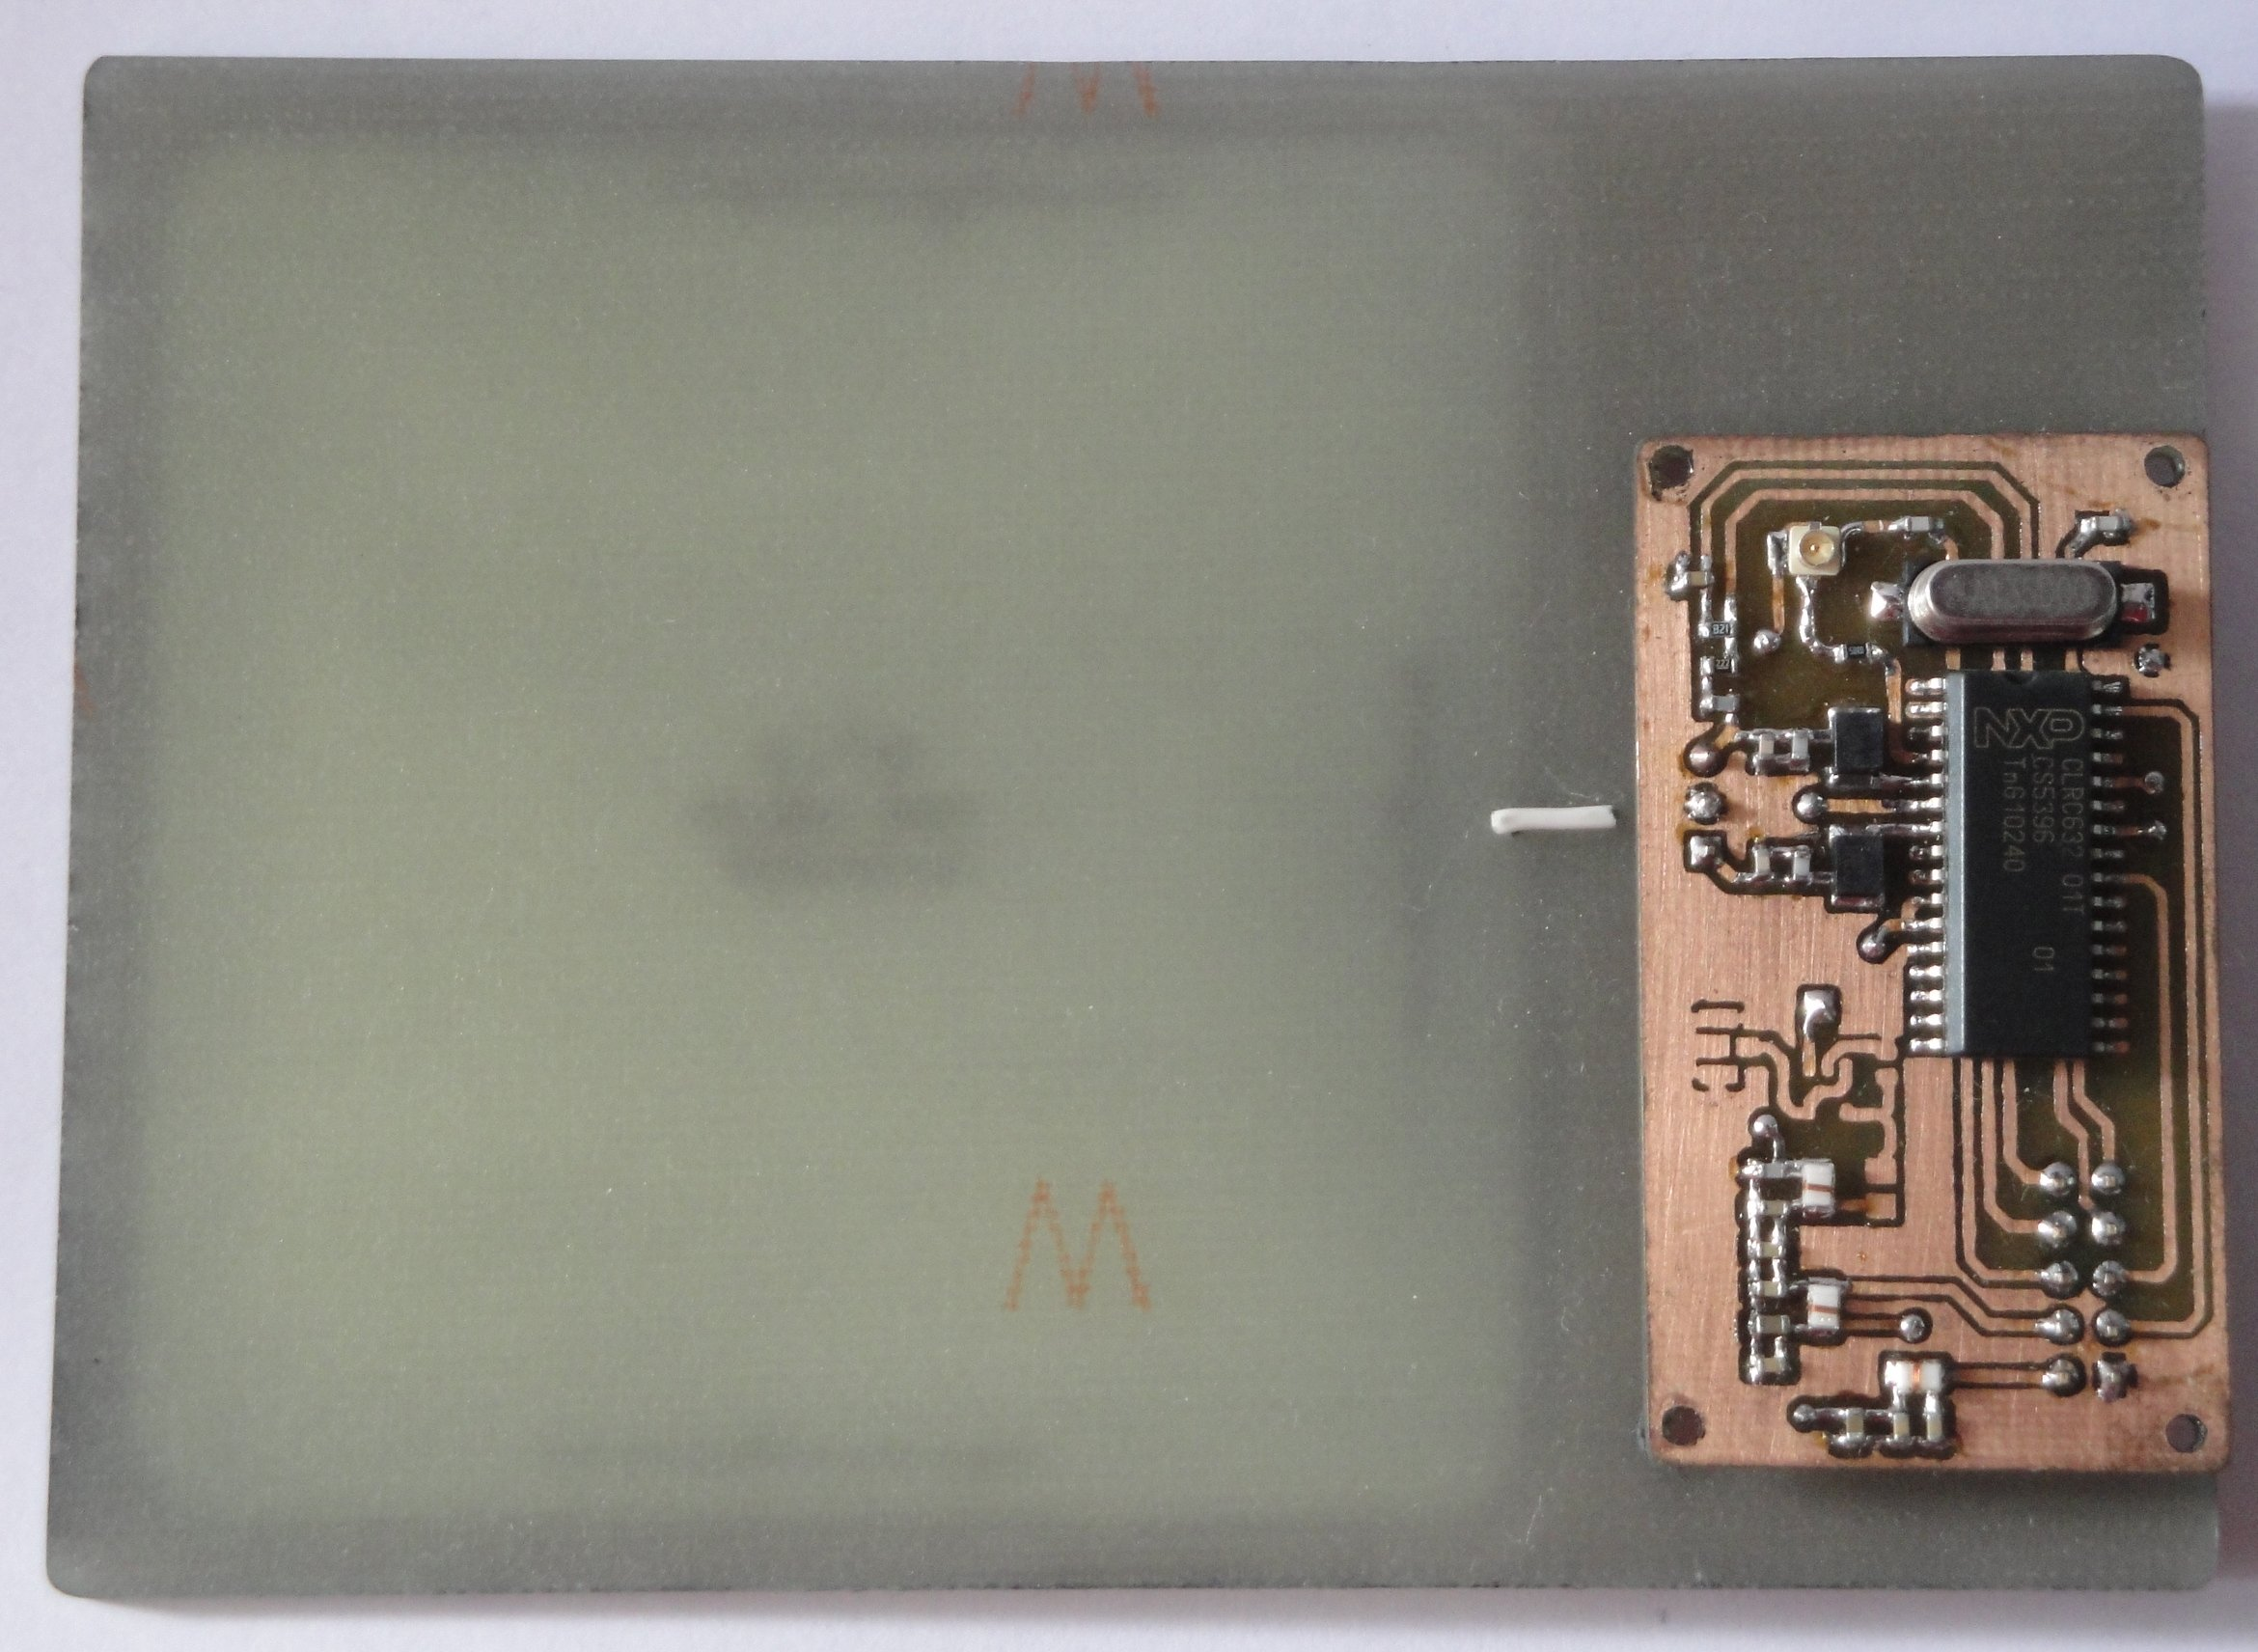
\includegraphics[scale=.08]{Imagenes/ant_b.jpg} }

  \caption{Vista anversa y reversa del lector/escritor RFID}\label{l/eRFID}
\end{figure}

\bigskip
Por detalles de esquemáticos y listas de componentes referirse al apéndice \ref{docHW}.

\newpage
\section{Funcionamiento de m\'odulos}

\subsection{SBC}
La SBC está formada por un SOC y memoria suficiente para ejecutar un sistema operativo GNU/Linux orientado a desarrollar sistemas embebidos. Sobre el sistema operativo se instalan los módulos y bibliotecas necesarias para hacer uso del hardware que contiene la SBC. En la aplicación se utilizará uno de sus puertos SPI para la comunicación con el lector/escritor de tarjetas RF, un puerto UART para la comunicación de datos con el lector de tarjetas de contacto y varias salidas GPIO para el control de la interfaz de usuario.

\subsection{VLT - Conversor de Voltajes}
El corazón de esta placa son los integrados TXB0108 \cite{HD_VLT} (ver hoja de datos en el apéndice \ref{HD}) que permiten la interconexión de dispositivos que operan en distintos niveles de tensión. Básicamente el integrado está constituído por dos puertos, puerto A y puerto B cada uno de 8 bits. El puerto A opera con la tensión de 1,8 Volt que permite ser conectado a la Beagleboard, el puerto B opera con la tensión de 3,3 Volt cuando se encuentra conectado al CL RC632, y de 5 Volt para los restantes periféricos.
Cada I/O de un puerto es sensible a los flancos de subida o bajada, trasladando estos cambios a la I/O correspondiente del puerto opuesto. 
Este integrado posee también una entrada de control para poner los puertos en estado de alta impedancia.
Una ventaja es que no poseen entrada de control de dirección de flujo de datos, de modo que se ahorran pines de control que no se tienen disponibles en la Beagleboard.
En la figura \ref{Fig:Celda_TXB0108} se puede observar como están constituídas cada una de las entradas/salidas del integrado.
Otra pieza que compone esta placa es el regulador de tensión LDO implementado a partir del integrado LM1117 \cite{LDO} (ver hoja de datos en el apéndice \ref{HD}), éste se utiliza para convertir la entrada de tensión de 5 Volt en una salida de tensión de 3,3 Volt y así poder alimentar el periférico correspondiente.

Por más detalles ver esquemático en la figura \ref{Fig:VLT}.

\bigskip
\bigskip
\begin{figure}[H]
\centering
  \begin{center}
  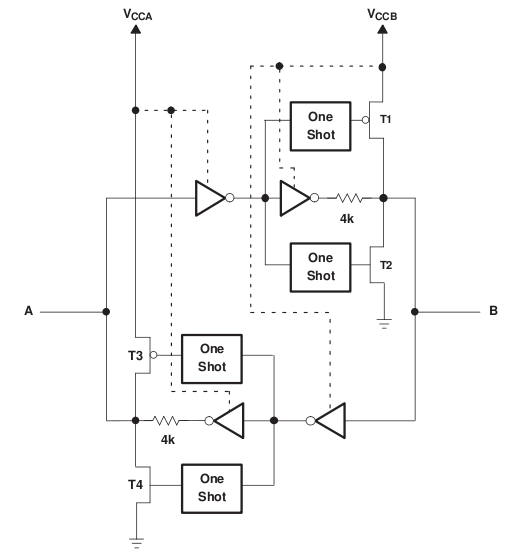
\includegraphics[scale=.3]{Imagenes/TXB0108.png} 
  \end{center}
  \caption{Arquitectura de una celda I/O del TXB0108}\label{Fig:Celda_TXB0108} 
\end{figure}


\subsection{SCUI - Lector de tarjetas de contacto e Interfaz de Usuario}

\leftline{\bf{Lector de tarjetas de contacto ISO7816}}

Es un lector muy simple de implementar, su construcción se basa en un conversor full a half duplex construido a partir de un circuito transistorizado trabajando en zona de corte y saturación. Los transistores empleados son el NPN 2N3904 (ver hoja de datos en el apéndice \ref{HD}) y el PNP 2N3906 (ver hoja de datos en el apéndice \ref{HD}) los cuales fueron seleccionados en base a su rápida característica de conmutación que es del orden de algunas decenas de nanosegundos. Dada la característica del circuito, es posible recibir el eco de la transmisión de datos generados por la SBC. 
Un elemento fundamental que compone el circuito del lector es el oscilador de frecuencia 3,579545 MHz, este valor no es antojadizo sino que permite generar la base de tiempo adecuada para la transmisión de datos entre la tarjeta y la SBC. Otras frecuencias de reloj fueron empleadas, como ser 4 MHz y 5 MHz, con resultados inciertos en la recepción de los datos, aún cuando sería posible usar estos valores según la referencia \cite{SCHb} para los parámetros obtenidos desde el ATR de la tarjeta. 
El circuito cuenta también con protección de descarga ESDA6V1W5 (ver hoja de datos en el apéndice \ref{HD}) para los contactos de la smart card.

Por más detalles ver esquemático en la figura \ref{Fig:SAM}.

\newpage
\leftline{\bf{Interfaz de usuario}}

El elemento a destacar es un display LCD16x2 que basa su funcionamiento en el controlador Hitachi HD44780 \cite{dpy} (ver hoja de datos en el apéndice \ref{HD}). La transferencia de datos hacia el display se hace a través de un puerto con 4/8 bits de datos y 3 bits de control. Debido a que no se cuenta con la cantidad de pines disponibles en la Beagleboard para operar en el modo de 8 bits, se empleó en su lugar el modo 4 bits del display. El bit de control RS indica si el byte a enviar por el puerto de datos es una palabra de control o un caracter ASCII a ser almacenado en la memoria interna del display. El bit R/W por su parte indica si se efectuará una lectura o una escritura de la memoria interna del display. Por último en el bit E se indica mediante flanco de bajada que se ejecute la operación indicada con los anteriores dos bits de control, previo a este flanco las señales en el puerto de datos deben permanecer fijas.
El display cuenta también con una entrada para calibrar el contraste del LCD, la calibración se realiza a partir de un divisor resistivo implementado con resistencias y un preset.
El backlight del display es accionado desde uno de los pines de la SBC a partir de un circuito transistorizado que opera en zona de corte/saturación.
Los restantes elementos que componen la interfaz de usuario son leds y buzzer que son accionados directamente desde los pines del puerto de expansión de la SBC.

Por más detalles ver esquemático en la figura \ref{Fig:UI}.

\subsection{Lector/Escritor RFID}
En el corazón del lector/escritor de tarjetas RFID, se encuentra el chip CL RC632 que forma parte de una familia de integrados empleados para la comunicación con tarjetas sin contacto, pertenecientes a la norma ISO14443 las cuales operan a la frecuencia 13,56 MHz.
El CL RC632 soporta todas las capas del esquema de comunicación que se establecen en la mencionada norma, incluyendo el algoritmo de seguridad (CRYPTO1) para encriptar el canal de comunicación con las tarjetas Mifare Classic. En lo que sigue se describen algunas de las características principales del integrado.

Por más detalles ver esquemático en la figura \ref{Fig:RFID}.

\newpage
\leftline{\bf{Interfaz}}

Los comandos, bits de configuración y las banderas se acceden a través de la interfaz con un microprocesador. El puerto elegido para la comunicación desde la SBC es el SPI, aunque es posible la comunicación a través de su puerto paralelo. 

\bigskip
\leftline{\bf{Registros}}\label{Registros}

La configuración del chip se lleva a cabo a partir de un mapa de registros de control que se encuentra dividido en 8 páginas con 8 registros cada una. La manera de alcanzar estos registros es mediante el intercambio de página, mecanismo que puede ser deshabilitado mediante escritura de un “1” en el bit 7 del registro 0 en la página 0, logrando direccionamiento plano. La función de cada uno de sus registros puede ser observada en la hoja de datos del integrado \cite{RC632} (ver apéndice \ref{HD}).

\bigskip
\leftline{\bf{Memoria EEPROM}}

La memoria está dividida en 32 bloques con 16 bytes cada uno.
El contenido de memoria EEPROM en los bloques 1 y 2 (dirección 10hex a 2Fhex) se utilizan para configurar los registros del CL RC632 durante la fase de inicialización, de forma automática.
La configuración por defecto soporta la comunicación Mifare ISO 14443 A, aunque los usuarios pueden especificar la inicialización para I-Code1, ISO 15693 o ISO 14443 B, mediante los bloques de memoria 3 al 7.
Se reservan 384 bytes para almacenar las claves CRYPTO1 que son usadas para la autenticación con las tarjetas. El formato de una de estas claves puede verse en \cite{RC632} (ver apéndice \ref{HD}) y tiene una longitud de 12 bytes, por tanto es posible almacenar en memoria las 32 claves que posee una tarjeta.

\bigskip
\leftline{\bf{Buffer FIFO}}

El integrado contiente un buffer FIFO de 64 bytes para flujo de datos con un microprocesador.
La entrada y salida del buffer de datos está conectado con el registro FIFOData. Escribir en este registro almacena un byte en el buffer e incrementa el puntero de escritura del buffer. La lectura de este registro muestra el contenido del buffer e incrementa el puntero de lectura. La distancia entre el puntero de escritura y lectura se puede obtener mediante la lectura del registro FIFOLength, indicando así la cantidad de bytes que se llevan almacenados. Es posible observar y controlar el estado del buffer mediante varios registros, para evitar que se produzcan errores de comuncicación con el microprocesador.

\bigskip
\leftline{\bf{Interrupciones}}

El CL RC632 indica ciertos eventos estableciendo el bit IRQ en el registro \\
PrimaryStatus, y además, por la activación del pin IRQ. La señal en el pin IRQ se puede utilizar para interrumpir un micrprocesador. 
Las posibles fuentes de interrupción son: 

\begin{itemize}

\item Timer, a través de su bandera TimerIRq 
\item Transmisor, coprocesador CRC y memoria E2PROM, a través de su bandera TxIRq 
\item Receptor, a través de su bandera RxIRq 
\item Registro de comando, a través de su bandera IdleIRq 
\item Buffer FIFO, a través de sus banderas HiAlertIRq y LoAlertIRq 

\end{itemize}

El CL RC632 informa al microprocesador sobre el origen de una interrupción mediante el establecimiento del bit adecuado en el registro InterruptRq. La relevancia de cada bit de petición de interrupción como fuente de una interrupción puede ser enmascarada con el bit de habilitación de interrupciones en el registro InterruptEn. 
Si alguna bandera de solicitud de interrupción se establece en 1 (una solicitud de interrupción está pendiente) y la correspondiente bandera de habilitación de interrupción está en "1", la bandera de estado IRq en el registro PrimaryStatus se establece en 1. 
Por otra parte diferentes fuentes de interrupción pueden estar activas al mismo tiempo. Por lo tanto, se hace un OR con todos los bits de solicitud de interrupción, el resultado se envía a la bandera IRq y se conecta al pin IRQ. 
Los bits de petición de interrupciones están seteados de forma automática por las máquinas de estado internas del CL RC632. Adicionalmente, el microprocesador tiene acceso para setearlos o borrarlos. 
Una implementación especial de los registros InterruptRQ y InterruptEn permiten el cambio de un único bit de estado sin tocar el resto. 

\bigskip
Configuración del Pin IRQ:
El nivel lógico de la bandera de estado IRq es visible por el pin IRQ. Además, la señal en el pin puede ser controlada por los siguientes bits del registro IRQPinConfig 
\begin{itemize}
\item IRQInv: Si este bit es 0, la señal en el pin IRQ es igual al nivel lógico del bit IRq. 
Si es 1, la señal en el pin IRQ está invertida con respecto al bit IRq. 
\item IRQPushPull:  Si este bit es 1, el pin IRQ tiene características de una salida estándar 				   CMOS, de otra manera la salida es open drain y un resistor externo es necesario para alcanzar un nivel alto en este pin. 
\end{itemize}

Para poder hacer uso de lo descrito anteriormente se previó y reservó una entrada en el conector de expansión de la Beagleboard (ver figura \ref{Fig:VLT}), sin embargo el software empleado no hace uso del mecanismo de interrupciones sino que opera mediante polling.

\bigskip
\leftline{\bf{Transmisor, pines Tx1 y Tx2}}

La señal en Tx1 y Tx2 es la portadora, centrada en 13,56 MHz, modulada ASK 100\% con los datos a transmitir. Estos pines son conectados directamente a la antena para propagar la señal RF hacia las tarjetas RFID. La distancia de operación alcanzada es de hasta 10cm de longitud, dependiendo de la geometría de la antena, así como también adaptación de impedancia lograda, entre otros (ver \cite{MRICF} y \cite{RFIDPA} incluídas en el apéndice \ref{HD}).
Algunos registros del integrado permiten la configuración del transmisor, posibilitando entre otras cosas apagar la señal portadora en caso de ser necesario.

\bigskip
\leftline{\bf{Conjunto de comandos}}

El CL RC632 opera como una máquina de estado capaz de interpretar y ejecutar un conjunto de comandos pre establecidos. La ejecución de uno de ellos es posible escribiendo su código correspondiente en el “Registro de Comandos”, si fuera necesario el pasaje de parámetros, éstos se colocarán en el buffer FIFO mencionado antes. 
Una lista detallada de comandos junto con los parámetros necesarios es mostrada en la hoja de datos (ver apéndice \ref{HD}), entre ellos se pueden destacar los siguientes: Authent, Transceive, LoadKey.

\bigskip
\leftline{\bf{Antena RF}}

En lo que sigue se describen algunas de las partes que integran la antena RF que se conecta directamente a los pines Tx1 y Tx2 del integrado descrito antes.

\bigskip
\leftline{\bf{Filtro EMC}}

La frecuencia de la portadora de la señal transmitida se centra en 13,56 MHz, sin embargo se generan también armónicos de mayor frecuencia. Para cumplir con la regulación internacional EMC es que se agrega este filtro pasa bajos, cuya frecuencia de corte debe ubicarse en 14,4 MHz, o sea 13,56 MHz más 847,5 KHz para permitir el ancho de banda necesario que logre el baud rate requerido en la transmisión de los bits. 
En síntesis el filtro ayuda a mejorar la relación señal a ruido para la señal recibida y decrementa el sobretiro en los pulsos transmitidos mejorando la calidad de la señal transmitida.
Los valores propuestos para los componentes de este filtro se encuentran en las notas de aplicación \cite{MRICF}.

\bigskip
\leftline{\bf{Matching}}

Por su parte, el circuito de adaptación de impedancia permite que la antena resuene a la frecuencia deseada, en este caso 13,56 MHz. Los valores de los elementos que conforman este circuito deben ser estimados y sintonizados a partir del diseño del inductor de la antena.
El factor de calidad total de la antena debe ser tenido en cuenta para cumplir con los requerimientos establecidos en la norma ISO14443. 
El mecanismo para el cálculo de los elementos que foman este circuito se detallan en las notas de aplicación \cite{MRICF}, referirse al apéndice \ref{capresonan}. 

\bigskip
\leftline{\bf{Inductor}}

El inductor de la antena es quien propaga el campo magnético para la transmisión de datos hacia las tarjetas. El diseño de la antena comienza a partir de este elemento.
El cálculo detallado del valor del inductor se encuentra en las notas de aplicación \cite{ACD}, aunque su costo y tiempo en la práctica son considerables; una estimación del valor de la inductancia puede verse en el apéndice \ref{anx_antena}, en el que se deben tener en cuenta los siguientes elementos: geometría de la antena, ancho y espesor del conductor del PCB, longitud de una espira, número de vueltas, etc. En este caso el tipo de PCB utilizado para la fabricación del inductor es FR-4.

\bigskip
\leftline{\bf{Receptor}} 

El circuito receptor de la antena se encuentra bien detallado en las notas de aplicación \cite{MRICF} y no fue necesario efectuar ningún cambio para lograr buenos resultados en este diseño particular. 

Por más detalles ver esquemático en la figura \ref{Fig:RFID2}.
\chapter{Documentos y esquemáticos del hardware}

\section{Herramientas de diseño}

Para todos los diseños se utilizaron herramientas de software libre. Salvo la antena que se diseñó en Geda, el resto se realizó en KiCad.

\section{Esquemáticos y componentes}

La SBC se conecta a través del pcb conversor de voltajes (VLT) con el pcb lector de tarjetas de contacto e interfaz de usuario (SCUI).

A continuación se muestran dos tablas contienendo el detalle de los pines de conexión:


\begin{longtable}{|l|c|c|c|c|r|}
\hline
\multicolumn{1}{|c|}{\textbf{Función}} & \textbf{Nombre} & \textbf{Nº de pin} & \textbf{Nº de pin} & \textbf{Nombre} & \multicolumn{1}{c|}{\textbf{Función}} \\ \hline
Fuente 1,8 Volts & 1V8 & 1 & 2 & 5V & Fuente 5 Volts \\ \hline
Led Verde & GPIO & 3 & 4 & GPIO & RST\_SC \\ \hline
Led Rojo & GPIO & 5 & 6 & UART\_TX & UART\_TX \\ \hline
XOE & GPIO & 7 & 8 & UART\_RX & UART\_RX \\ \hline
D7 & GPIO & 9 & 10 & GPIO & Led Amarillo \\ \hline
SPI\_CS & SPI\_CS & 11 & 12 & GPIO & Buzzer \\ \hline
D5 & GPIO & 13 & 14 & GPIO & BacK Light \\ \hline
E & GPIO & 15 & 16 & GPIO & D6 \\ \hline
SPI\_SOMI & SPI\_SOMI & 17 & 18 & GPIO & D4 \\ \hline
SPI\_SIMO & SPI\_SIMO & 19 & 20 & GPIO & RW \\ \hline
SPI\_CLK & SPI\_CLK & 21 & 22 & GPIO & RS \\ \hline
IRQ\_RF & GPIO & 23 & 24 & GPIO & RST\_RF \\ \hline
OE & REGEN & 25 & 26 & nRESET & N.C. \\ \hline
Referencia 0 Volts & GND & 27 & 28 & GND & \multicolumn{1}{l|}{Referencia 0 Volts} \\ \hline
\caption{Conector 14x2   Beagleboard – VLT}
\label{}
\end{longtable}


\begin{longtable}{|l|c|c|c|c|r|}
\hline
\multicolumn{1}{|c|}{\textbf{Función}} & \textbf{Nombre} & \textbf{Nº de pin} & \textbf{Nº de pin} & \textbf{Nombre} & \multicolumn{1}{c|}{\textbf{Función}} \\ \hline
Referencia 0 Volts & GND & 1 & 2 & N/C & RFU \\ \hline
Fuente 3,3 Volts & 3V3 & 3 & 4 & RST\_RF & Reset RC632 \\ \hline
RFU & N/C & 5 & 6 & SPI\_SOMI & SPI para RC632 \\ \hline
RFU & N/C & 7 & 8 & SPI\_CLK & Reloj SPI \\ \hline
RFU & N/C & 9 & 10 & SPI\_SIMO & SPI para RC632 \\ \hline
RFU & N/C & 11 & 12 & SPI\_CS & Chip Select RC632 \\ \hline
Control LCD16x2 & RS & 13 & 14 & IRQ\_RF & Interrup RC632 \\ \hline
Control LCD16x2 & RW & 15 & 16 & BLK & BacK Light \\ \hline
Control LCD16x2 & E & 17 & 18 & XOE & Reset oscilador \\ \hline
Dato LCD16x2 & D4 & 19 & 20 & BUZZ & Buzzer \\ \hline
Dato LCD16x2 & D5 & 21 & 22 & N/C & RFU \\ \hline
Dato LCD16x2 & D6 & 23 & 24 & N/C & RFU \\ \hline
Dato LCD16x2 & D7 & 25 & 26 & N/C & RFU \\ \hline
RFU & N/C & 27 & 28 & UART\_RX & Smart card \\ \hline
Fuente 5 Volts & 5V & 29 & 30 & UART\_TX & Smart card \\ \hline
Referencia 0 Volts & GND & 31 & 32 & RST\_SC & Reset Smart card \\ \hline
Led Rojo & LED\_R & 33 & 34 & N/C & RFU \\ \hline
Led Amarillo & LED\_A & 35 & 36 & N/C & RFU \\ \hline
Led Verde & LED\_V & 37 & 38 & N/C & RFU \\ \hline
RFU & N/C & 39 & 40 & N/C & RFU \\ \hline
\caption{Conector 20x2   VLT - SCUI}
\label{}
\end{longtable}


\subsection{SBC}
\begin{longtable}{|l|l|}
\hline
\multicolumn{1}{|c|}{\textbf{Componente}} & \multicolumn{1}{c|}{\textbf{Descripción}} \\ \hline
SBC & Beagleboard  RevC4 \\ \hline
Memoria SD & 4GB SDHC Class 6 SD Card \\ \hline
Cable serial DB9 nulo & DB9F Null Modem (RS-232) (6-ft) \\ \hline
Cable conversor usb–serial & USB to DB9M RS-232 (PL-2302) \\ \hline
Cable USB & USB Mini-A to USB A Female, OTG \\ \hline
Cable USB & USB Mini-B Male to USB A Male \\ \hline
Fuente  & 5VDC/2,5A \\ \hline
\caption{SBC}
\label{}
\end{longtable}


\subsection{VLT - Conversor de Voltajes}
\begin{longtable}{|l|l|c|c|}
\hline
\multicolumn{1}{|c|}{\textbf{Componente}} & \multicolumn{1}{c|}{\textbf{Descripción}} & \textbf{ Footprint} & \textbf{Valor} \\ \hline
C1 & Polarized Capacitor (Tantal) & 6032[2312] & 10uF, 25V \\ \hline
C2 & Polarized Capacitor (Tantal) & 6032[2312] & 100uF, 6V3 \\ \hline
U4 & Regulador LM1117-3.3 & SOT-223 & 3.3V, 800mA \\ \hline
U1, U2, U3 & Voltage Level Translator & TSSOP20 & - \\ \hline
P1 & RECEPTACLE, 28WAY, 2ROW & SMD  Pitch 2,54 & 28 pines \\ \hline
P2 & RECEPTACLE, 40WAY, 2ROW & SMD  Pitch 2,54 & 40 pines \\ \hline
P1b & HEADER, 28WAY, 2ROW & T H Pitch 2,54 & 28 pines \\ \hline
P2b & HEADER, 40WAY, 2ROW & T H Pitch 2,54 & 40 pines \\ \hline
\caption{VLT}
\label{}
\end{longtable}

\begin{figure}[H]
\centering
  \begin{center}
  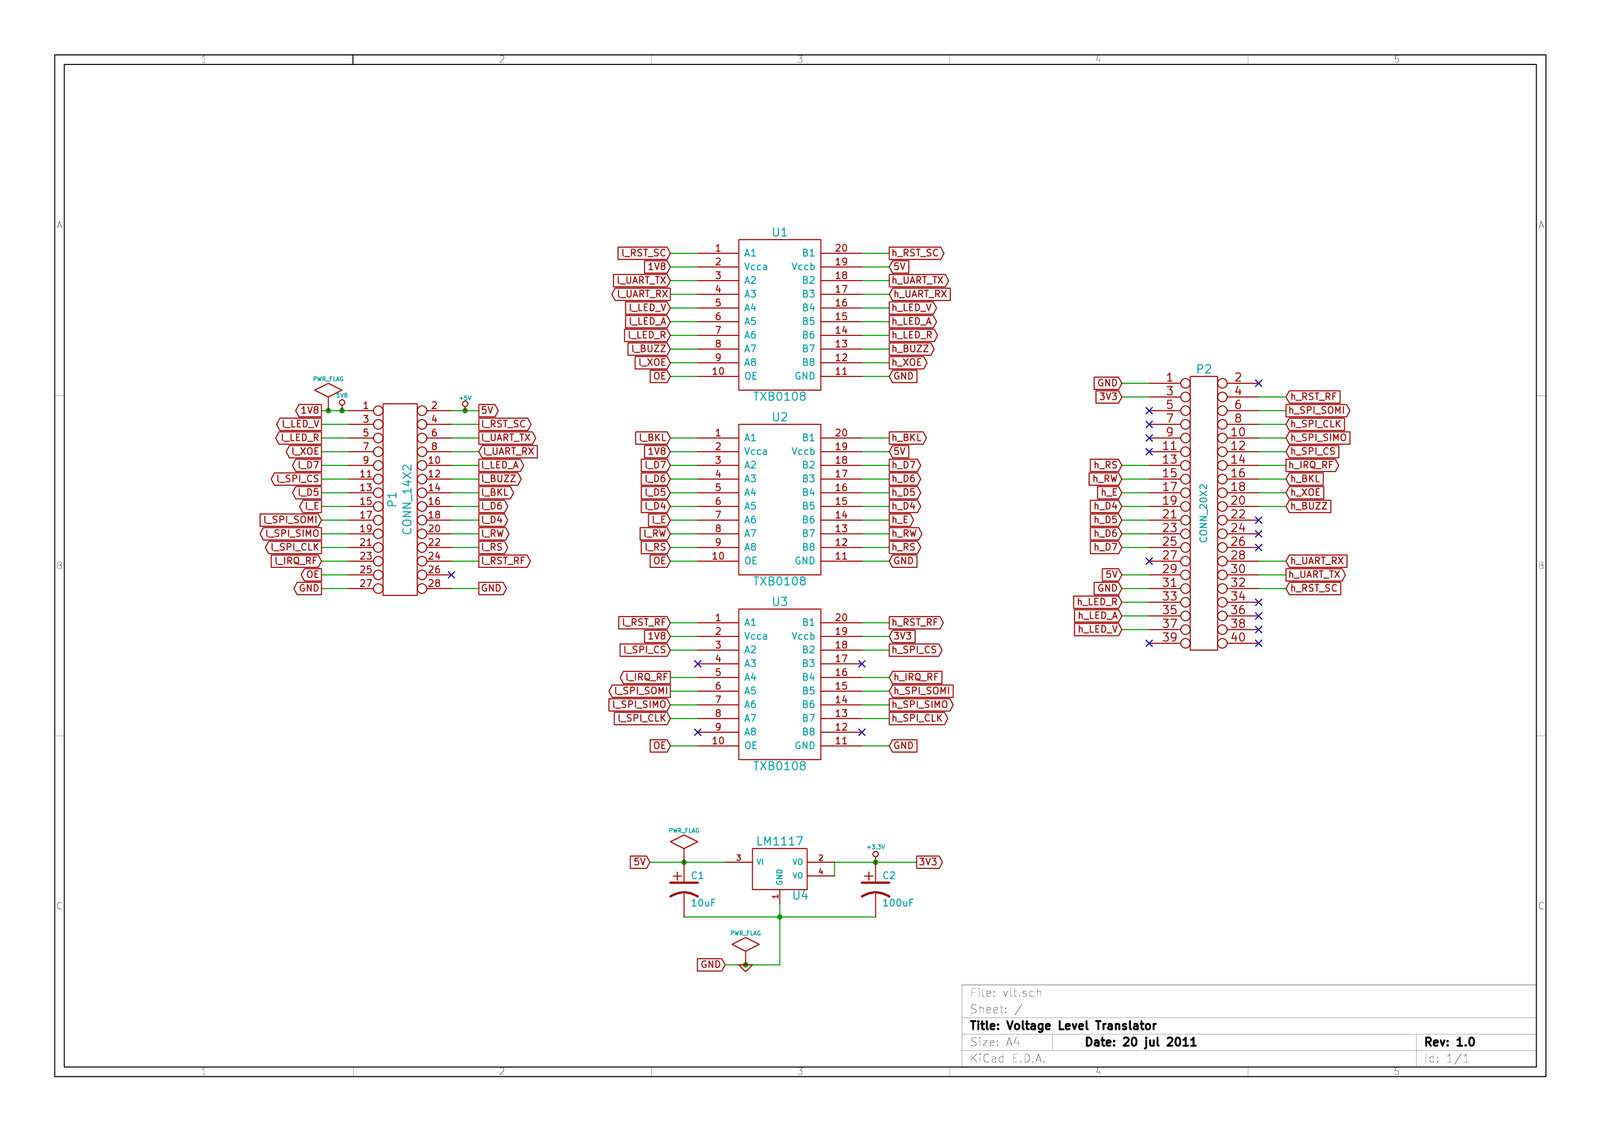
\includegraphics[angle=90]{Imagenes/vlt.jpg}
  \end{center}
  \caption{VLT - Voltage Level Translator}\label{Fig:HW} 
\end{figure}

\subsection{SCUI - Lector de tarjetas de contacto e Interfaz de Usuario}
\begin{longtable}{|l|l|c|c|}
\hline
\multicolumn{1}{|c|}{\textbf{Componente}} & \multicolumn{1}{c|}{\textbf{Descripción}} & \textbf{ Footprint} & \textbf{Valor} \\ \hline
R9 & Resistor 100W 1/4W 1\%  & 3216[1206] & 100W 1/4W  1\% \\ \hline
R10, R13 & Resistor 100KW 1/4W 5\%  & 3216[1206] & 100KW 1/4W   5\% \\ \hline
R11, R12, R14 & Resistor 10KW 1/4W 5\%  & 3216[1206] & 10KW 1/4W   5\% \\ \hline
Q2 & TRANSISTOR, NPN, 300MHZ & SOT23 & MMBT3904 \\ \hline
Q3 & TRANSISTOR, PNP, 250MHZ & SOT23 & MMBT3906 \\ \hline
J2 & SIM socket (6 contacts) & SMD & - \\ \hline
JP3, JP4 & HEADER, 1ROW, 3WAY & T H Pitch 2,54 & 3 pines \\ \hline
X1 & Oscillator 3.579545MHz & SMD & 3.579545 Mhz \\ \hline
ESD1 & Anti ESD & SOT323 & 6V / 150W \\ \hline
\caption{SC}
\label{}
\end{longtable}

%LCD
\begin{longtable}{|l|l|c|c|}
\hline
\multicolumn{1}{|c|}{\textbf{Componente}} & \multicolumn{1}{c|}{\textbf{Descripción}} & \textbf{ Footprint} & \textbf{Valor} \\ \hline
R1 & Resistor 4K7    1/10W     1\% & 1608[0603] & 4,7KW  1/10W   1\% \\ \hline
R2, R8 & Resistor 3R3    1/10W     1\% & 1608[0603] & 3,3W    1/10W   1\% \\ \hline
R3, R4, R5 & Resistor 680R  1/10W     1\% & 1609[0603] & 680W   1/10W   1\% \\ \hline
R6, R7 & Resistor 10K    1/10W     1\% & 1608[0603] & 10KW  1/10W   1\% \\ \hline
RV1 & Preset 15K        1/10W  25\% & SMD & 15KW   1/10W  25\% \\ \hline
Q1 & TRANSISTOR, NPN, 300MHZ & SOT23 & MMBT3904 \\ \hline
S1 & LCD MODULE 16X2 CHARACTER & Pitch 2,54 & - \\ \hline
CONN1 & HEADER FEMALE 16POS.1" TIN & Through Hole & 16 pines \\ \hline
CONN2 & HEADER, 1ROW, 16WAY & T H Pitch 2,54 & 16 pines \\ \hline
LED1 & Led green 5mm & Through Hole & 1,9V,  2mA \\ \hline
LED2 & Led red 5mm & Through Hole & 1,9V,  2mA \\ \hline
LED3 & Led yellow 5mm & Through Hole & 2,4V,  2mA \\ \hline
BUZZ1 & Buzzer & Through Hole & 3~20Vdc, 3~16mA \\ \hline
\caption{LCD}
\label{}
\end{longtable}

\begin{figure}[H]
\centering
  \begin{center}
   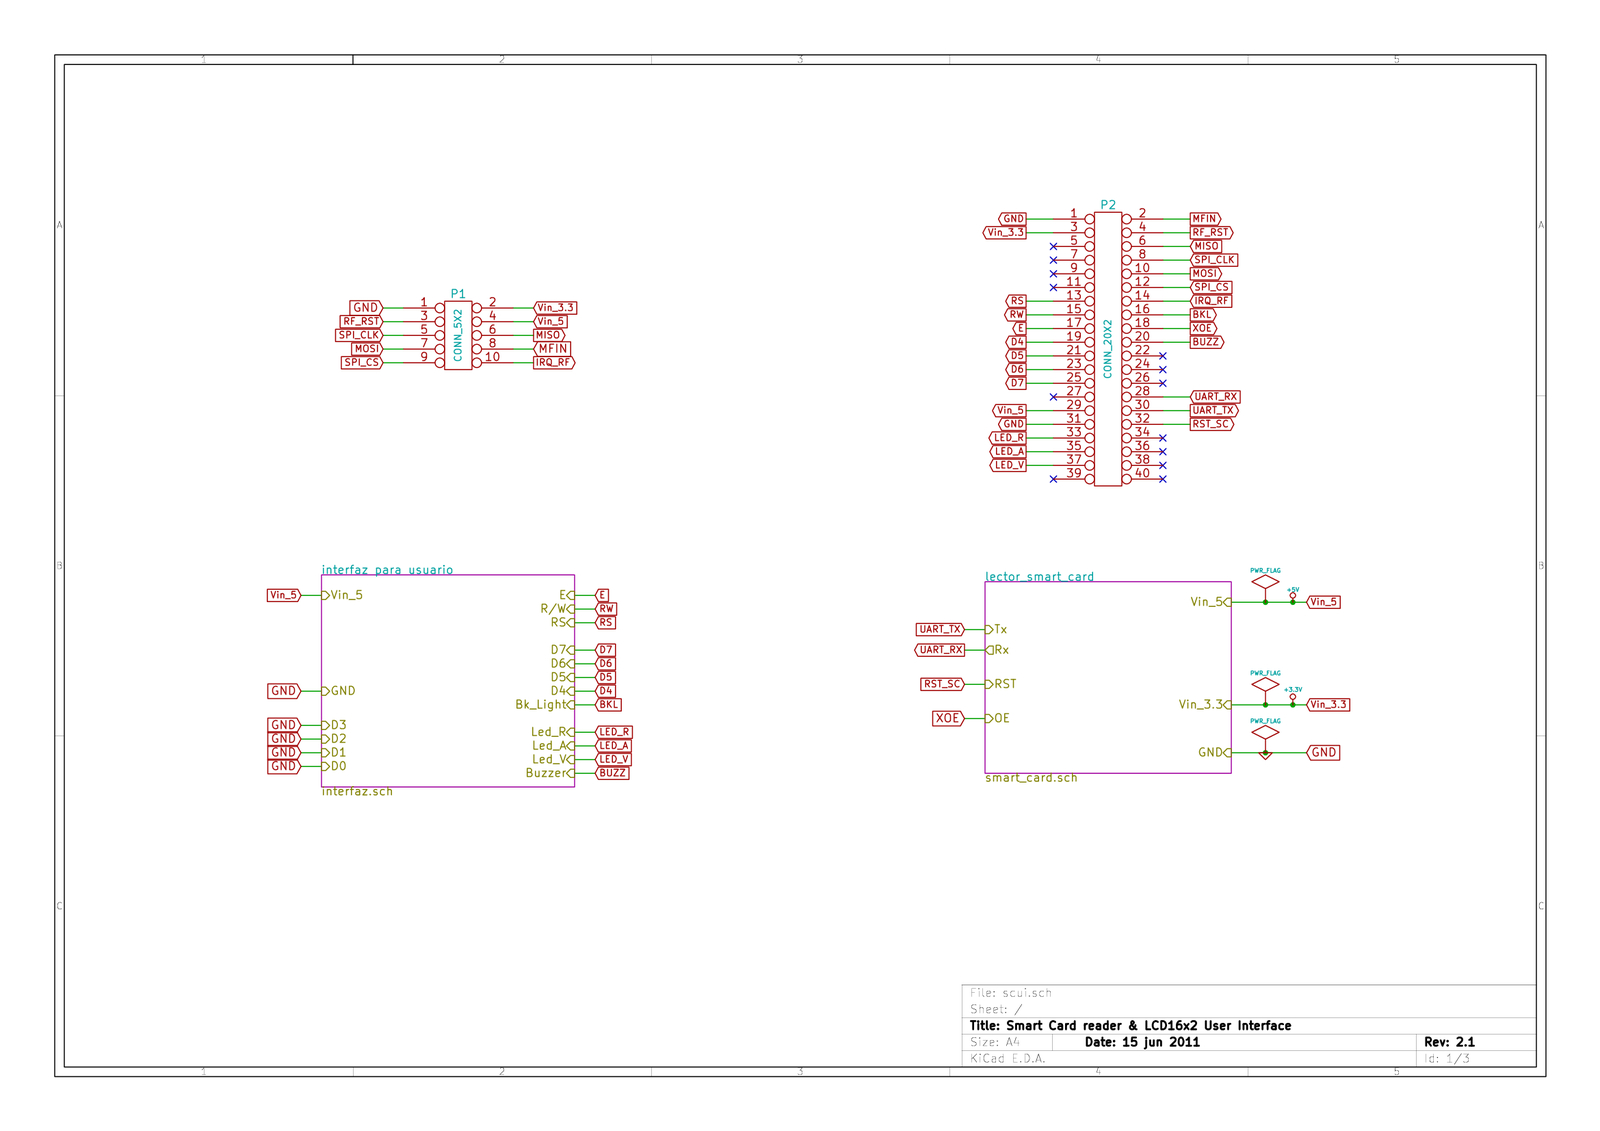
\includegraphics[angle=90]{Imagenes/scui.jpg}
  \end{center}
  \caption{SCUI}\label{Fig:HW} 
\end{figure}

\begin{figure}[H]
\centering
  \begin{center}
   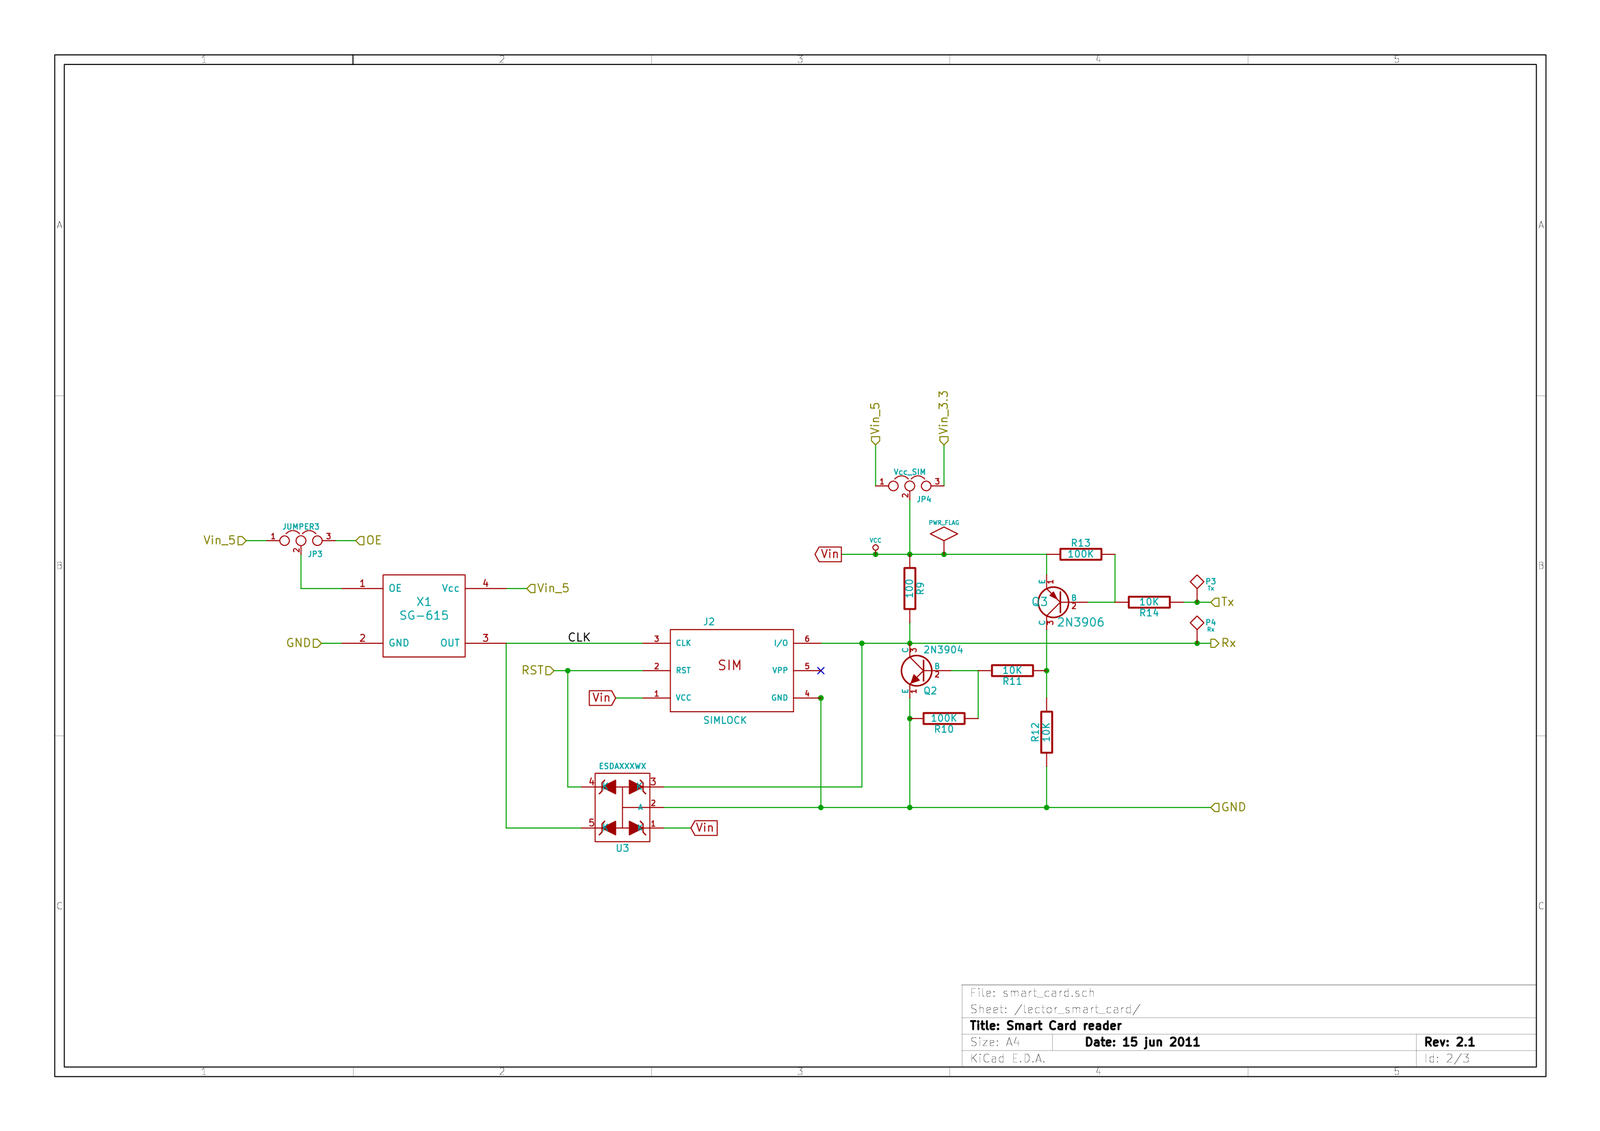
\includegraphics[angle=90]{Imagenes/scui-lector_smart_card.jpg}
  \end{center}
  \caption{VLT - Voltage Level Translator}\label{Fig:HW} 
\end{figure}
%\newpage
\begin{figure}[H]
\centering
  \begin{center}
   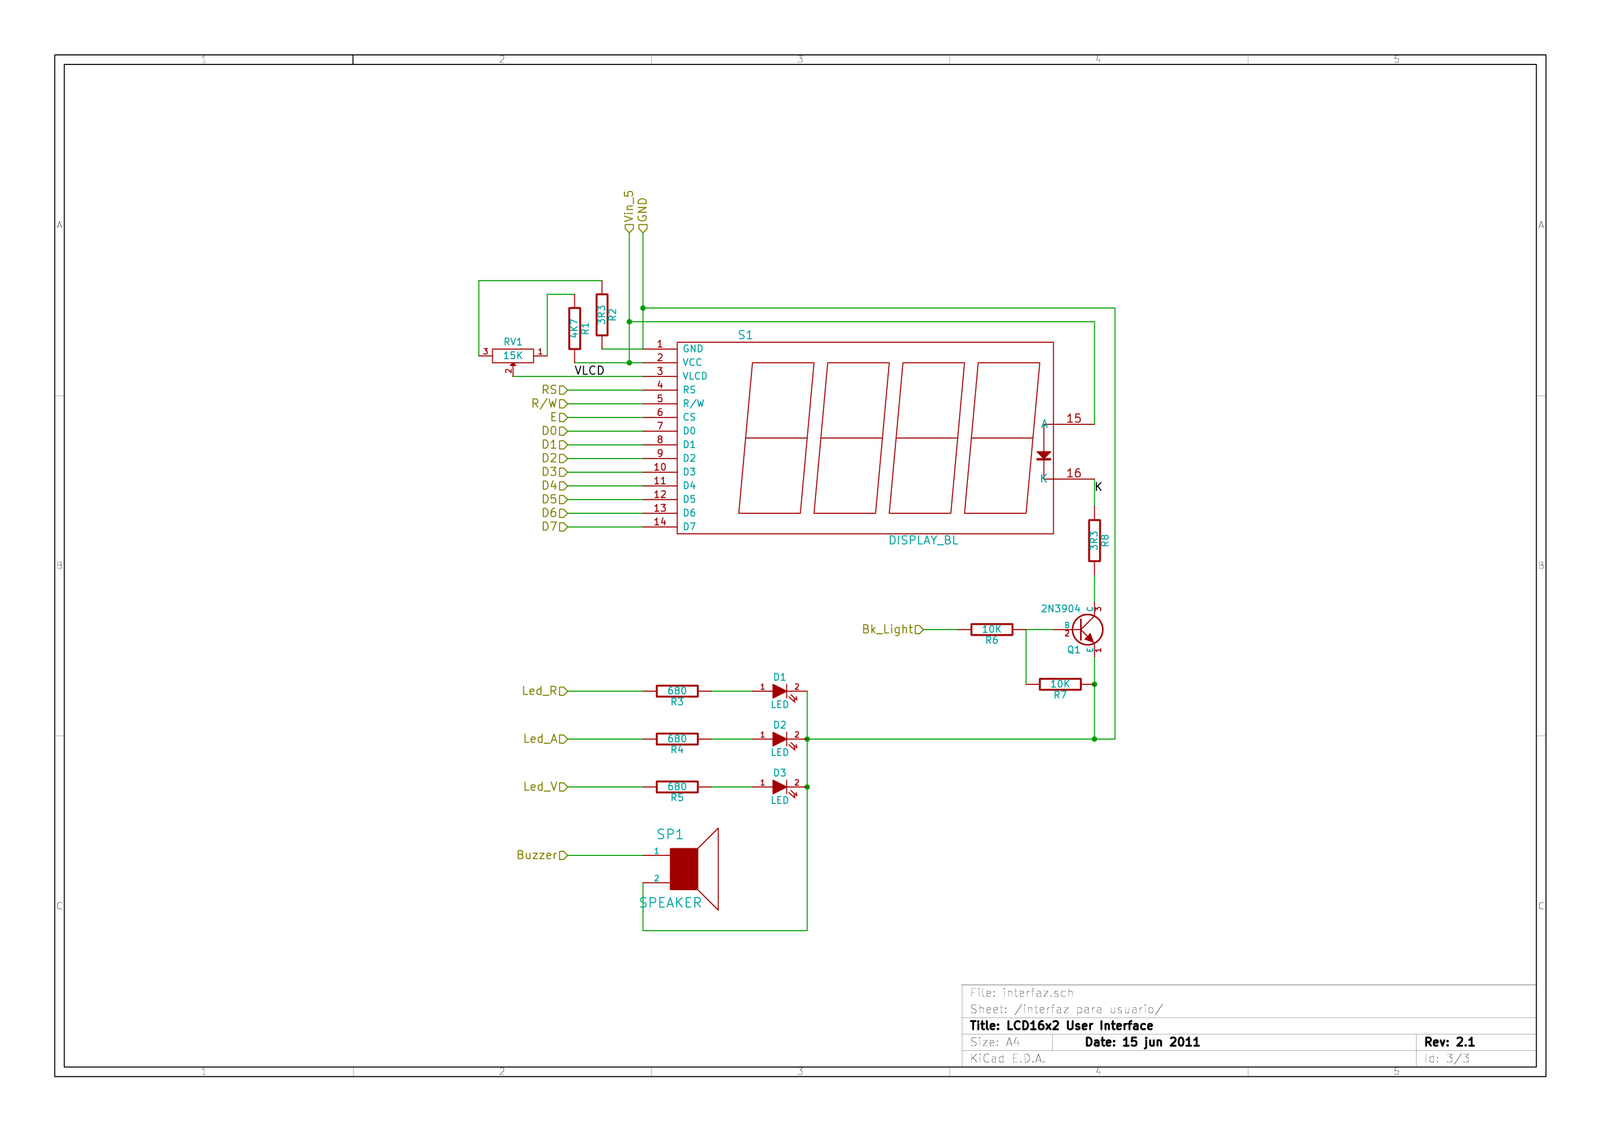
\includegraphics[angle=90]{Imagenes/scui-interfaz_para_usuario.jpg}
  \end{center}
  \caption{VLT - Voltage Level Translator}\label{Fig:HW} 
\end{figure}


\subsection{Lector-Escritor RFID}
\begin{longtable}{|l|l|c|c|}
\hline
\multicolumn{1}{|c|}{\textbf{Componente}} & \multicolumn{1}{c|}{\textbf{Descripción}} & \textbf{ Footprint} & \textbf{Valor} \\ \hline
C1, C2 & Capacitor & 1608[0603] & 10pF,   Ceramic NPO, 2\% \\ \hline
C3, C4 & Capacitor & 1609[0603] & 100pF, Ceramic NPO, 2\% \\ \hline
C5, C6, C7, C8 & Capacitor & 1608[0603] &  NC \\ \hline
R1,  R2 & Resistor & 1608[0603] & 0W,  1/10W,  1\% \\ \hline
\caption{Inductor + Adaptación}
\label{}
\end{longtable}

\begin{longtable}{|l|p{3cm}|c|c|}
\hline
\multicolumn{1}{|c|}{\textbf{Componente}} & \multicolumn{1}{c|}{\textbf{Descripción}} & \textbf{ Footprint} & \textbf{Valor} \\ \hline
C10 & Capacitor & 1610[0603] & 10pF, Ceramic NPO, 2\% \\ \hline
C1, C2 & Capacitor & 1608[0603] & 15pF, Ceramic NPO, 5\% \\ \hline
C12, C13 & Capacitor & 1608[0603] & 56pF, Ceramic NPO, 2\% \\ \hline
C14, C15 & Capacitor & 1608[0603] & 68pF, Ceramic NPO, 1\% \\ \hline
C9 & Capacitor & 1609[0603] & 100pF, Ceramic NPO,  2\% \\ \hline
C16 & Capacitor & 1608[0603] & 1nF, Ceramic NPO, 10\% \\ \hline
C4, C5, C7, C8, C11, C17 & Capacitor & 1608[0603] & 100nF, Ceramic X7R, 10\% \\ \hline
C3, C6, C18 & Capacitor & 1608[0603] & 10uF, Ceramic X5R, 20\% \\ \hline
L1, L2, L3, L6 & Inductor & 2012[0805] & 22nH, 700mA, 5\% \\ \hline
L4, L5 & Inductor & 3225[1210] & 1uH, 400mA, 5\% \\ \hline
R3 & Resistor & 1608[0603] & 50W, 1/10W   1\% \\ \hline
R2 & Resistor & 1608[0603] & 820W, 1/10W   5\% \\ \hline
R1 & Resistor & 1608[0603] & 2,2KW, 1/5W   1\% \\ \hline
U1 & Reader ISO14443 & SO32 & CL RC632 \\ \hline
U2 & Crystal Oscillator, HC49 US SMD & 49USMXL & 13.56MHz, 10pF \\ \hline
U3 & Operational Amplifier (up to 7.5V) & SOT23-5 & OPA354 \\ \hline
CONN1, CONN2 & U.FL-R Connector & U.FL-R-SMT & - \\ \hline
J1 & HEADER, 10WAY, 2ROW & T H Pitch 2,54 & 10 pines \\ \hline
J1b & RECEPTACLE, 10WAY, 2ROW & SMD  Pitch 2,54 & 10 pines \\ \hline
\caption{CL RC632 + filtro EMC}
\label{}
\end{longtable}

\begin{figure}[H]
\centering
  \begin{center}
  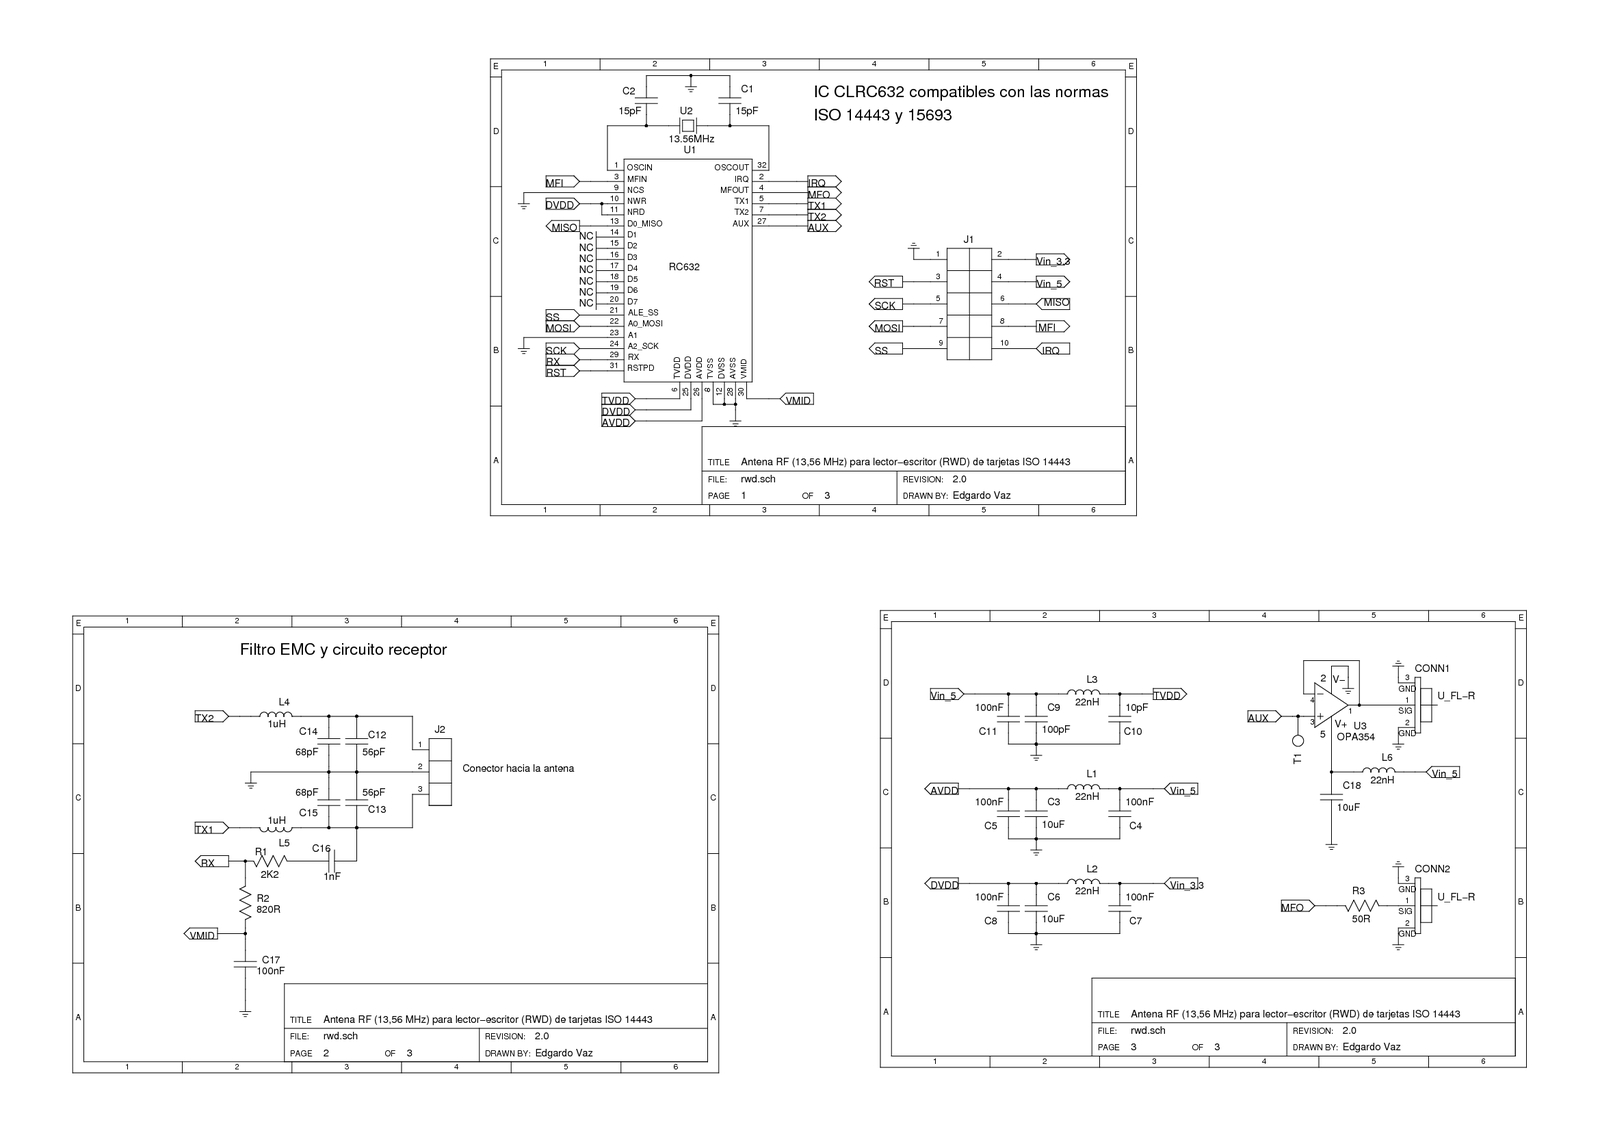
\includegraphics[angle=90]{Imagenes/rfid_rwd.jpg}
  \end{center}
  \caption{rfid coil}\label{Fig:HW} 
\end{figure}

\begin{figure}[H]
\centering
  \begin{center}
  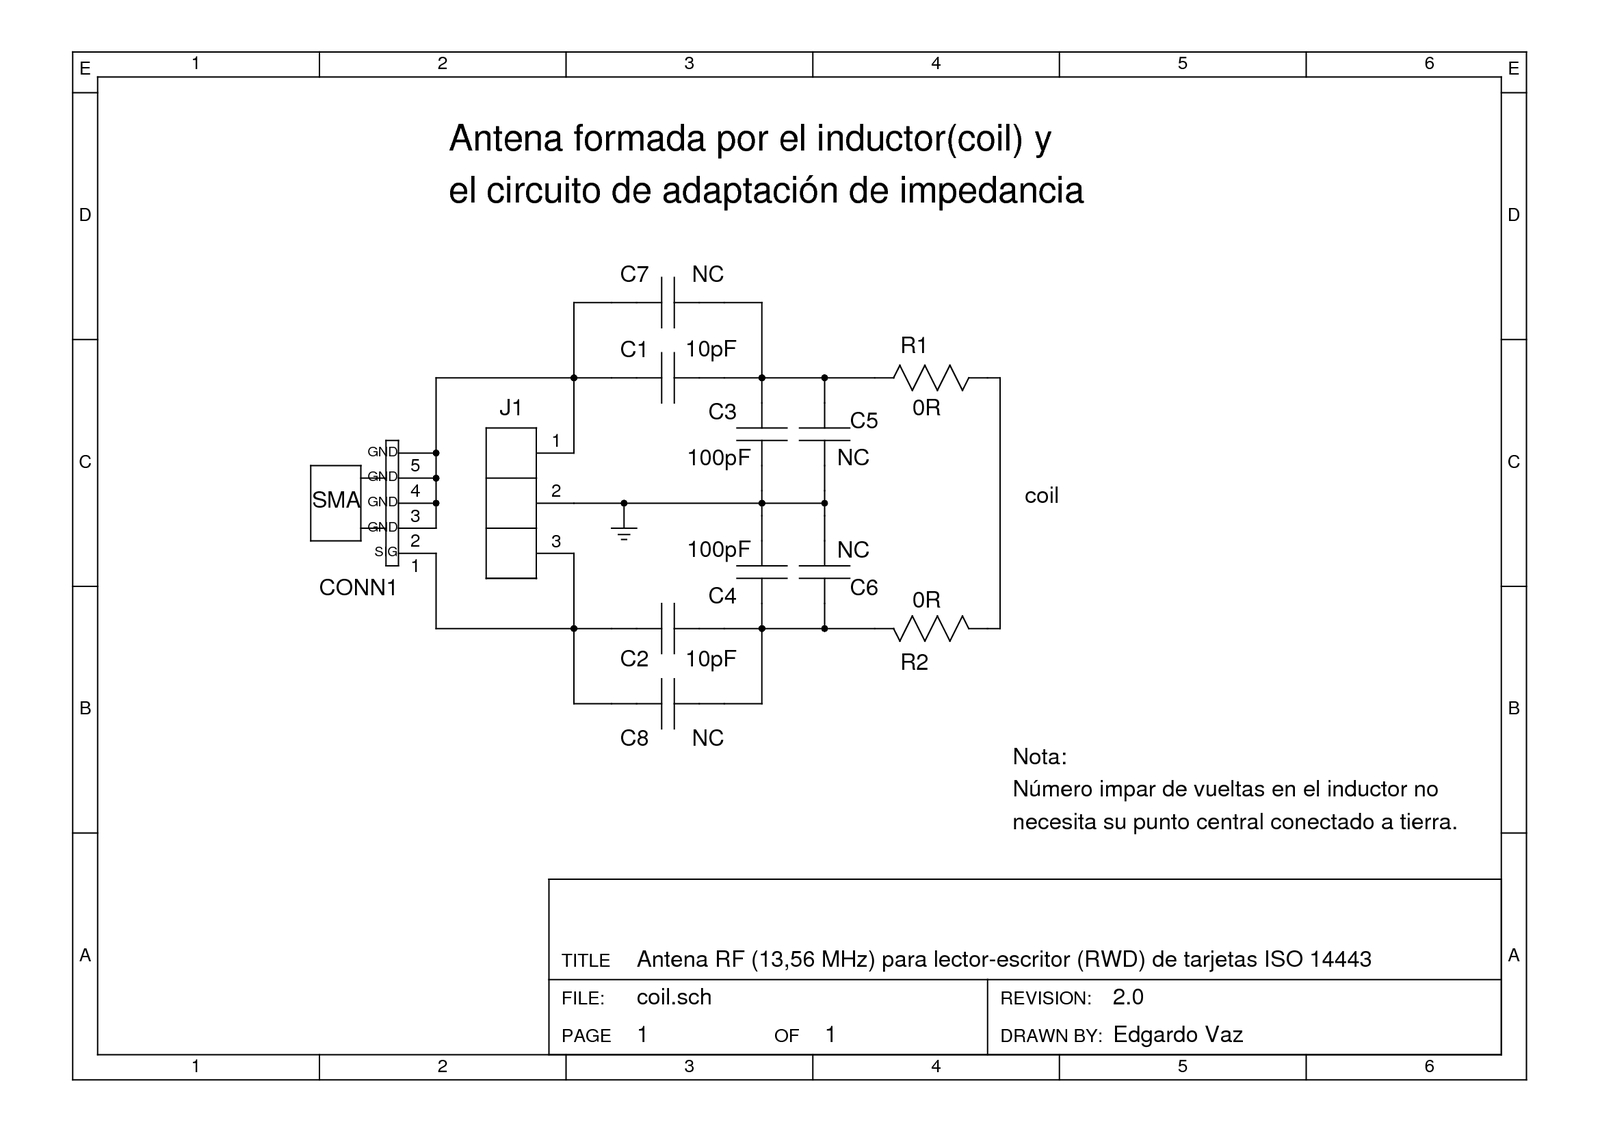
\includegraphics[angle=90]{Imagenes/rfid_coil.jpg}
  \end{center}
  \caption{rfid coil}\label{Fig:HW} 
\end{figure}


\chapter{Software}\label{anx_sw}

\section{Gestor de paquetes opkg}\label{opkg}
Se puede configurar el gestor de paquetes de dos maneras para que encuentre los repositorios desde donde descargar los paquetes para su instalación. 

\bigskip
La primera de ellas es la más prolija y consiste en los siguientes pasos: 

\bigskip
Se crean los archivos xxx-feed.conf (xxx hace referencia a los subdirectorios dentro del repositorio) que contienen la ruta a los repositorios: 

\bigskip
\$ echo src/gz angstrom-feed http://www.angstrom-distribution.org/feeds/unstable/\\
ipk/glibc/armv7a/base  $>$ /etc/opkg/angstrom-feed.conf 

\$ echo src/gz perl-feed http://www.angstrom-distribution.org/feeds/unstable/\\
ipk/glibc/armv7a/perl/ $>$ /etc/opkg/perl-feed.conf 

\$ echo src/gz sdk-feed http://www.angstrom-distribution.org/feeds/unstable/\\
ipk/glibc/sdk/ $>$ /etc/opkg/sdk-feed.conf 

\$ echo src/gz python-feed http://www.angstrom-distribution.org/feeds/unstable/\\
ipk/glibc/armv7a/python/ $>$ /etc/opkg/pyton-feed.conf 

\$ echo src/gz debug-feed http://www.angstrom-distribution.org/feeds/unstable/\\
ipk/glibc/armv7a/debug/ $>$ /etc/opkg/debug-feed.conf 

\$ echo src/gz beagleboard-feed http://www.angstrom-distribution.org/feeds/\\
unstable/ipk/glibc/armv7a/machine/beagleboard/
$>$ /etc/opkg/beagleboard-feed.conf 

\$ echo src/gz noarch-feed http://www.angstrom-distribution.org/feeds/unstable/\\
ipk/glibc/all/ $>$ /etc/opkg/noarch-feed.conf 

\bigskip
Nota: /gz indica que los paquetes están comprimidos con extensión gz. 

\bigskip
Se debe actualizar la lista de paquetes disponibles:

\bigskip
\centerline{\$ opkg update}

\bigskip
El comando anterior crea los archivos /var/lib/opkg/xxx-feed que contienen la lista completa de paquetes en el repositorio. 

\bigskip
Nota: Se puede usar el comando opkg list $|$ wc -l para conocer la lista de paquetes. 

\bigskip
La segunda opción es modificar directamente el archivo /etc/opkg/opkg.conf a continuación de la línea: 

\bigskip
src $<$src-name$>$ $<$source-url$>$

\bigskip
Se agrega lo siguiente: 

\begin{verbatim}
src angstrom-feed http://www.angstrom-distribution.org/
feeds/unstable/ipk/glibc/armv7a/base/ 

src perl-feed http://www.angstrom-distribution.org/feeds/
unstable/ipk/glibc/armv7a/perl/ 

src sdk-feed http://www.angstrom-distribution.org/feeds/
unstable/ipk/glibc/sdk/ 

src python-feed http://www.angstrom-distribution.org/feeds/
unstable/ipk/glibc/armv7a/python/ 

src debug-feed http://www.angstrom-distribution.org/feeds/
unstable/ipk/glibc/armv7a/debug/ 

src beagleboard-feed http://www.angstrom-distribution.org/
feeds/unstable/ipk/glibc/armv7a/machine/beagleboard/ src 
noarch-feed http://www.angstrom-distribution.org/feeds/
unstable/ipk/glibc/all/ 
\end{verbatim}

Luego se actualiza la lista de paquetes:

\centerline{\$ opkg update}

\bigskip
Una vez que se agregan los repositorios es posible instalar paquetes mediante el comando: 

\bigskip
\centerline{\$ opkg install $<$nombre del paquete$>$}

\bigskip
El nombre del paquete puede buscarse en el sitio web que fue pasado como dirección del repositorio en la configuración anterior.

\bigskip
Por más información sobre le uso de este comando, referirse a \cite{AngManual} (ver apéndice \ref{HD}).

\section{Instalación, configuración y uso de SDK}\label{anx_sw_SDK}
Como fue comentado antes, el SDK es generado a partir de la herramienta web Narcissus. Para la instalación se debe tener el archivo (SDK.tar.bz2, por ejemplo) generado.

\bigskip
En el PC de desarrollo se debe hacer lo que sigue:

\bigskip
Se realiza la instalación con el usuario root y luego se explica como proceder con cualquier otro usuario.

\bigskip
\centerline{\$ sudo su}

\bigskip
Se descomprime el SDK en /

\centerline{\$ sudo tar -xf SDK.tar.bz2 -C /}

\bigskip
Se debe haber copiado el directorio angstrom en /usr/local

\bigskip
Luego, se habilita el uso del gestor de paquetes (opkg) y se agraga en el crosscompilador al PATH del sistema. Se debe establecer esta configuración con cada usuario que quiera utilizar la herramienta.

\bigskip
\centerline{\$ . /usr/local/angstrom/arm/environment-setup}

\bigskip
Lo que se tiene es un sistema Angström configurado en el PC de desarrollo con el que se puede actualizar la lista de repositorios, bajar paquetes, compilarlos para la arquitectura deseada, etc.

\bigskip
Actualización de repositorios:

\bigskip
\centerline{\$ opkg-target update}

\bigskip
Instalación de paquetes:

\bigskip
\centerline{\$ opkg-target install $<$paquete$>$}

\bigskip
Actualización de paquetes:

\bigskip
\centerline{\$ opkg-target upgrade}

\bigskip
El uso de opkg-target es solo permitido para el usuario root por un tema de permisos, aunque el uso del crosscompilador es permitido para cualquier usuario siempre y cuando haga lo siguiente cada vez que vaya a utilizar la herramienta:

\bigskip
\centerline{\$ . /usr/local/angstrom/arm/environment-setup}

\bigskip
Para referirse a las herramientas de la arquitectura para la cual se generan los binarios se utiliza el prefijo arm-angstrom-linux-gnueabi-.

\bigskip
Por más detalles referirse a \cite{conf_SDK}.


\section{OpenEmbedded-Bitbake}\label{anx_sw_oe}

Para la instalación, configuración y ejecución de esta herramienta, se deben seguir los pasos en detalle. Se debe tener una buena conexión a internet para la descarga de fuentes, espacio libre en disco duro de no menos de 10GB, buen procesador y paciencia ya que los desarrollos completos demoran varias horas.

\bigskip
Primero se instalan los paquetes previos necesarios. 

\newpage
Paquetes importantes:

\bigskip
\centerline{\$ sudo apt-get install sed wget cvs subversion git-core $\backslash$}

\centerline{coreutils unzip texi2html texinfo docbook-utils $\backslash$}

\centerline{gawk python-pysqlite2 diffstat help2man make gcc build-essential g++ $\backslash$}

\centerline{desktop-file-utils chrpath}

\bigskip
Paquetes secundarios (aceleran los procesos):

\bigskip
\centerline{\$ sudo apt-get install libxml2-utils xmlto python-psyco apr}

\bigskip
Chequear que /bin/sh no tiene un enlace simbólico a “dash”:

\bigskip
\centerline{\$ ls -l /bin/sh}

\bigskip
Debe estar enlazado a “bash”. Si no lo está:

\bigskip
\centerline{\$ sudo dpkg-reconfigure dash}

\bigskip
Aquí seleccionamos NO instalar “dash” como /bin/sh

\bigskip
Compilador para aumentar la velocidad de bitbake:

\bigskip
\centerline{\$ sudo apt-get install python-psyco}

\bigskip
Para versiones de Ubuntu mayores o iguales a la 10.04:

\bigskip
\centerline{\$ sudo su}

\centerline{\$ echo 128 $>$ /proc/sys/vm/mmap\_min\_addr}

\centerline{\$ exit}

\centerline{\$ sudo sysctl -w vm.mmap\_min\_addr=128}


\leftline{Instalación:}

\bigskip
El directorio base seleccionado para el desarrollo con OpenEmbedded es stuff (puede ser otro), y se ubicó en /.

\bigskip
Se crea la estructura de directorios:

\bigskip
\centerline{\$ sudo mkdir -p /stuff/build/conf}

\centerline{\$ cd /stuff/}

\bigskip
Bitbake es la herramienta de construcción que utiliza OpenEmbedded. Está escrita en Python, por lo que no es necesario compilarlo para que funcione.

\bigskip
\centerline{\$ sudo wget http://download.berlios.de/bitbake/bitbake-1.10.2.tar.gz}

\bigskip
Nota: esta es la última versión disponible al momento. Para saber cual es la última versión disponible, entrar a: http://download.berlios.de/bitbake/.

Para las nuevas versiones es necesario tener instalado Python 2.6 o posterior.

\bigskip
Luego se descomprime el tar.gz bajado:

\bigskip
\centerline{\$ sudo tar -xzf bitbake-1.10.2.tar.gz}

\centerline{\$ ls}

\bigskip
Se debe ver un directorio llamado en este caso bitbake-1.10.2 (se puede renombrar a: “bitbake” por comodidad).

\bigskip
Para obtener OpenEmbedded es necesario tener instalado git.

\bigskip
Ahora se hace lo siguiente:

\bigskip
\centerline{\$ cd /stuff}

\centerline{\$ sudo git clone git://git.openembedded.org/openembedded}

\bigskip
Nota: git clone es para hacer un checkout del repositorio. 

Otro repositorio es http://repo.or.cz/r/openembedded.git

\bigskip
Demora mucho. Al finalizar se crea un directorio con el nombre openembedded.

\bigskip
Se recomienda actualizar OpenEmbedded una vez al día:

\bigskip
\centerline{\$ cd /stuff/openembedded}

\centerline{\$ sudo git pull}

\newpage
\leftline{Configuración:}

\bigskip
Se modifica la configuración local, donde se debe indicar todo lo que se quiera crear.

\bigskip
\centerline{\$ cd /stuff/}

\centerline{\$ sudo cp openembedded/conf/local.conf.sample build/conf/local.conf}

\centerline{\$ sudo vi build/conf/local.conf}

\bigskip
Nota: en lugar de vi, se pueden usar nano o incluso gedit. Estos son editores de texto ordenados por complejidad.

\bigskip
En este punto hay que tener cuidado debido a que existen muchas variables a editar y se necesita mucho conocimiento para poder cambiarlas.


La mínima cantidad de variables a editar para un desarrollo correcto son las siguientes:

\bigskip
BBFILES = “/stuff/openembedded/recipes/*/*.bb”

MACHINE = “beagleboard”

DISTRO = “angstrom-2008.1”

PARALLEL\_MAKE = “-j 5”

INHERIT += “rm\_work”

\bigskip
Nota: Los parámetros detallados antes ya existen en el archivo de configuración, algunos deben ser descomentados y/o editados ya que lo único que cambia es el valor asignado.

\bigskip
BBFILES: indica que archivos son considerados durante el desarrollo.

\bigskip
MACHINE: el nombre asociado a la SBC que se esté usando. Para saber el nombre asociado a la SBC se puede ver el contenido del directorio

\leftline{/stuff/openembedded/conf/machine.}

\bigskip
DISTRO: qué versión de la distribución se quiere instalar. Aquí se eligió la última versión estable de Angström, aunque si se pone “angstrom-2010.x”, se obtiene una versión más nueva (no asegura estabilidad). La versión no solo afecta a la distribución sino que la versión del kernel generado va a depender de esta versión. Por ejemplo, con 2008.1 se obtiene un kernel 2.6.32 y con 2010.x se obtiene un kernel 2.6.37. Para saber cuales son las versiones disponibles al momento se puede ver el contenido del directorio 
/stuff/openembedded/conf/distro.

\bigskip
PARALLEL\_MAKE: indica cuantas operaciones simultáneas puede realizar el procesador de la pc de desarrollo. En general el valor se puede calcular como sigue: (cantidad de procesadores)x2 +1. En este caso 5 equivale a una cpu del tipo core2duo.

\bigskip
INHERIT += “rm\_work”: esta opción elimina los fuentes después de haber construido los paquetes. Esto hace que el tamaño del desarrollo en disco, no supere los 10GB. Si esta opción no se elige, se deben tener por lo menos 40GB de espacio libre en disco duro. También se puede decir que si se elige esta opción algunos fuentes deberán ser bajados nuevamente en cada desarrollo, lo que lo puede hacer más lento.


\bigskip
Conviene leer todo el archivo para tener una idea básica de lo que hace. Si en algún lugar se quiere hacer referencia al “home” del usuario, la ruta se debe escribir completa (no se puede $\sim$).

La última línea debe ser borrada (esto es para asegurarse de que se leyó todo). 

\bigskip
\leftline{Ejecución:}

\bigskip
Siempre antes de empezar a desarrollar se debe ejecutar lo siguiente:

\bigskip
\centerline{\$ export BBPATH=/stuff/build:/stuff/openembedded}

\centerline{\$ export PATH=/stuff/bitbake/bin:\$PATH}

\bigskip
Comenzando el desarrollo:

\bigskip
\centerline{\$ cd /stuff/build}

\centerline{\$ bitbake console-image}

\bigskip
Nota: Al ejecutarlo por primera vez, demora varias horas. 

\bigskip
Si aparecen errores como “Please set persistent and cache” o “no se puede acceder al directorio tmp” esto se soluciona dando permisos al directorio stuff:

\bigskip
\centerline{\$ sudo su}

\centerline{\$ chmod -R 777 /stuff}

\bigskip
El comando bitbake console-image baja todos los fuentes y genera todos los binarios necesarios para la ejecución de la  distribución Angström en modo consola. Otra opción, si solo queremos un kernel, es el comando bitbake virtual/kernel, pero para entender bien el funcionamiento del bitbake, la primera vez se recomienda bitbake console-image.

\bigskip
Luego de ejecutado el comando, se crea toda la estructura de directorios.

\bigskip
A continuación se detallan los más importantes:

\bigskip
/stuff/build/tmp/deploy/glibc/images/beagleboard/ 

Aquí se guardan los archivos generados.

\bigskip
/stuff/build/tmp/work/beagleboard-angstrom-linux-gnueabi/

Aquí se encuentran los directorios con los fuentes del kernel y el u-boot.

\section{uImage}\label{anx_sw_uIm}

Se detallan las modificaciones en el archivo board\_omap3beagle.c necesarios para la inicialización correcta de las interfaces SPI y GPIO. Como ya se comentó este archivo está ubicado en /stuff/build/tmp/work/beagleboard-angstrom-linux-gnueabi/linux-omap-.../git/arch/arm/mach-omap2/ y es el encargado de toda la inicialización de las interfaces del sistema.

\bigskip
En el caso de la interfaz SPI se vio que no se lograba un mapeo de la interfaz en /dev, lo que no permitía el acceso a ésta a nivel de usuario. En el caso de la interfaz GPIO se vio que para los pines GPIO no basta con los cambios realizados en el u-boot para establecer su dirección y valor al iniciar el sistema.
A continuación se plantea una posible solución para ambos casos.

\bigskip
\leftline{Cambios asociados al SPI:}

\bigskip
Se creó una estructura (spi\_board\_info beagle\_mcspi\_board\_info) que contempla todas las posibilidades de interfaz SPI en la Beagleboard y agrega información sobre éstas.
En la estrucutra se pueden ver tres formas de representar al SPI: spi3.0, spi3.1 y spi4.0. El microprocesador de la Beagleboard tiene 4 interfaces SPI disponibles de las cuales la 3 y la 4 son accesibles desde el bloque de expansión de la Beagleboard. Además la interfaz spi3 se puede encontrar en dos modalidades 3.0 o 3.1 dependiendo de si se utiliza el CS0 o el CS1 como chip select de la interfaz. La interfaz spi4 solo puede utilizar el CS0.
Es por esto que en la estructura se definen spi3.0, spi3.1 y spi4.0.
Dentro de cada interfaz definida se agrega información sobre la interfaz, como ser el nombre (modalias), la máxima velocidad de transferencia/recepción de datos (max\_speed\_hz), número de bus (bus\_num), chip select (chip\_select) y modo del spi (SPI\_MODE\_1).

\begin{verbatim}
static struct spi_board_info beagle_mcspi_board_info[] = { 
    /* spi 3.0 */ 
    { 
        .modalias	= "spidev", 
        .max_speed_hz	= 48000000, /* 48 Mbps */ 
        .bus_num	= 3, 
        .chip_select	= 0,	 
        .mode = SPI_MODE_1, 
    }, 
    /* spi 3.1 */ 
    { 
        .modalias	= "spidev", 
        .max_speed_hz	= 48000000, /* 48 Mbps */ 
        .bus_num	= 3, 
        .chip_select	= 1,	 
        .mode = SPI_MODE_1, 
    }, 
    /* spi 4.0 */ 
    { 
        .modalias	= "spidev", 
        .max_speed_hz	= 48000000, /* 48 Mbps */ 
        .bus_num	= 4, 
        .chip_select	= 0,	 
        .mode = SPI_MODE_1, 
    }, 
 }; 
\end{verbatim}

\newpage
Luego de definidas las interfaces fue creada una función (omap3\_beagle\_init\_spi\_rf2) que las inicializara.

\begin{verbatim}
static void __init omap3_beagle_init_spi_rf2(void) 
{ 
    printk(KERN_INFO "Usando SPI\n");  
    /* hook the spi ports to the spidev driver */ 
    spi_register_board_info(beagle_mcspi_board_info, 
    ARRAY_SIZE(beagle_mcspi_board_info)); 
}
\end{verbatim}

Para que la función de inicialización de la interfaz SPI pueda ejecutarse, se debe hacer referencia a ésta en la función general de inicialización de interfaces asociada a la Beagleboard (omap3\_beagle\_init).

\begin{verbatim}
omap3_beagle_init_spi_rf2();
\end{verbatim}

Con estos cambios se logró que las interfaces SPI sean accesibles en el espacio de usuario bajo /dev y mapeadas como spidev3.0, spidev3.1, spidev4.0.

\bigskip
\leftline{Cambios asociados al GPIO:}

\bigskip
Se creó una función (gpio\_config\_rf2) que dado un número asociado con el pin GPIO, establece su dirección y valor.

\begin{verbatim}
static void gpio_config_rf2(unsigned gpio, int direction, 
int value) {
  /* Tell the kernel, we want to use the GPIO*/
  if (gpio_request(gpio, "gpio\n") != 0) {
    printk(KERN_ALERT "Unable to request GPIO %d\n", 
    gpio);
  }
  else {
    /* Now tell the kernel that GPIO is an (in-out)put 
    and should be set to value (only as output) */
    switch (direction) {
      case 0: if (gpio_direction_output(gpio, value) != 0) {
                printk(KERN_ALERT "Unable to set GPIO 
                direction for GPIO %d\n", gpio);
              }
              else {
                /* enable direction on userspace */
                if (gpio_export(gpio, 1) != 0){ 
                  printk(KERN_ALERT "Unable to set GPIO 
                  export for GPIO %d\n", gpio);
                }
              }
              break;
      case 1: if (gpio_direction_input(gpio) != 0) {
                printk(KERN_ALERT "Unable to set GPIO 
                direction for GPIO %d\n", gpio);
              }
              else {
                /* enable direction on userspace */
                if (gpio_export(gpio, 1) != 0) { 
                  printk(KERN_ALERT "Unable to set GPIO 
                  export for GPIO %d\n", gpio);
                }
              }
              break;
      default: break;
    }
  }	
}
\end{verbatim}

Se creó la función de inicialización (gpio\_rf2) que establece la configuración de todos los pines GPIO del sistema RF$^{2}$.

\begin{verbatim}
static void __init gpio_rf2(void)
{
    printk(KERN_ALERT "Configurando GPIO RF2...\n");
    gpio_config_rf2(133, 0, 1); /*E*/
    gpio_config_rf2(134, 0, 0); /*D5*/
    gpio_config_rf2(136, 0, 0); /*D7*/
    gpio_config_rf2(137, 0, 0); /*XOE*/
    gpio_config_rf2(138, 0, 0); /*led rojo*/
    gpio_config_rf2(139, 0, 0); /*led_verde*/
    gpio_config_rf2(144, 0, 0); /*RST_SC*/
    gpio_config_rf2(145, 0, 0); /*led_amarillo*/
    gpio_config_rf2(156, 0, 0); /*RW*/
    gpio_config_rf2(157, 0, 0); /*RS*/
    gpio_config_rf2(158, 0, 0); /*Buzzer*/
    gpio_config_rf2(159, 0, 0); /*D4*/
    gpio_config_rf2(161, 0, 0); /*D6*/
    gpio_config_rf2(162, 0, 0); /*Backlight*/
    gpio_config_rf2(168, 0, 1); /*RST_RF*/
    gpio_config_rf2(183, 1, 0); /*IRQ_RF*/
}
\end{verbatim}

Luego, como en el caso de la interfaz SPI, se debe hacer referencia a la función anterior en la función de inicialización del sistema (omap3\_beagle\_init).

\begin{verbatim}
gpio_rf2();
\end{verbatim}

Con estos cambios se logró una cambio en la configuración de los pines GPIO, según la dirección y el valor que les corresponde para el buen funcionamiento del sistema RF$^{2}$.


\section{Instalación y configuración de librfid-tool}\label{ins_conf_librfid}

A continiuación se detalla la instalación y configuración de librfid para su uso con OpenPCD y con el lector/escritor RFID diseñado.

\bigskip
Para comenzar se descarga la biblioteca:

\bigskip
\centerline{\$ svn checkout https://svn.gnumonks.org/trunk/librfid/}

\bigskip
Dentro del directorio raíz, se encuentran una serie de directorios con los fuentes. Los más importantes se detallan a continuación:

\bigskip
utils: en este directorio de encuentran las funciones asociadas con la herramienta librfid-tool. Se destaca librfid-tool.c donde se encuentra la función main de la aplicación librfid-tool.

\bigskip
src: en este directorio se encuentran todos los fuentes de la biblioteca librfid.

\bigskip
include: en este directorio se encuentran todos los encabezados de las funciones de la biblioteca librfid.


\bigskip
\leftline{OpenPCD}

\bigskip
Para comenzar se intentó la comunicación desde el PC para luego pasar a la Beagleboard, ya que existe mucha documentación para el primer caso [REF]. En los dos casos fue necesario compilar la biblioteca para utilizar en la arquitectura elegida.

\bigskip
OpenPCD en PC:

\bigskip
Como primer paso, se conecta el OpenPCD al PC. Para saber si el dispositivo es detectado por la PC, es necesario lo siguiente:

\bigskip
\centerline{\$ lsusb}

\bigskip
Aquí debe aparecer (entre otros dispositivos conectados) un dispositivo con un identificador ID 16c0:076b (vendor:product). 

\bigskip
Nota: En caso de que este dispositivo no aparezca, se debe usar un HUB con alimentación externa.

\bigskip
Compilando librfid:

\bigskip
Para compilar la biblioteca son necesarios los siguientes paquetes: libtool, libusb-dev, libcurl-dev (libcurl4gnutls-dev instalado en este caso).

\bigskip
Se debe ir hasta el directorio donde se encuentra la biblioteca descargada (librfid por ejemplo) y escribir lo siguiente:

\bigskip
\centerline{\$ cd librfid}

\centerline{\$ ./configure}

\centerline{\$ make}

\centerline{\$ sudo make install}


\bigskip
OpenPCD en la Beagleboard:

\bigskip
Antes que nada se debe conectar el OpenPCD a la Beagleboard y verificar que es detectado al igual que en la instalación en el PC:

\bigskip
\centerline{\$ lsusb}

\bigskip
Se tuvo que utilizar un HUB con alimentación externa ya que la Beagleboard no logró ver al OpenPCD.

\bigskip
La compilación se realiza directamente en la Beagleboard.

\bigskip
Al igual que en el caso de la compilación para el uso en un PC, se debieron obtener los paquetes libtool, libusb-dev, libcurl-dev. Para instalar los paquetes se utilizó el siguiente comando:

\bigskip
\centerline{\$ opkg install “paquete”}
 
\bigskip
Se copia la biblioteca (sin compilar) a la Beagleboard y luego:

\bigskip
\centerline{\$ cd librfid}

\centerline{\$ ./configure}

\centerline{\$ make}

\centerline{\$ make install}


\bigskip
Lector-escritor RFID en la Beagleboard:

\bigskip
El lector/escritor RFID se conecta a la Beagleboard a través de una interfaz SPI.
Para habilitar las funcionalidades de la librfid asociadas con la comunicación SPI, es necesario indicar al configurar, que se quiere utilizar esta interfaz a través de la opción $--$enable-spidev. La compilación se realiza en la Beagleboard:

\bigskip
\centerline{\$ cd librfid}

\centerline{\$ ./configure $--$enable-spidev}

\centerline{\$ make}

\centerline{\$ make install}

\bigskip
Con esto se logró compilar la librfid con opciones para utilizar la interfaz SPI

\bigskip
A continuación se explica el uso de librfid-tool:

\bigskip
librfid-tool -[opción]

\bigskip
Dentro de las opciones:

s: realiza una búsqueda de tarjetas RFID hasta encontrar una.

S: loop infinito con la opción “s”, muestra información sobre la tarjeta RFID encontrada en cada paso.

p: especifica el protocolo RFID a utilizar, entre las opciones se encuentran “tcl”, “mifare-classic” y  “mifare-ultralight”.

l: especifica el protocolo de capa 2 a utilizar, entre las opciones se encuentran “ISO14443a”, “ISO14443b” y “ISO15693”.

h: ayuda.

\bigskip
Ejemplos de uso recomendados:

\bigskip
\centerline{\$ librfid-tool -p mifare-classic}

Si encuentra una tarjeta con protocolo Mifare-classic, devuelve la lectura completa de los bloques de memoria de la tarjeta.

\bigskip
\centerline{\$ librfid-tool -S}

Devuelve el UID y el protocolo soportado por la tarjeta.


\section{Depuración de código}\label{depurar}

A continuación se detallan algunos comandos útiles para el depurado de código con GDB:

breakpoint: para colocar un breakpoint. En general se lo llama seguido del nombre de una función de la aplicación.

print: seguido del nombre de una variable, muestra el contenido de la variable durante el proceso de depuración. Si la variable es local a alguna función, el valor de la variable se pierde al salir de la función.

next o “n”: sirve para ir línea a línea en modalidad step-over (sin entrar a las funciones).

step o “s”: sirve para ir línea a línea en modalidad step-into (entrando a las funciones).

backtrace o “bt”: despliega el stack de llamadas a funciones, sirve para saber por donde se pasó y donde se está.

\newpage
\section{Depuración remota}\label{GDB}

A continuación se detalla la configuración de depuración remota con conexión ethernet.

\bigskip
En la Beagleboard:    

\bigskip                							
\centerline{\$ gdbserver localhost: $<$puerto$>$ $<$ejecutable Aplicación$>$ $<$argumentos$>$}

\bigskip
En el pc de desarrollo:

\bigskip
\centerline{\$ gdb}

\centerline{\$ target remote $<$ip\_Beagleboard$>$:$<$puerto$>$}

\bigskip
$<$puerto$>$: número del puerto por el que se conectan. El puerto no debe estar ocupado por otra aplicación. Por ejemplo un número $>$ 2000 funciona correctamente.

\bigskip
$<$ejecutable Aplicación$>$ $<$argumentos$>$: es el nombre de la aplicación que se quiere depurar y si la aplicación necesita algún argumento para ejecutarse correctamente también se deben agregar.

\bigskip
$<$ip\_Beagleboard$>$: es la ip de la Beagleboard.


\section{Preparación de la memoria SD}\label{sd_prep}

Se van a necesitar dos particiones, una FAT32 de más de 32MB y una ext3 (el resto del espacio), la
primer partición (FAT32) debe ser booteable.
Hay dos maneras de hacerlo, una es usando el GParted (modo gráfico) y la otra es por consola.

\subsection{Formateo de la memoria SD}

\leftline{\bf{Formateo utilizando GParted}}

Se instala el GParted:

\centerline{\$ sudo apt-get install gparted}

Se crean las particiones y se les da formato.
Se da click derecho sobre la partición FAT32, gestionar opciones y se marca boot. también se puede dar un nombre a cada partición.


\leftline{\bf{Formateo manual de la memoria SD}}

El siguiente procedimiento se realiza por consola.

\bigskip
Antes que nada se debe saber dónde está la SD (memory card).
Para saberlo se ejecuta en consola: 

\centerline{\$ dmesg}

\bigskip
Se obtiene en parte lo siguiente: 
\begin{verbatim}
sd 3:0:0:0: Attached scsi generic sg1 type 0 
sd 3:0:0:0: [sdb] 7729152 512-byte logical blocks: 
(3.95 GB/3.68 GiB) 
sd 3:0:0:0: [sdb] Write Protect is off 
sd 3:0:0:0: [sdb] Mode Sense: 03 00 00 00 
sd 3:0:0:0: [sdb] Assuming drive cache: write through 
sd 3:0:0:0: [sdb] Assuming drive cache: write through 
sdb: sdb1 
sd 3:0:0:0: [sdb] Assuming drive cache: write through 
sd 3:0:0:0: [sdb] Attached SCSI removable disk 
\end{verbatim}

En este caso la SD está en /dev/sdb 

\bigskip
Se borran las particiones: 

\centerline{\$ sudo fdisk /dev/sdb}

\bigskip
\begin{verbatim}
Command (m for help): o 
Building a new DOS disklabel. Changes will remain in 
memory only, until you decide to write them. After 
that, of course, the previous content won't be 
recoverable. 
Warning: invalid flag 0x0000 of partition table 4 
will be corrected by w(rite) 
\end{verbatim}

Información de la memoria: 

\begin{verbatim}
Command (m for help): p 
Disk /dev/sdb: 3957 MB, 3957325824 bytes 
.... 
\end{verbatim}

Recordar la cantidad de bytes.

\newpage
Se entra en Expert mode: 

\bigskip
\begin{verbatim}
Command (m for help): x 
\end{verbatim}

Se quiere setear la geometría de la siguiente forma: 255 heads, 63 sectors, y se calcula el 
número de cilindros requeridos por la tarjeta: 

\bigskip
C=trunk(B/255/63/512), donde C:cilindros, B:número de bytes de la tarjeta (anotado previamente) 
En este caso: C=trunk(481,117)=481 

\begin{verbatim}
Expert command (m for help): h 
Number of heads (1-256, default 4): 255 
Expert command (m for help): s 
Number of sectors (1-63, default 62): 63 
Warning: setting sector offset for DOS compatiblity 
Expert command (m for help): c 
Number of cylinders (1-1048576, default 1011): 481 
\end{verbatim}


Se va a crear la partición FAT32 y a marcarla como booteable: 

\begin{verbatim}
Expert command (m for help): r 
Command (m for help): n 
Command action 
e extended 
p primary partition (1-4) 
p 
Partition number (1-4): 1 
First cylinder (1-481, default 1): (Enter) 
Using default value 1 
Last cylinder or +size or +sizeM or +sizeK (1-481, 
default 481): +50 
//son como 400MB 
Command (m for help): t 
Selected partition 1 
Hex code (type L to list codes): c 
Changed system type of partition 1 to c (W95 FAT32 
(LBA)) 
Command (m for help): a 
Partition number (1-4): 1 
\end{verbatim}

\newpage
Se crea la segunda partición: 

\begin{verbatim}
Command (m for help): n 
Command action 
e extended 
p primary partition (1-4) 
p 
Partition number (1-4): 2 
First cylinder (52-481, default 52): (Enter) 
Using default value 52 
Last cylinder or +size or +sizeM or +sizeK (52-481, 
default 481):(Enter) 
Using default value 481 
\end{verbatim}

Se imprime para ver como va todo: 

\begin{verbatim}
Command (m for help): p 
Disk /dev/sdb: 3957 MB, 3957325824 bytes 
255 heads, 63 sectors/track, 481 cylinders 
Units = cylinders of 16065 * 512 = 8225280 bytes 
Device Boot 
/dev/sdb1 * 
Start 
1 
End 
Blocks Id System 
51 
409626 c W95 FAT32 (LBA) 
/dev/sdb2 
52 
481 
3453975 83 Linux 
Command (m for help): w 
The partition table has been altered! 
Calling ioctl() to re-read partition table. 
WARNING: Re-reading the partition table failed with 
error 16: Device or resource busy. The kernel still uses 
the old table. The new table will be used at the next reboot. 
WARNING: If you have created or modified any DOS 6.x 
partitions, please see the fdisk manual page for 
additional information. 
Syncing disks. 
\end{verbatim}

\newpage
Se desmontan las particiones creadas: 

\bigskip
\centerline{\$ umount /dev/sdb1}

\centerline{\$ umount /dev/sdb2}

\bigskip
Puede que diga que ya no está montado, en ese caso se sigue igualmente. 

\bigskip
Luego hay que formatear las particiones: 

\bigskip
\centerline{\$ sudo mkfs.msdos -F 32 /dev/sdb1 -n nombre}

\begin{verbatim}
mkfs.msdos 3.0.7 (24 Dec 2009) 
\end{verbatim}

\centerline{\$ sudo mkfs.ext3 /dev/sdb2 -L otroNombre}
\begin{verbatim}
mke2fs 1.41.11 (14-Mar-2010) 
Filesystem label= 
OS type: Linux 
Block size=4096 (log=2) 
Fragment size=4096 (log=2) 
216000 inodes, 863493 blocks 
43174 blocks (5.00%) reserved for the super user 
First data block=0 
Maximum filesystem blocks=402653184 
27 block groups 
32768 blocks per group, 32768 fragments per group 
8000 inodes per group 
Superblock backups stored on blocks: 
32768, 98304, 163840, 229376, 294912, 819200 
Writing inode tables: done 
Creating journal (16384 blocks): done 
Writing superblocks and filesystem accounting information: done
\end{verbatim}

\bigskip
Si dice que no encuentra el dispositivo, se saca la SD y se vuelve a colocar.

\newpage
\subsection{Copia de archivos a la SD}

A partir de aquí se supone que la partición FAT32 tiene el nombre boot y la partición ext3 tiene el nombre rootFS y que los archivos generados se encuentran en el directorio beagleboard ubicado en el home del usuario ($\sim$/beagleboard es su ubicación).

\bigskip
Se realiza por consola. 
Los primeros tres archivos van a la partición FAT32 y el fileSystem (sin descomprimir) va a la 
partición ext3.

\bigskip
\centerline{\$ cd $\sim$/beagleboard}

\centerline{\$ sudo cp MLO /media/boot} 

Nota: El MLO debe ser el primer archivo a copiar.

\bigskip
\centerline{\$ sudo cp u-boot.bin uImage /media/boot}

\centerline{\$ cp fileSystem.tar.gz /media/rootFS}

\bigskip
Se descomprime el fileSystem en la partición ext3.

\bigskip
\centerline{\$ cd /media/rootFS}

\centerline{\$ sudo tar -xvzf fileSystem.tar.gz}

Esto demora un rato.

\centerline{\$ sudo rm -f fileSystem.tar.gz}

Se borra el archivo original.

\bigskip
Se desmonta la memoria SD y queda lista para ser probada. 

\bigskip
\centerline{\$ sync}

\centerline{\$ umount /media/boot}

\centerline{\$ umount /media/rootFS}

\newpage
\section{Configuración en el PC para conexión serial con la Beagleboard}\label{serialBb}

\bigskip
Para la comunicación con la Beagleboard se utilizó el programa minicom el cual se maneja 
desde consola (si se quiere uno con ambiente gráfico, se recomienda cutecom). 
Para configurar minicom se accede a la consola y se escribe lo siguiente: 

\bigskip
\centerline{\$ sudo minicom -s}

\bigskip
Se accede a “Configuración de la puerta serial” y ahí se debe configurar como sigue: 

A - Dispositivo Serial: /dev/ttyUSB0 (si no se encuentra nada, probar con ttyUSB1) 

B - Localización del Archivo de Bloqueo: /var/lock 

C - Programa de Acceso: 

D - Programa de Salida: 

E - Bps/Paridad/Bits: 115200 8N1 

F - Control de Flujo por Hardware: No 

G - Control de Flujo por Software: No 

\bigskip
Luego, para guardar las opciones elegidas se marca la opción “Salvar configuración como dfl”. 

\section{printenv}\label{printenv}

\begin{verbatim}
OMAP3 beagleboard.org # printenv
bootdelay=3 
baudrate=115200 
loadaddr=0x80200000 
rdaddr=0x81600000 
usbtty=cdc_acm 
console=ttyS2,115200n8 
optargs= 
bootscr=boot.scr 
camera=lbcm3m1 
vram=12M 
dvimode=640x480MR-16@60 
defaultdisplay=dvi 
mmcdev=1 
mmcroot=/dev/mmcblk0p2 rw 
mmcrootfstype=ext3 rootwait 
nandroot=/dev/mtdblock4 rw 
nandrootfstype=jffs2 
ramroot=/dev/ram0 rw 
ramrootfstype=ext2 
mmcargs=setenv bootargs console=${console} ${optargs}
mpurate=${mpurate} buddy=${buddy} camera=${camera} 
vram=${vram} omapfb} 
nandargs=setenv bootargs console=${console} ${optargs} 
mpurate=${mpurate} buddy=${buddy} camera=${camera} 
vram=${vram} omapf} 
loadbootscript=fatload mmc ${mmcdev} ${loadaddr} ${bootscr} 
ramargs=setenv bootargs console=${console} ${optargs} 
mpurate=${mpurate} buddy=${buddy} camera=${camera} 
vram=${vram} omapfb} 
loadramdisk=fatload mmc ${mmcdev} ${rdaddr} ramdisk.gz 
bootscript=echo Running bootscript from mmc ...; 
source ${loadaddr} 
loaduimage=fatload mmc ${mmcdev} ${loadaddr} uImage 
mmcboot=echo Booting from mmc ...; run mmcargs; 
bootm ${loadaddr} 
nandboot=echo Booting from nand ...; run nandargs; 
nand read ${loadaddr} 280000 400000; bootm ${loadaddr} 
ramboot=echo Booting from ramdisk ...; run ramargs; 
bootm ${loadaddr} 
dieid#=0968000400000000040365fa1301901a 
mtdids=nand0=nand 
stdin=serial 
stdout=serial 
stderr=serial 
bootcmd=mmc init;fatload mmc 0 80300000 uImage;bootm 80300000 
bootargs=console=ttyS2,115200n8 root=/dev/mmcblk0p2 rw rootwait 
buddy=unknown 
beaglerev=Cx 
mpurate=720
\end{verbatim}

\newpage
\section{Ejemplo de arranque del sistema}\label{arr}

\begin{verbatim}
U-Boot 2009.11-rc1-00601-g3aa4b51 (Jan 05 2010 - 20:56:38) 
OMAP3530-GP ES3.1, CPU-OPP2 L3-165MHz 
OMAP3 Beagle board + LPDDR/NAND 
I2C: ready 
DRAM: 256 MB 
NAND: 256 MiB 
In: serial 
Out: serial 
Err: serial 
Board revision C4 
Die ID #0968000400000000040365fa1301901a 

Hit any key to stop autoboot: 0 
mmc1 is available 
reading uImage 
3194180 bytes read 
## Booting kernel from Legacy Image at 80300000 ... 
Image Name: Angström/2.6.32/beagleboard 
Image Type: ARM Linux Kernel Image (uncompressed) 
Data Size: 3194116 Bytes = 3 MB 
Load Address: 80008000 
Entry Point: 80008000 
Verifying Checksum ... OK 
Loading Kernel Image ... OK 
OK 
Starting kernel ... 
... 
... 
... 

The Angström Distribution beagleboard ttyS2 
Angström 2009.X-test-20100104 beagleboard ttyS2 
beagleboard login: 
\end{verbatim}

Aquí el usuario es root, sin contraseña.


\newpage
\section{Conexión de Beagleboard a internet}\label{BbInternet}

\bigskip
En el PC de desarrollo se debe configurar lo que sigue:

\bigskip
\centerline{\$ sudo gedit /etc/sysctl.conf}

Se debe descomentar la línea que dice net.ipv4.ip\_forward=1 para habilitar el “forwarding” de paquetes.

\bigskip
\centerline{\$ sudo sysctl -p}

\centerline{\$ sudo cat /proc/sys/net/ipv4/ip\_forward}

Lo anterior es para verificar que los cambios fueron hechos de manera correcta.

\bigskip
\centerline{\$ sudo iptables $--$table nat $--$append POSTROUTING $--$out-interface eth0 -j  MASQUERADE}

\centerline{\$ sudo iptables $--$append FORWARD $--$in-interface usb0 -j ACCEPT}

Cuando se refiere a $--$out-interface, se refiere a la interfaz del PC por la que se accede a internet.



\section{Instalación de PCSC-Lite, CCID y pcsc-tools, y agregado de lector serial}\label{anx_pcsc_inst}

A continuación se describe el proceso de instalación en la Beagleboard, el procedimiento para un PC común es el mismo.

\bigskip
Primero se bajan los fuentes asociados a la PCSC-Lite \cite{pcsc/ccid_down}, CCID \cite{pcsc/ccid_down} y pcsc-tools \cite{pcsctools_down}. Luego se envían a la Beagleboard.

\bigskip
Paquetes necesarios en la Beagleboard: libusb-1.0-dev.

\bigskip
\centerline{\$ opkg install libusb-1.0-dev}

\bigskip
PCSC-Lite:

\bigskip
Para la instalación de la PCSC-Lite se usó la biblioteca libusb, aunque se puede hacer con el uso de la biblioteca libudev.
Se supone que los fuentes se encuentran en el directorio pcsclite.

\centerline{\$ cd pcsclite}

\$ ./configure $--$disable-libudev LIBUSB\_CFLAGS=-I/usr/include/libusb-1.0 LIBUSB\_LIBS="-L/usr/lib -lusb-1.0" $--$enable-ipcdir=/var/run/pcscd $--$enable-usbdropdir=/usr/drivers $--$enable-confdir=/etc/reader.conf.d $--$prefix=/usr

\bigskip
LIBUDEV\_CFLAGS: Dirección donde se encuentran los .h asociados con libusb.

LIBUDEV\_LIBS: Dirección donde está libusb.

$--$enable-ipcdir: Dirección donde se guardan archivos relacionados con la comunicación con el demonio de la pcsclite (pcscd).

$--$enable-usbdropdir: Dirección donde se guardan drivers usb (asociado con la instalación del ccid).

$--$enable-confdir: Dirección donde se guardan archivos relacionados con la configuración serial.

$--$prefix:  Dirección a partir de la cual se instalan los archivos necesarios para el correcto funcionamiento de la biblioteca.

\bigskip
\centerline{\$ make}

\centerline{\$ make install}

\bigskip
CCID:

\bigskip
Se supone que los fuentes se encuentran en el directorio ccid.

\bigskip
\centerline{\$ cd ccid}

\$ ./configure LIBUSB\_CFLAGS=-I/usr/include/libusb-1.0 LIBUSB\_LIBS="-L/usr/lib -lusb-1.0" PCSC\_CFLAGS=-I/usr/include/PCSC/ PCSC\_LIBS="-L/usr/lib -lpcsclite" $--$enable-usbdropdir=/usr/drivers $--$prefix=/usr

\centerline{\$ make}

\centerline{\$ make install}

\bigskip
PCSC-TOOLS:

\bigskip
Se supone que los fuentes se encuentran en el directorio pcsc-tools.

\bigskip
\centerline{\$ make}

\centerline{\$ make install}

\bigskip
\bigskip
Pasos para agregar el lector de tarjetas serial, en la biblioteca pcsclite:

\bigskip
Se crea el directorio para drivers de lectores (es posible que ya haya sido creado por CCID al ser instalado). 

\bigskip
\centerline{\$ mkdir /usr/drivers/}

Dentro de este directorio se ubica la biblioteca dinámica del driver para el lector de tarjetas. 

\bigskip	 
\centerline{\$ scp rf2\_sc.so root@172.16.1.14:/usr/drivers}

\bigskip
Luego es necesario crear el archivo de configuración donde se encuentran los parámetros del lector serial. Es posible conocer el directorio donde debe ubicarse el archivo de configuración ejecutando el comando: 

\bigskip
\centerline{\$ pcscd -v}

\bigskip
Se crea el archivo: 

\bigskip
\$ mkdir /etc/reader.conf.d/ 

\$ touch /etc/reader.conf.d/reader.conf 

\bigskip
Se edita el archivo reader.conf agregando las siguientes líneas: 

\begin{verbatim}
##########################################
# Configuration file for pcsc-lite 
# Reader Proyecto-RF2 FING-UDELAR 

FRIENDLYNAME  rf2_sc 
DEVICENAME    /dev/ttyS1 
LIBPATH       /usr/drivers/rf2_sc.so 
CHANNELID     1 
##########################################
\end{verbatim}

CHANNELID indica el número de puerto donde se encuentra el dispositivo: 

\begin{verbatim}
1 ---> /dev/pcsc/1 
2 ---> /dev/pcsc/2 
3 ---> /dev/pcsc/3 
\end{verbatim}

El puerto serial se encuentra realmente en /dev/ttySi, por tanto se debe realizar un enlace simbólico /dev/pcsc/i ---$>$ /dev/ttySi . Para efectuar lo anterior se crea el directorio pcsc bajo dev: 

\bigskip
\centerline{\$ mkdir /dev/pcsc}

\centerline{\$ cd /dev/pcsc}

\centerline{\$ ln -s /dev/ttySi i}

donde i es el número de puerto serial que eusado por el lector de tarjetas. 

\bigskip
Se reinicia el demonio pcscd y se ejecuta la herramienta pcsc\_scan para que muestre el dispositivo: 

\begin{verbatim}
...	
Scanning present readers... 
0: rf2_sc 00 00 

... 
Reader 0: rf2_sc 00 00 
\end{verbatim}


\section{Pruebas sobre las interfaces}

\subsection{led.c}\label{anx_sw_led}

\begin{verbatim}
#include <string.h>
#include <stdio.h>
#include <stdlib.h>
#include <unistd.h>
FILE *fp;

int main(int argc, char** argv)
{
  printf("\n**********************************\n"
  "* Welcome to PIN Blink program *\n"
  "* ....blinking pin 13 on expansion port *\n"
  "* ....rate of 1 Hz............ *\n"
  "**********************************\n");
  //create a variable to store whether we are 
  //sending a '1' or a '0'
  char set_value[4];
  //Integer to keep track of whether we want on or off
  int toggle = 0;
  //Using sysfs we need to write "134" 
  //to /sys/class/gpio/export
  //This will create the folder /sys/class/gpio/gpio134
  if ((fp = fopen("/sys/class/gpio/export", "ab")) == NULL)
  {
    printf("Cannot open export file.\n");
    exit(1);
  }
  //Set pointer to begining of the file
  rewind(fp);
  //Write our value of "134" to the file
  strcpy(set_value,"134");
  fwrite(&set_value, sizeof(char), 3, fp);
  fclose(fp);
  printf("...export file accessed, new pin now accessible\n");
  //SET DIRECTION
  //Open the LED's sysfs file in binary for 
  //reading and writing, store file pointer in fp
  if ((fp = fopen("/sys/class/gpio/gpio134/direction", "rb+")) 
  == NULL)
  {
    printf("Cannot open direction file.\n");
    exit(1);
  }
  //Set pointer to begining of the file
  rewind(fp);
  //Write our value of "out" to the file
  strcpy(set_value,"out");
  fwrite(&set_value, sizeof(char), 3, fp);
  fclose(fp);
  printf("...direction set to output\n");
  //SET VALUE
  //Open the LED's sysfs file in binary for 
  //reading and writing, store file pointer in fp
  if ((fp = fopen("/sys/class/gpio/gpio134/value", "rb+")) 
  == NULL)
  {
    printf("Cannot open value file.\n");
    exit(1);
  }
  //Set pointer to begining of the file
  rewind(fp);
  //Write our value of "1" to the file
  strcpy(set_value,"1");
  fwrite(&set_value, sizeof(char), 1, fp);
  fclose(fp);
  printf("...value set to 1...\n");
  //Run an infinite loop - will require 
  //Ctrl-C to exit this program
  while(1)
  {
    //Set it so we know the starting value 
    //in case something above doesn't leave it as 1
    strcpy(set_value,"1");
    if ((fp = fopen("/sys/class/gpio/gpio134/value", "rb+")) 
    == NULL)
    {
      printf("Cannot open value file.\n");
      exit(1);
    }
    toggle = !toggle;
    if(toggle)
    {
      //Set pointer to begining of the file
      rewind(fp);
      //Write our value of "1" to the file
      strcpy(set_value,"1");
      fwrite(&set_value, sizeof(char), 1, fp);
      fclose(fp);
      printf("...value set to 1...\n");
    }
    else
    {
      //Set pointer to begining of the file
      rewind(fp);
      //Write our value of "0" to the file
      strcpy(set_value,"0");
      fwrite(&set_value, sizeof(char), 1, fp);
      fclose(fp);
      printf("...value set to 0...\n");
    }
    //Pause for one second
    sleep(1);
  }
  return 0;
}
\end{verbatim}



\subsection{uart.c}\label{anx_sw_uart}

\begin{verbatim}
#include <sys/types.h>
#include <sys/stat.h>
#include <fcntl.h>
#include <termios.h>
#include <stdio.h>

#define BAUDRATE B9600
#define SERIALPORT "/dev/ttyS1"
#define _POSIX_SOURCE 1 /* POSIX compliant source */
#define FALSE 0
#define TRUE 1
#define BUFFWRITE 10
#define BUFFREAD 255

int fd; //descriptor del archivo asociado con tty
struct termios oldtio,newtio;

//inicialización
int tty_init (void)
{
  //abrimos el puerto ttyS1
  fd = open(SERIALPORT, O_RDWR | O_NOCTTY ); 
  if(fd<0)
  return 0; //hubo errores
  else
  {
    printf("Puerto %s, abierto. fd: %d\n", SERIALPORT, fd);
    /* save current port settings */
    tcgetattr(fd,&oldtio); 
    //bzero(&newtio, sizeof(newtio));
    newtio.c_cflag = BAUDRATE | CS8 | CLOCAL | CREAD;
    newtio.c_iflag = IGNPAR;
    newtio.c_oflag = 0;
    /* set input mode (non-canonical, no echo,...) */
    newtio.c_lflag = 0;
    /* inter-character timer unused */
    newtio.c_cc[VTIME] = 0;
    /* bloqueo la lectura hasta que llegue 1 caracter */ 
    newtio.c_cc[VMIN] = 1; 
    tcflush(fd, TCIFLUSH);
    tcsetattr(fd,TCSANOW,&newtio);
    return 1; //no hubo errores
  }
}

//envio de un caracter por UART
void escribir (char s[10])
{
  write(fd, s, BUFFWRITE); //escribe el string en UART-Tx
  printf("dato enviado: %s\n", s);
}

//lectura de caracter por UART
char leer (void)
{
  char r[BUFFREAD];
  if(read(fd, r, BUFFREAD) == -1)
  return 0; //No hay datos o se incluyen ceros
  else
  return r[0]; //no hubo errores, se retorna el valor leido
}

int main (void)
{
  //cantidad de caracteres leidos por UART
  int UART_get_return; 
  //indica si se pudo abrir el puerto o no
  int UART_init_return; 
  char buff[BUFFREAD];
  //inicializacion de la UART
  UART_init_return = tty_init(); 
  
  //no se pudo abrir el puerto
  if (UART_init_return == 0) 
  printf("no se pudo abrir el puerto ttyS1.\n");
  else //se pudo abrir el puerto
  {
    char str[10]={'a','s','d','f','g','h','j','k','l','t'};
    escribir(str);
    UART_get_return = read(fd,buff,BUFFREAD);
    
    // 0 = no se encontraron datos en Rx
    if (UART_get_return == 0) 
    printf("no hay datos para leer\n");
    else //1 = dato encontrado
    {
      buff[UART_get_return]=0;
      printf("dato leido: %s:%d\n", buff,UART_get_return);
    }
  }
  tcsetattr(fd,TCSANOW,&oldtio);
}

\end{verbatim}
\part{Compras}
\chapter{Compras}


\section{SBC}
\begin{longtable}{|l|l|c|c|c|}
\hline
\multicolumn{1}{|c|}{\textbf{Componente}} & \multicolumn{1}{c|}{\textbf{Descripción}} & \textbf{Cantidad} & \textbf{Precio x1} & \textbf{Total} \\ \hline
SBC & Beagleboard  RevC4 & 1 & 125 & 125 \\ \hline
Memoria SD & 4GB SDHC Class 6 SD Card & 1 & 15 & 15 \\ \hline
Cable serial DB9 nulo & DB9F Null Modem (RS-232) (6-ft) & 1 & 4 & 4 \\ \hline
Cable conversor usb–serial & USB to DB9M RS-232 (PL-2302) & 1 & 10 & 10 \\ \hline
Cable USB & USB Mini-A to USB A Female, OTG & 1 & 9 & 9 \\ \hline
Cable USB & USB Mini-B Male to USB A Male & 1 & 5 & 5 \\ \hline
Fuente  & 5VDC/2,5A & 1 & 10 & 10 \\ \hline
 &  & \multicolumn{1}{l|}{} & \multicolumn{1}{l|}{} & 178 \\ \hline
\caption{SBC}
\label{}
\end{longtable}

\newpage
\section{PCBs}
\begin{longtable}{|l|l|c|c|c|}
\hline
\multicolumn{1}{|c|}{\textbf{Componente}} & \multicolumn{1}{c|}{\textbf{Descripción}} & \textbf{Cantidad} & \textbf{Precio x1} & \textbf{Total} \\ \hline
VLT & Interfaz entre SBC y SCUI & 1 & 28 & 28 \\ \hline
SCUI & Interfaz de usuario y lector de tarjetas ISO7816 & 1 & 53 & 53 \\ \hline
RWD RFID & Lector/Escritor de tarjetas RFID ISO14443 & 1 & 64 & 64 \\ \hline
 &  & \multicolumn{1}{l|}{} & \multicolumn{1}{l|}{} & 145 \\ \hline
\caption{PCBs}
\label{}
\end{longtable}


\section{VLT}
\begin{longtable}{|l|p{3cm}|p{2cm}|c|c|c|c|}
\hline
\multicolumn{1}{|c|}{\textbf{Componente}} & \multicolumn{1}{c|}{\textbf{Descripción}} & \textbf{ Footprint} & \textbf{Valor} & \textbf{Cantidad} & \textbf{Precio x1} & \textbf{Total} \\ \hline
C1 & Polarized Capacitor (Tantal) & 6032[2312] & 10uF, 25V & 1 & 1,09 & 1,09 \\ \hline
C2 & Polarized Capacitor (Tantal) & 6032[2312] & 100uF, 6V3 & 1 & 1,16 & 1,16 \\ \hline
U4 & Regulador LM1117-3.3 & SOT-223 & 3.3V, 800mA & 1 & 1,1 & 1,1 \\ \hline
U1, U2, U3 & Voltage Level Translator & TSSOP20 & - & 3 & 2,24 & 6,72 \\ \hline
P1 & RECEPTACLE, 28WAY, 2ROW & SMD  Pitch 2,54 & 28 pines & 1 & 4,19 & 4,19 \\ \hline
P2 & RECEPTACLE, 40WAY, 2ROW & SMD  Pitch 2,54 & 40 pines & 1 & 4,36 & 4,36 \\ \hline
P1b & HEADER, 28WAY, 2ROW & T H Pitch 2,54 & 28 pines & 1 & 2 & 2 \\ \hline
P2b & HEADER, 40WAY, 2ROW & T H Pitch 2,54 & 40 pines & 1 & 1,94 & 1,94 \\ \hline
 &  & \multicolumn{1}{l|}{} & \multicolumn{1}{l|}{} & \multicolumn{1}{l|}{} & \multicolumn{1}{l|}{} & 22,56 \\ \hline
\caption{VLT}
\label{}
\end{longtable}


\section{SCUI}
\begin{longtable}{|l|p{2.5cm}|p{2cm}|p{2cm}|c|c|c|}
\hline
\multicolumn{1}{|c|}{\textbf{Componente}} & \multicolumn{1}{c|}{\textbf{Descripción}} & \textbf{ Footprint} & \textbf{Valor} & \textbf{Cantidad} & \textbf{Precio x1} & \textbf{Total} \\ \hline
R9 & Resistor 100W 1/4W 1\%  & 3216[1206] & 100W 1/4W  1\% & 1 & 0,07 & 0,07 \\ \hline
R10, R13 & Resistor 100KW 1/4W 5\%  & 3216[1206] & 100KW 1/4W   5\% & 2 & 0,09 & 0,18 \\ \hline
R11, R12, R14 & Resistor 10KW 1/4W 5\%  & 3216[1206] & 10KW 1/4W   5\% & 3 & 0,08 & 0,24 \\ \hline
Q2 & TRANSISTOR, NPN, 300MHZ & SOT23 & MMBT3904 & 1 & 0,125 & 0,125 \\ \hline
Q3 & TRANSISTOR, PNP, 250MHZ & SOT23 & MMBT3906 & 1 & 0,18 & 0,18 \\ \hline
J2 & SIM socket (6 contacts) & SMD & - & 1 & 1,25 & 1,25 \\ \hline
JP3, JP4 & HEADER, 1ROW, 3WAY & T H Pitch 2,54 & 3 pines & 2 & 0,11 & 0,22 \\ \hline
X1 & Oscillator 3.579545MHz & SMD & 3.579545 Mhz & 1 & 5,25 & 5,25 \\ \hline
ESD1 & Anti ESD & SOT323 & 6V / 150W & 1 & 0,45 & 0,45 \\ \hline
 &  & \multicolumn{1}{l|}{} & \multicolumn{1}{l|}{} & \multicolumn{1}{l|}{} & \multicolumn{1}{l|}{} & 7,965 \\ \hline
\caption{SC}
\label{}
\end{longtable}

%LCD
\begin{longtable}{|l|p{3cm}|p{2cm}|p{2cm}|c|c|c|}
\hline
\multicolumn{1}{|c|}{\textbf{Componente}} & \multicolumn{1}{c|}{\textbf{Descripción}} & \textbf{ Footprint} & \textbf{Valor} & \textbf{Cantidad} & \textbf{Precio x1} & \textbf{Total} \\ \hline
R1 & Resistor 4K7    1/10W     1\% & 1608[0603] & 4,7KW  1/10W   1\% & 1 & 0,05 & 0,05 \\ \hline
R2, R8 & Resistor 3R3    1/10W     1\% & 1608[0603] & 3,3W    1/10W   1\% & 2 & 0,09 & 0,18 \\ \hline
R3, R4, R5 & Resistor 680R  1/10W     1\% & 1609[0603] & 680W   1/10W   1\% & 3 & 0,05 & 0,15 \\ \hline
R6, R7 & Resistor 10K    1/10W     1\% & 1608[0603] & 10KW  1/10W   1\% & 2 & 0,05 & 0,1 \\ \hline
RV1 & Preset 15K        1/10W  25\% & SMD & 15KW   1/10W  25\% & 1 & 0,71 & 0,71 \\ \hline
Q1 & TRANSISTOR, NPN, 300MHZ & SOT23 & MMBT3904 & 1 & 0,125 & 0,125 \\ \hline
S1 & LCD MODULE 16X2 CHARACTER & Pitch 2,54 & - & 1 & 10,85 & 10,85 \\ \hline
CONN1 & HEADER FEMALE 16POS.1" TIN & Through Hole & 16 pines & 1 & 1,25 & 1,25 \\ \hline
CONN2 & HEADER, 1ROW, 16WAY & T H Pitch 2,54 & 16 pines & 1 & 0,155 & 0,155 \\ \hline
LED1 & Led green 5mm & Through Hole & 1,9V,  2mA & 1 & 0,11 & 0,11 \\ \hline
LED2 & Led red 5mm & Through Hole & 1,9V,  2mA & 1 & 0,1 & 0,1 \\ \hline
LED3 & Led yellow 5mm & Through Hole & 2,4V,  2mA & 1 & 0,13 & 0,13 \\ \hline
BUZZ1 & Buzzer & Through Hole & 3~20Vdc, 3~16mA & 1 & 5,31 & 5,31 \\ \hline
 &  & \multicolumn{1}{l|}{} & \multicolumn{1}{l|}{} & \multicolumn{1}{l|}{} & \multicolumn{1}{l|}{} & 19,17 \\ \hline
\caption{LCD}
\label{}
\end{longtable}


\section{Lector/Escritor RFID}
\begin{longtable}{|l|p{2cm}|p{2cm}|p{2.5cm}|c|c|c|}
\hline
\multicolumn{1}{|c|}{\textbf{Componente}} & \multicolumn{1}{c|}{\textbf{Descripción}} & \textbf{ Footprint} & \textbf{Valor} & \textbf{Cantidad} & \textbf{Precio x1} & \textbf{Total} \\ \hline
C1, C2 & Capacitor & 1608[0603] & 10pF,   Ceramic NPO, 2\% & 2 & 0,135 & 0,27 \\ \hline
C3, C4 & Capacitor & 1609[0603] & 100pF, Ceramic NPO, 2\% & 2 & 0,194 & 0,388 \\ \hline
C5, C6, C7, C8 & Capacitor & 1608[0603] &  NC & 4 & - & 0 \\ \hline
R1,  R2 & Resistor & 1608[0603] & 0W,  1/10W,  1\% & 2 & 0,015 & 0,03 \\ \hline
 &  &  &  &  &  & 0,688 \\ \hline
\caption{Inductor + Adaptaci\'on}
\label{}
\end{longtable}



\begin{longtable}{|p{1cm}|p{2.5cm}|p{2cm}|p{2.5cm}|c|c|c|}
\hline
\multicolumn{1}{|c|}{\textbf{Componente}} & \multicolumn{1}{c|}{\textbf{Descripción}} & \textbf{ Footprint} & \textbf{Valor} & \textbf{Cantidad} & \textbf{Precio x1} & \textbf{Total} \\ \hline
C10 & Capacitor & 1610[0603] & 10pF, Ceramic NPO, 2\% & 1 & 0,135 & 0,135 \\ \hline
C1, C2 & Capacitor & 1608[0603] & 15pF, Ceramic NPO, 5\% & 2 & 0,03 & 0,06 \\ \hline
C12, C13 & Capacitor & 1608[0603] & 56pF, Ceramic NPO, 2\% & 2 & 0,194 & 0,388 \\ \hline
C14, C15 & Capacitor & 1608[0603] & 68pF, Ceramic NPO, 1\% & 2 & 0,197 & 0,394 \\ \hline
C9 & Capacitor & 1609[0603] & 100pF, Ceramic NPO,  2\% & 1 & 0,194 & 0,194 \\ \hline
C16 & Capacitor & 1608[0603] & 1nF, Ceramic NPO, 10\% & 1 & 0,08 & 0,08 \\ \hline
C4, C5, C7, C8, C11, C17 & Capacitor & 1608[0603] & 100nF, Ceramic X7R, 10\% & 6 & 0,074 & 0,444 \\ \hline
C3, C6, C18 & Capacitor & 1608[0603] & 10uF, Ceramic X5R, 20\% & 3 & 0,195 & 0,585 \\ \hline
L1, L2, L3, L6 & Inductor & 2012[0805] & 22nH, 700mA, 5\% & 4 & 0,454 & 1,816 \\ \hline
L4, L5 & Inductor & 3225[1210] & 1uH, 400mA, 5\% & 2 & 0,29 & 0,58 \\ \hline
R3 & Resistor & 1608[0603] & 50W, 1/10W   1\% & 1 & 0,268 & 0,268 \\ \hline
R2 & Resistor & 1608[0603] & 820W, 1/10W   5\% & 1 & 0,027 & 0,027 \\ \hline
R1 & Resistor & 1608[0603] & 2,2KW, 1/5W   1\% & 1 & 0,08 & 0,08 \\ \hline
U1 & Reader ISO14443 & SO32 & CL RC632 & 1 & 14,22 & 14,22 \\ \hline
U2 & Crystal Oscillator, HC49 US SMD & 49USMXL & 13.56MHz, 10pF & 1 & 0,98 & 0,98 \\ \hline
U3 & Operational Amplifier (up to 7.5V) & SOT23-5 & OPA354 & 1 & 2,8 & 2,8 \\ \hline
CONN1, CONN2 & U.FL-R Connector & U.FL-R-SMT & - & 2 & 1,76 & 3,52 \\ \hline
J1 & HEADER, 10WAY, 2ROW & T H Pitch 2,54 & 10 pines & 1 & 0,389 & 0,389 \\ \hline
J1b & RECEPTACLE, 10WAY, 2ROW & SMD  Pitch 2,54 & 10 pines & 1 & 2,27 & 2,27 \\ \hline
 &  & \multicolumn{1}{l|}{} & \multicolumn{1}{l|}{} & \multicolumn{1}{l|}{} & \multicolumn{1}{l|}{} & 29,23 \\ \hline
\caption{CL RC632 + filtro EMC}
\label{}
\end{longtable}




% Anexos:
\part{Anexos}
\appendix
%\chapter{Lector/Escritor RFID}\label{anx_antena}

\section{Reglas y Parámetros de Diseño de una Antena RF}

Pasos para el diseño de la antena RF:

\begin{itemize}
\item[A)] Diseñar el inductor, medir su inductancia L y resistencia R (o factor de calidad Q).
\item[B)] Calcular los capacitores para el circuito resonante, que forman junto con el inductor.
\item[C)] Sintonizar el circuito resonante junto con el filtro pasa bajo a la impedancia requerida.
\item[D)] Conectar el circuito resonante a la salida del integrado(TX1 y TX2), verificar la corriente ITVDD y si es necesario sintonizar los componentes para un desempeño óptimo.
\item[E)] Verificar y ajustar el factor de calidad Q.
\item[F)] Verificar y ajustar el circuito receptor.
\end{itemize}

\newpage
\subsection{Diseño del inductor}

Se recomienda usar antenas cuyo inductor tenga forma circular o cuadrado. El valor exacto del inductor es difícil de calcular pero puede ser aproximado por la siguiente ecuación:

\centerline{$ L_{1}[nH]=2 \cdot l_{1} \cdot (ln(\frac{l_{1}}{D_{1}})-K) \cdot N^{1,8}_1$}

\leftline{donde:}
	
\leftline{$l_{1}$ ............... Longitud de una vuelta del conductor (en cm).}

\leftline{$D_{1}$ ............. Diámetro del conductor o ancho del conductor del PCB.}

\leftline{$K$ .............. Factor de forma ($K = 1,07$ antena circular y $K = 1,47$ antena cuadrada).}

\leftline{$N_{1}$ ............. Número de vueltas.}

La antena debe ser simétrica, donde el punto central puede estar conectado a GND. Si esto es así, se sugiere mantener este punto lo más cercano posible al conector de la antena.
El radio de la antena deberá ser $r > 5cm$ para una sola vuelta de cada uno de los inductores simétricos $L_{a}$ y $L_{b}$, o $r < 5cm$ para dos vueltas.
El blindaje de campo eléctrico debe ser conectado a GND.

Los valores de inductancia y resistencia del inductor, si se siguen las reglas de diseño, se encuentran entre: 

$ L = 300nH {...} 2\mu H $

$ R_{coil} =0,5\Omega {...} 5\Omega $


\bigskip
\begin{itshape}
\leftline{Resistor externo}
\end{itshape}


En serie con el inductor se agrega un resistor externo. El valor del mismo se encuentra mediante las ecuaciones:

\centerline{$ Q = \frac{w L}{R_{coil}} \rightarrow R_{coil} = \frac{w L}{Q}$}

\centerline{$ R = 2 \cdot R_{s} + R_{coil} = R_{Sa} + R_{Sb} + R_{coil} $}

donde $R$ es la resistencia total, $R_{Sa}$ y $R_{Sb}$ son cada uno de los resistores externos simétricos.

Definiendo $Q$ entre 20 y 30, se pueden hallar los resistores externos:

$R_{Sa} = R_{Sb} = \frac{1}{2} \cdot (R - R_{coil}) = \frac{wL}{2Q} - \frac{R_{coil}}{2}$ con $w = 2 \pi \cdot 13,56 MHz$


Dejando de lado la influencia de todos los otros componentes en el factor $Q$, este cálculo sólo da una estimación del valor de $R_{S}$, pero esta estimación es necesaria para el cálculo de los capacitores del circuito de resonancia. 

\bigskip
\bigskip
	En muchas aplicaciones prácticas es posible observar que se prescinde del valor de 	resistencia externa $R_{S}$, teniendo en cuenta sólo el valor de resistencia del inductor $R_{coil}$.	

\subsection{Capacitores del circuito resonante}
Gracias a la simertría del circuito es posible simplificar los calculos operando sólo con la mitad del circuito, por tanto los valores del inductor $L$, la resistencia $R$ (incluyendo el resistor externo) y el valor de impedancia requerida de la antena $Z_{ant}$, empleados en los siguientes cálculos son la mitad del valor correspondiente a la totalidad del circuito. 
Aplicando entonces la suma de impedancias a la mitad del cirucito y sabiendo que el resultado tiene que ser real e igual a $Z_{ant}$, es posible hallar los valores del capacitor paralelo $C_{2}$ y el capacitor serie $C_{1}$ mediante las siguientes igualdades:

$C_{2a} = C_{2b} = \frac{L}{\omega^{2}L^{2} + R^{2}} - \frac{R}{( \omega^{2}L^{2} + R^{2}) \omega \sqrt{\frac{Z_{a}}{( \frac{\omega^{2}L^{2} + R^{2}}{R} - Z_{a})}}}$

$C_{1a} = C_{1b} = \frac{1}{\omega \sqrt{Z_{a} \cdot ( \frac{\omega^{2}L^{2} + R^{2}}{R} - Z_{a})}}$

$Z_{ant} = 250 \Omega$


El valor de $Z = 2 \cdot Z_{ant} = 500 \Omega$ podría ser incrementado hasta  $Z = 2 \cdot Z_{ant} = 800 \Omega$ para incrementar la potencia de salida, pero el límite de corriente de salida desde el integrado no debe ser excedido.


\subsection{Sintonizar el circuito resonante}
El circuito todo (incluyendo el filtro pasa bajos) tiene que ser adaptado a una impedancia de aproximadamente 40 $\Omega$ entre TX1 y TX2 (500 $\Omega$ si no tenemos en cuenta el filtro). Donde los valores propuestos para los componentes del filtro son:

\bigskip
\leftline{$L_{0} = 1 \mu H$ (e.g. TDK NL322522T-1R0J)}
\leftline{$C_{01} = 68pF$ (Ceramic NP0, tolerance $\leq \pm 2\%$)}
\leftline{$C_{02} = 56pF$ (Ceramic NP0, tolerance $\leq \pm 2\%$)}

\newpage
Con estos valores, la frecuencia de resonancia del filtro se encuentra centrada en $14,4 MHz (13,56 MHz + 847,5 KHz)$. Esto mejora la performance en dos formas:


\begin{itemize}
\item[a)] Incrementa la relación señal a ruido de la señal recibida.
\item[b)] Decrementa el sobretiro de los pulsos transmitidos, mejorando la calidad de la señal transmitida.
\end{itemize}

El procedimiento para sintonizar el circuito, es el siguiente:

Los materiales necesarios son:
\begin{itemize}
\item[-] Generador de señales ($13,56 MHz$).
\item[-] Osciloscopio con puntas de prueba.
\item[-] Resistor de referencia ($40 \Omega$).
\end{itemize}

\bigskip
Se debe conectar las puntas del osciloscopio a la salida del generador y en paralelo un resistor de referencia de $40 \Omega$ ($500 \Omega$ en caso de sintonizar el circuito sin conectar el filtro pasa bajos).

\bigskip
\begin{itshape}
\leftline{Calibración}
\end{itshape}

Se genera una señal sinusoidal de frecuencia $13,56 MHz$ y de amplitud entre $2V$ y $5V$.
El osciloscopio se configura para observar las figuras de Lissajous, con la escala del eje X dos veces la del eje Y.
Se calibra el capacitor, $C_{cal}$, de la punta de prueba del osciloscopio hasta que la figura de Lissajous sea un segmento de recta, inclinado $45º$.

\bigskip
\begin{itshape}
\leftline{Sintonizado}
\end{itshape}

Luego de la calibración se sustituye el resistor de referencia por la antena y se sintoniza la misma variando los capacitores $C_{1}$ y $C_{2}$, hasta que se obtenga una figura como la obtenida en el caso anterior. En ese momento la antena se encuentra sintonizada.


En caso de contar con un analizador de redes, el método anterior puede ser evitado, ya que es posible sintonizar el circuito buscando que la impedancia en el diagrama de Smith se ubique sobre el eje real al alcanzar la frecuencia de trabajo, en este caso $13,56 MHz$.


\subsection{Valor de ITVDD}

El integrado de la familia Micore, entrega a la salida una señal cuadrada, con valor de pico a pico $U_{TxAC} = 2,5V_{pp}$ centrada en el valor de continua  $U_{TxDC} = 2,5V$, con una frecuencia $f_{0} = 13,56 MHz$ y un máximo de salida de corriente: 


\centerline{$I_{TVDD} \leq 150mA$}


Esto significa que la salida TX oscila entre $0V$ y $5V$. TX1 y TX2 usualmente están desfasados $180º$, dependiendo de la configuración del bit 3 (TX2Inv) del registro Tx-Control (ver hoja de datos del integrado RC632).


\subsection{Factor de calidad Q}

El factor de calidad $Q$ está directamente asociado con la forma de los pulsos modulados, ésto puede ser usado para verificar el valor del factor.

\bigskip
Un osciloscopio con al menos $50 MHz$ de ancho de banda puede ser usado para observar la forma de los pulsos; donde los canales son conectados de la siguiente forma:

\bigskip
CH1:   La punta de prueba conectada en este canal forma un loop con su línea de tierra para generar el acoplamiento necesario al estar próxima a la antena.

\bigskip
CH2:   Este canal es conectado a la salida del pin 4 (MFout) de integrado y es usado como canal de disparo.
\bigskip

El registro MFoutSelect (26h) es configurado con los valores:
\begin{itemize}	
\item[]	“2” para que la señal sea modulada con código Miller.
\item[]	“3” para flujo de datos serial (sin código Miller).
\item[]	Ver hoja de datos del integrado RC632 por más detalles.	
\end{itemize}	

Es recomendado verificar que la forma de los pulsos cumpla con lo establecido en la norma ISO14443. La figura \ref{Fig:pulso14443} muestra como son estos pulsos.


Para garantizar que la antena se encuentre bien sintonizada y el factor $Q$ sea el correcto, debe verificarse que:


\begin{itemize}
\item[i.] La señal caiga debajo del $5\%$ de su valor máximo (sin tener en cuenta el sobretiro).
\item[ii.] El tiempo $t2$ debe estar limitado entre:  $0,7\mu s < t2 < 1,4\mu s$.
\end{itemize}

Si $t2 < 0,7\mu s$, el factor $Q$ es muy alto (mayor que 35), por lo tanto la resistencia externa $R_{ext}$ debe ser incrementada.

\bigskip
Si  $t2 > 1,4\mu s$ el factor $Q$ es muy bajo, la distancia de operación no será cumplida y por lo tanto $R_{ext}$ debe ser decrementada.

\bigskip
La tabla siguiente muestra la duración de los pulsos en $\mu s$ de acuerdo a la norma ISO 14443.

\begin{longtable}{|l|c|c|c|c|r|}
\hline
\multicolumn{1}{|c|}{\textbf{Pulses length}} & \textbf{t1} & \textbf{t2 min} & \textbf{t3 max} & \textbf{t4 max} \\ \hline

%Pulses length 				t1          t2 min	          t3 max          t4 max 
T1 MAX 			 &          3.0    &       0.7    &            1.0 &                0.4 \\ \hline
T1 MIN 			 &          2.0    &       0.7    &            1.0 &                0.4 \\ \hline
\caption{Duración de los pulsos en $\mu s$ - ISO 14443}
\label{}
\end{longtable}

\begin{figure}[H]
\centering
  \begin{center}
  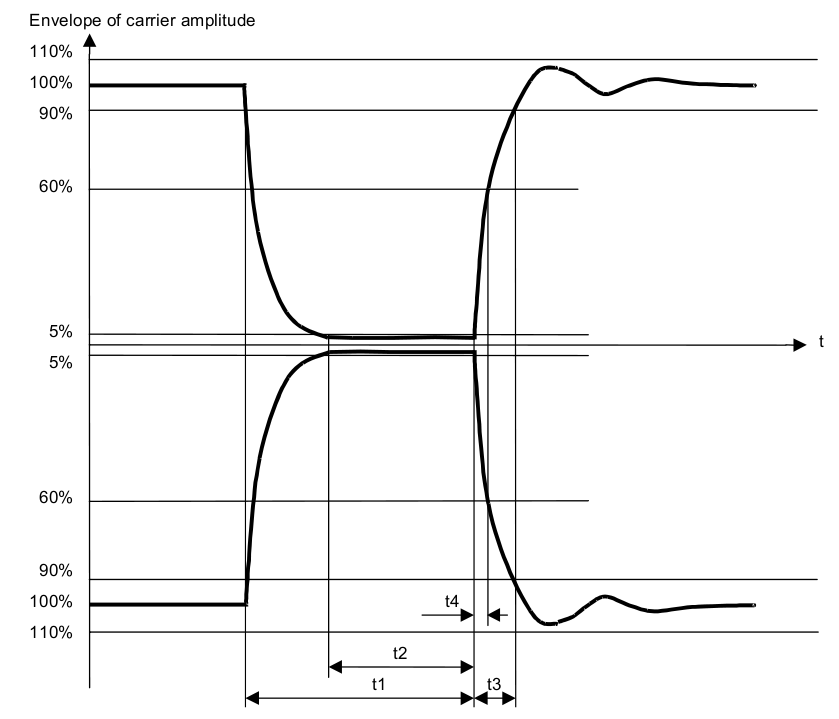
\includegraphics[scale=.4]{Imagenes/anexo1.png} 
  \end{center}
  \caption{Forma de pulso acorde a la norma ISO 14443}\label{Fig:pulso14443} 
\end{figure}


\subsection{Circuito receptor}

Cuando ya se han tomado en cuenta todos los cuidados en el diseño del transmisor, el circuito receptor debe ser conectado y ajustado.
Los valores de los componentes sugeridos en el circuito receptor son los siguientes:

\bigskip
	$C_{3} = 1nF$ 			(Ceramic NP0, tolerance $\leq \pm 10\%$) 
	
	$C_{4} = 100nF$ 			(Ceramic X7R, tolerance $\leq \pm 10\%$) 
	
	$R_{1} = 470 \Omega {...} 4.7 k \Omega $ 
	
	$R_{2} = 820 \Omega $
	
\bigskip
Dos reglas deben ser tenidas en cuenta para este circuito:

\begin{itemize}
\item[i.] El nivel de tensión de continua, DC, en la entrada Rx tiene que ser mantenido a $V_{mid}$ (por eso es necesario $R_{2}$ y $C_{4}$, ver figura \ref{Fig:RFID4}).
\item[ii.] El nivel de tensión de alterna, AC, en la entrada Rx debe ser mantenido entre los siguientes límites: $1,5V_{pp} < V_{Rx} < 3,0V_{pp}$.
\end{itemize}	

\bigskip
Si $V_{Rx} > 3,0V_{pp}$,  $R_{1}$ debe ser incrementada.

\bigskip
Si $V_{Rx} < 1,5V_{pp}$,  $R_{1}$ debe ser decrementada.

\bigskip
El voltaje a la entrada Rx debe ser verificado con y sin presencia de una tarjeta entre los límites máximo y mínimo de distancia de operación.

\bigskip
\begin{itshape}
El valor límite  $V_{Rx}= 3,0V_{pp}$ no debe ser excedido, un valor mayor puede causar fallos en la recepción.
\end{itshape}

\bigskip
\bigskip
\leftline{\bf{Otros puntos a tener en cuenta}}

\bigskip
\leftline{PCB}

\bigskip
La parte más crítica de todo el circuito analógico es el directamente conectado al integrado, o sea el filtro pasa bajos y la conexión de TVDD a la fuente de alimentación.
Entonces, por un lado un filtro puede ser usado para la conexión a la fuente de alimentación.
Por otro lado el diseño del filtro a la salida del integrado, formado por $L_{0}$ y $C_{0}$, debe ser considerado con mucho cuidado. \begin{itshape} El área y la distancia del filtro al integrado deben ser mantenidas lo más pequeñas posibles. Es recomendado además un plano de tierra.	
\end{itshape}

\bigskip
La figura \ref{Fig:RFID4} muestra un esquemático del diseño de una antena:

\begin{figure}[H]
\centering
  \begin{center}
  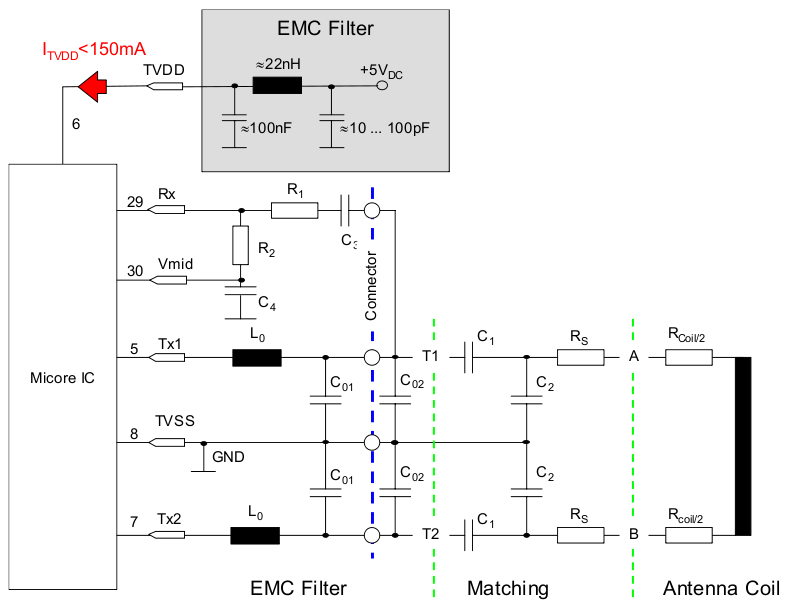
\includegraphics[scale=.4]{Imagenes/anexo2.png} 
  \end{center}
  \caption{Esquema de una antena, identificando sus principales secciones}\label{Fig:RFID4} 
\end{figure}


\bigskip
\leftline{Filtro de entrada de alimentación}

\bigskip
Aunque no sería necesario, un filtro puede ser conectado a la entrada TVDD para mejorar los siguientes puntos:

\begin{itemize}
\item[a)] suprimir ruido llegado desde la fuente de alimentación.
\item[b)] suprimir armónicos provenientes desde el transmisor.
\end{itemize}

Filtros idénticos pueden ser ubicados en las entradas AVDD y DVDD.

\newpage
\leftline{Blindaje}

\bigskip
El blindaje eléctrico absorbe el campo eléctrico generado por la antena. Para construir un blindaje, es recomendable usar un PCB de al menos 4 capas, donde el loop del blindaje se encuentra en las 2 capas externas. Este loop no debe ser cerrado y debe estar conectado en su punto central al sistema de tierra mediante una vía. Los extremos de la bobina deben ser ruteados próximos entre sí para evitar inductancias adicionales.  La figura \ref{Fig:blindaje} da una idea de como debe ser un blindaje: 


\begin{figure}[H]
\centering
  \begin{center}
  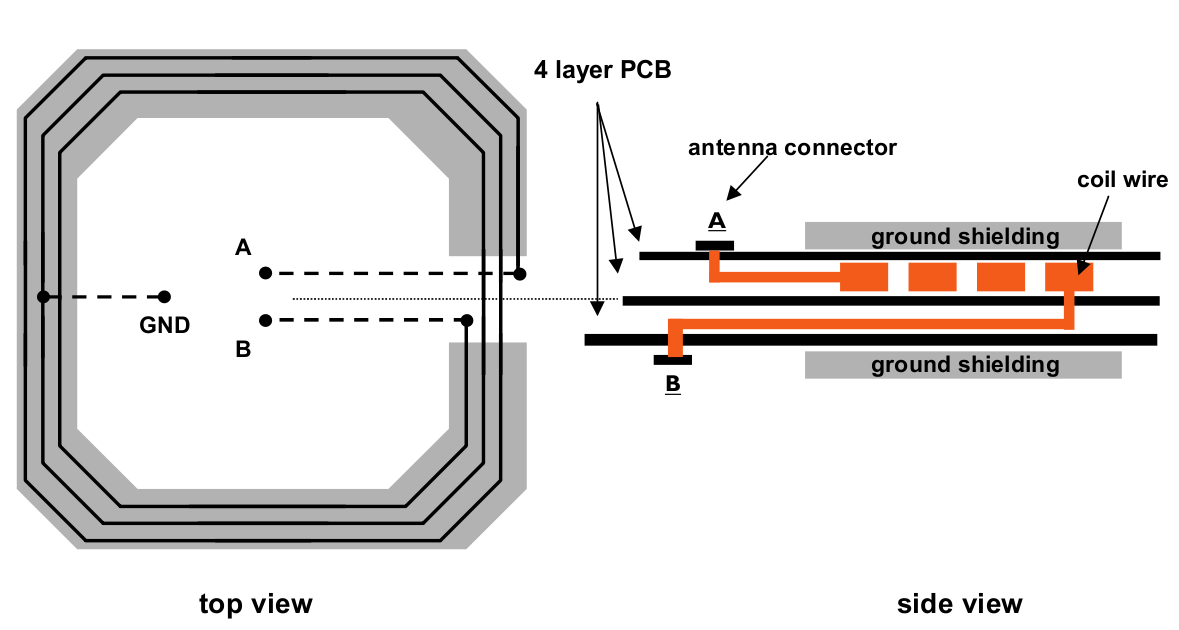
\includegraphics[scale=.3]{Imagenes/anexo3.png} 
  \end{center}
  \caption{Blindaje de una antena en un diseño de 4 capas}\label{Fig:blindaje} 
\end{figure}



% Bibliografía:
\part{Bibliografía}
%\bibliographystyle{ieeetr}
%\bibliography{Bibliografia/biblio}

\end{document}
